% ******************************* PhD Thesis Template **************************
% Please have a look at the README.md file for info on how to use the template

% \documentclass[a4paper,12pt,times,numbered,print,index]{PhDThesisPSnPDF}
\documentclass[chapter,a4paper,12pt,times]{PhDThesisPSnPDF}

% ******************************************************************************
% ******************************* Class Options ********************************
% *********************** See README for more details **************************
% ******************************************************************************

% `a4paper'(The University of Cambridge PhD thesis guidelines recommends a page
% size a4 - default option) or `a5paper': A5 Paper size is also allowed as per
% the Cambridge University Engineering Deparment guidelines for PhD thesis
%
% `11pt' or `12pt'(default): Font Size 10pt is NOT recommended by the University
% guidelines
%
% `oneside' or `twoside'(default): Printing double side (twoside) or single
% side.
%
% `print': Use `print' for print version with appropriate margins and page
% layout. Leaving the options field blank will activate Online version.
%
% `index': For index at the end of the thesis
%
% `draftclassic': For draft mode without loading any images (same as draft in book)
%
% `draft': Special draft mode with line numbers, images, and water mark with
% timestamp and custom text. Position of the text can also be modified.
%
% `abstract': To generate only the title page and abstract page with
% dissertation title and name, to submit to the Student Registry
%
% `chapter`: This option enables only the specified chapter and it's references
%  Useful for review and corrections.
%
% ************************* Custom Page Margins ********************************
%
% `custommargin`: Use `custommargin' in options to activate custom page margins,
% which can be defined in the preamble.tex. Custom margin will override
% print/online margin setup.
%
% *********************** Choosing the Fonts in Class Options ******************
%
% `times' : Times font with math support. (The Cambridge University guidelines
% recommend using times)
%
% `fourier': Utopia Font with Fourier Math font (Font has to be installed)
%            It's a free font.
%
% `customfont': Use `customfont' option in the document class and load the
% package in the preamble.tex
%
% default or leave empty: `Latin Modern' font will be loaded.
%
% ********************** Choosing the Bibliography style ***********************
%
% `authoryear': For author-year citation eg., Krishna (2013)
%
% `numbered': (Default Option) For numbered and sorted citation e.g., [1,5,2]
%
% `custombib': Define your own bibliography style in the `preamble.tex' file.
%              `\RequirePackage[square, sort, numbers, authoryear]{natbib}'.
%              This can be also used to load biblatex instead of natbib
%              (See Preamble)
%
% **************************** Choosing the Page Style *************************
%
% `default (leave empty)': For Page Numbers in Header (Left Even, Right Odd) and
% Chapter Name in Header (Right Even) and Section Name (Left Odd). Blank Footer.
%
% `PageStyleI': Chapter Name next & Page Number on Even Side (Left Even).
% Section Name & Page Number in Header on Odd Side (Right Odd). Footer is empty.
%
% `PageStyleII': Chapter Name on Even Side (Left Even) in Header. Section Number
% and Section Name in Header on Odd Side (Right Odd). Page numbering in footer

% Uncomment to change page style
%\pagestyle{PageStyleII}

% ********************************** Preamble **********************************
% Preamble: Contains packages and user-defined commands and settings
% ******************************************************************************
% ****************************** Custom Margin *********************************

% Add `custommargin' in the document class options to use this section
% Set {innerside margin / outerside margin / topmargin / bottom margin}  and
% other page dimensions
\ifsetCustomMargin
  \RequirePackage[left=37mm,right=30mm,top=35mm,bottom=30mm]{geometry}
  \setFancyHdr % To apply fancy header after geometry package is loaded
\fi

% Add spaces between paragraphs
%\setlength{\parskip}{0.5em}
% Ragged bottom avoids extra whitespaces between paragraphs
\raggedbottom
% To remove the excess top spacing for enumeration, list and description
%\usepackage{enumitem}
%\setlist[enumerate,itemize,description]{topsep=0em}

% *****************************************************************************
% ******************* Fonts (like different typewriter fonts etc.)*************

% Add `customfont' in the document class option to use this section

\ifsetCustomFont
  % Set your custom font here and use `customfont' in options. Leave empty to
  % load computer modern font (default LaTeX font).
  %\RequirePackage{helvet}

  % For use with XeLaTeX
  %  \setmainfont[
  %    Path              = ./libertine/opentype/,
  %    Extension         = .otf,
  %    UprightFont = LinLibertine_R,
  %    BoldFont = LinLibertine_RZ, % Linux Libertine O Regular Semibold
  %    ItalicFont = LinLibertine_RI,
  %    BoldItalicFont = LinLibertine_RZI, % Linux Libertine O Regular Semibold Italic
  %  ]
  %  {libertine}
  %  % load font from system font
  %  \newfontfamily\libertinesystemfont{Linux Libertine O}
\fi

% *****************************************************************************
% **************************** Custom Packages ********************************

% \pdfminorversion=5 
% \pdfcompresslevel=9
% \pdfobjcompresslevel=2

% ************************* Algorithms and Pseudocode **************************

%\usepackage{algpseudocode}


% ********************Captions and Hyperreferencing / URL **********************

% Captions: This makes captions of figures use a boldfaced small font.
%\RequirePackage[small,bf]{caption}

\RequirePackage[labelsep=space,tableposition=top]{caption}
\renewcommand{\figurename}{Fig.} %to support older versions of captions.sty


% *************************** Graphics and figures *****************************

%\usepackage{rotating}
%\usepackage{wrapfig}

% Uncomment the following two lines to force Latex to place the figure.
% Use [H] when including graphics. Note 'H' instead of 'h'
%\usepackage{float}
%\restylefloat{figure}

% Subcaption package is also available in the sty folder you can use that by
% uncommenting the following line
% This is for people stuck with older versions of texlive
%\usepackage{sty/caption/subcaption}
\usepackage{subcaption}
\usepackage{caption}
\captionsetup[figure]{font=normalsize,labelfont=normalsize,width=.77\linewidth}

% ********************************** Tables ************************************
\usepackage{booktabs} % For professional looking tables
\usepackage{multirow}

%\usepackage{multicol}
%\usepackage{longtable}
%\usepackage{tabularx}


% *********************************** SI Units *********************************
\usepackage{siunitx} % use this package module for SI units


% ******************************* Line Spacing *********************************

% Choose linespacing as appropriate. Default is one-half line spacing as per the
% University guidelines

% \doublespacing
% \onehalfspacing
% \singlespacing


% ************************ Formatting / Footnote *******************************

% Don't break enumeration (etc.) across pages in an ugly manner (default 10000)
%\clubpenalty=500
%\widowpenalty=500

%\usepackage[perpage]{footmisc} %Range of footnote options


% *****************************************************************************
% *************************** Bibliography  and References ********************

%\usepackage{cleveref} %Referencing without need to explicitly state fig /table

% Add `custombib' in the document class option to use this section
\ifuseCustomBib
   \RequirePackage[square, sort, numbers, authoryear]{natbib} % CustomBib

% If you would like to use biblatex for your reference management, as opposed to the default `natbibpackage` pass the option `custombib` in the document class. Comment out the previous line to make sure you don't load the natbib package. Uncomment the following lines and specify the location of references.bib file

%\RequirePackage[backend=biber, style=numeric-comp, citestyle=numeric, sorting=nty, natbib=true]{biblatex}
%\bibliography{References/references} %Location of references.bib only for biblatex

\fi

% changes the default name `Bibliography` -> `References'
\renewcommand{\bibname}{References}


% ******************************************************************************
% ************************* User Defined Commands ******************************
% ******************************************************************************

\usepackage{graphicx}

%% a command to easily align to middle pictures
\newcommand*{\vcenteredhbox}[1]{\begingroup
\setbox0=\hbox{#1}\parbox{\wd0}{\box0}\endgroup}

\usepackage{xspace}

%% macros for recurrent symbols
\def\code#1{\texttt{#1}}
\def\pt {\mbox{$p_{\rm T}$}\xspace}    
\def\pbpb {Pb--Pb\xspace}
\def\ppb {p--Pb\xspace}
\def\pbp {Pb--p\xspace}
\def\pa {p-A\xspace}
\def\pp {pp\xspace}
\def\jpsi {\mbox{J/$\psi$}\xspace}
\def\upsi {\mbox{$\Upsilon$}\xspace}
\newcommand{\upsis}{\mbox{$\Upsilon$(1S)}\xspace}
\def\upsiss {\mbox{$\Upsilon$(2S)}\xspace}
\def\upsisss {\mbox{$\Upsilon$(3S)}\xspace}
\def\raa {\mbox{$R_{\rm{AA}}$}}
\def\taa {\mbox{$\langle T_{\rm{AA}} \rangle$}\xspace}
\def\rpa {\mbox{$R_{\rm{pPb}}$}}
\def\rfb {\mbox{$R_{\rm{FB}}$}}
\newcommand{\snn}  {\ensuremath{\sqrt{s_{_{\rm NN}}}}}   
\def\npart {\mbox{$N_{\rm{part}}$}}

%% to address bibliography
\usepackage{natbib}

% *********** To change the name of Table of Contents / LOF and LOT ************

%\renewcommand{\contentsname}{My Table of Contents}
%\renewcommand{\listfigurename}{My List of Figures}
%\renewcommand{\listtablename}{My List of Tables}


% ********************** TOC depth and numbering depth *************************

\setcounter{secnumdepth}{2}
\setcounter{tocdepth}{2}


% ******************************* Nomenclature *********************************

% To change the name of the Nomenclature section, uncomment the following line

%\renewcommand{\nomname}{Symbols}


% ********************************* Appendix ***********************************

% The default value of both \appendixtocname and \appendixpagename is `Appendices'. These names can all be changed via:

%\renewcommand{\appendixtocname}{List of appendices}
%\renewcommand{\appendixname}{Appndx}

% *********************** Configure Draft Mode **********************************

% Uncomment to disable figures in `draft'
%\setkeys{Gin}{draft=true}  % set draft to false to enable figures in `draft'

% These options are active only during the draft mode
% Default text is "Draft"
%\SetDraftText{DRAFT}

% Default Watermark location is top. Location (top/bottom)
%\SetDraftWMPosition{bottom}

% Draft Version - default is v1.0
%\SetDraftVersion{v1.1}

% Draft Text grayscale value (should be between 0-black and 1-white)
% Default value is 0.75
%\SetDraftGrayScale{0.8}


% ******************************** Todo Notes **********************************
%% Uncomment the following lines to have todonotes.

%\ifsetDraft
%	\usepackage[colorinlistoftodos]{todonotes}
%	\newcommand{\mynote}[1]{\todo[author=kks32,size=\small,inline,color=green!40]{#1}}
%\else
%	\newcommand{\mynote}[1]{}
%	\newcommand{\listoftodos}{}
%\fi

% Example todo: \mynote{Hey! I have a note}

% ************************ Thesis Information & Meta-data **********************
% Thesis title and author information, refernce file for biblatex
% ************************ Thesis Information & Meta-data **********************
%% The title of the thesis
\title{Study of quarkonium production in ultra-relativistic nuclear collisions with ALICE at the LHC}
%\texorpdfstring is used for PDF metadata. Usage:
%\texorpdfstring{LaTeX_Version}{PDF Version (non-latex)} eg.,
%\texorpdfstring{$sigma$}{sigma}

%% Subtitle (Optional)
\subtitle{and optimization of the muon identification algorithm}

%% The full name of the author
\author{Gabriele Gaetano Fronzé}

%% Department (eg. Department of Engineering, Maths, Physics)
% \dept{Dipartimento di Fisica and Subatech}

%% University and Crest
\university{Università degli Studi di Torino and IMT-Atlantique}
% Crest minimum should be 30mm.
\crest{\vcenteredhbox{
\includegraphics[width=0.2\textwidth]{logo_ALICE}}}
%% Use this crest, if you are using the college crest
%% Crest long miminum should be 65mm
%\crest{
\includegraphics[width=0.45\textwidth]{University_Crest_Long}}

%% College shield [optional] 
% Crest minimum should be 30mm.
\collegeshield{\vcenteredhbox{
\includegraphics[width=0.17\textwidth]{logo_unito}}\vcenteredhbox{
\includegraphics[width=0.17\textwidth]{logo_IMT}}}


%% Supervisor (optional)
%% for multiple supervisors, append each supervisor with the \newline command
\supervisor{Prof. M. Gagliardi\newline Dr. G. Martinez}

%% Supervisor Role (optional) - Supervisor (default) or advisor
% \supervisorrole{\textbf{Supervisors: }}
%% if no title is desired:
% \supervisorrole{}

%% Supervisor line width: required to align supervisors
\supervisorlinewidth{0.35\textwidth}

%% Advisor (optional)
%% for multiple advisors, append each advisor with the \newline command
\advisor{Dr. D. Stocco}
%Dr. B. Advisor}
     
%% Advisor Role (optional) - Advisor (default) or leave empty
% \advisorrole{Advisors: }
%% if no title is required
% \advisorrole{}

%% Advisor line width: required to align supervisors
%\advisorlinewidth{0.25\textwidth}


%% You can redefine the submission text:
% Default as per the University guidelines:
% ``This dissertation is submitted for the degree of''
%\renewcommand{\submissiontext}{change the default text here if needed}

%% Full title of the Degree
\degreetitle{}

%% College affiliation (optional)
% \college{King's College}

%% Submission date
% Default is set as {\monthname[\the\month]\space\the\year}
%\degreedate{September 2014} 

%% Meta information
\subject{LaTeX} \keywords{{LaTeX} {PhD Thesis} {Phisics} {University of
Turin} {IMT-Atlantique}}


% ***************************** Abstract Separate ******************************
% To printout only the titlepage and the abstract with the PhD title and the
% author name for submission to the Student Registry, use the `abstract' option in
% the document class.

\ifdefineAbstract
 \pagestyle{empty}
 \includeonly{Declaration/declaration, Abstract/abstract}
\fi

% ***************************** Chapter Mode ***********************************
% The chapter mode allows user to only print particular chapters with references
% Title, Contents, Frontmatter are disabled by default
% Useful option to review a particular chapter or to send it to supervisior.
% To use choose `chapter' option in the document class

\ifdefineChapter
%  \includeonly{Chapters/Analysis/analysis}
 \includeonly{Chapters/Performance/performance}
\fi

% ******************************** Front Matter ********************************
\begin{document}

\frontmatter

\maketitle

% ******************************* Thesis Dedidcation ********************************

\begin{dedication} 

I would like to dedicate this thesis to my loving parents \dots

\end{dedication}
% ******************************* Thesis Declaration ***************************

\begin{declaration}

I hereby declare that except where specific reference is made to the work of 
others, the contents of this dissertation are original and have not been 
submitted in whole or in part for consideration for any other degree or 
qualification in this, or any other university. This dissertation is my own 
work and contains nothing which is the outcome of work done in collaboration 
with others, except as specified in the text and Acknowledgements. 

% Author and date will be inserted automatically from thesis.tex \author \degreedate

\end{declaration}
% ************************** Thesis Abstract *****************************
% Use `abstract' as an option in the document class to print only the titlepage and the abstract.
% \begin{abstract}
% Abstract: ALICE is devoted to the study of a deconfined state of nuclear matter called Quark Gluon Plasma (QGP), in which quarks and gluons behave as free particles. 
% The bottomonium (bound states of beauty-anti beauty quark) production is affected by the presence of the QGP, since bottomonium states are produced sooner than the QGP and witness the whole evolution of the plasma.
% In this analysis the data coming from Pb-Pb collisions have been analyzed in order to detect possible modifications of the production rates in the dimuon decay channel, with respect to the rates observed in proton-proton collisions. 
% Furthermore, the performances of the detectors involved in the muon identification during the LHC RUN1 and RUN2 has been tested using a new analysis framework implemented as part of this thesis. 
% Finally, in order to optimize the results of future analyses, a new muon identification algorithm has been developed and tested. This algorithm will become necessary in the LHC RUN3 running conditions, when the much higher luminosity will require a quasi-online reconstruction of data.


% Résumé: ALICE est dédié à l’étude d’un état de la matière nucléaire dans lequel les quarks et les gluons ne sont plus confinés dans les hadrons, qui est appelé́ Quark Gluon Plasma (QGP).
% La production de bottomonia (états liés beauté́ anti- beauté́ ) est sensible au QGP parce-que les états du bottomonium sont formés avant la formation du QGP et traversent le plasma pendant son évolution. 
% L'objectif principal de cette thèse est la mesure des modification des mésons Upsilon dans le canal de désintégration en deux muons en collisions Pb-Pb à $\sqrt{s_{NN}} = 5\ TeV$.
% En outre, un nouveau framework pour l'analyse des performances des détecteurs utilisés pour l'identification des muons a été realisé et utilisé pour l'analyse des données du RUN1 et RUN2 du LHC.
% Enfin, et avec l’objectif d’optimiser des résultats de l’analyse, un nouvel algorithme d’identification de muons a été développé.
% Cet algorithme deviendra nécessaire pour faire face aux nouvelles conditions de prise de données du RUN3, pendant lequel une reconstitution quasi-en ligne du détecteur est prévue.
% \end{abstract}

\cleardoublepage

\selectlanguage{english}
\renewcommand{\abstractname}{Abstract}
\begin{abstract}
ALICE is devoted to the study of a deconfined state of nuclear matter called Quark Gluon Plasma (QGP), in which quarks and gluons behave as free particles. 
The bottomonium (bound states of beauty-anti beauty quark) production is affected by the presence of the QGP, since bottomonium states are produced sooner than the QGP and witness the whole evolution of the plasma.
In this analysis the data coming from Pb-Pb collisions have been analyzed in order to detect possible modifications of the production rates in the dimuon decay channel, with respect to the rates observed in proton-proton collisions. 
Furthermore, the performances of the detectors involved in the muon identification during the LHC RUN1 and RUN2 has been tested using a new analysis framework implemented as part of this thesis. 
Finally, in order to optimize the results of future analyses, a new muon identification algorithm has been developed and tested. This algorithm will become necessary in the LHC RUN3 running conditions, when the much higher luminosity will require a quasi-online reconstruction of data.
\end{abstract}

\selectlanguage{french}
\renewcommand{\abstractname}{Résumé}
\begin{abstract}
ALICE est dédié à l’étude d’un état de la matière nucléaire dans lequel les quarks et les gluons ne sont plus confinés dans les hadrons, qui est appelé Quark Gluon Plasma (QGP).
La production de bottomonia (états liés beauté anti- beauté ) est sensible au QGP parce-que les états du bottomonium sont formés avant la formation du QGP et traversent le plasma pendant son évolution. 
L'objectif principal de cette thèse est la mesure des modification des mésons Upsilon dans le canal de désintégration en deux muons en collisions Pb-Pb à $\sqrt{s_{NN}} = 5\ TeV$.
En outre, un nouveau framework pour l'analyse des performances des détecteurs utilisés pour l'identification des muons a été realisé et utilisé pour l'analyse des données du RUN1 et RUN2 du LHC.
Enfin, et avec l’objectif d’optimiser des résultats de l’analyse, un nouvel algorithme d’identification de muons a été développé.
Cet algorithme deviendra nécessaire pour faire face aux nouvelles conditions de prise de données du RUN3, pendant lequel une reconstitution quasi-en ligne du détecteur est prévue.
\end{abstract}

\selectlanguage{english}
\clearpage

% *********************** Adding TOC and List of Figures ***********************

\tableofcontents

\listoffigures

\listoftables

% \printnomenclature[space] space can be set as 2em between symbol and description
%\printnomenclature[3em]

\printnomenclature

% ******************************** Main Matter *********************************
\mainmatter

%!TEX root = ../thesis.tex
%*******************************************************************************
%*********************************** First Chapter *****************************
%*******************************************************************************

\chapter{Introduction}  %Title of the First Chapter

% \ifpdf
%     \graphicspath{{Introduction/Figs/Raster/}{Introduction/Figs/PDF/}{Introduction/Figs/}}
% \else
%     \graphicspath{{Introduction/Figs/Vector/}{Introduction/Figs/}}
% \fi


% \nomenclature[z-cif]{$CIF$}{Cauchy's Integral Formula}                                % first letter Z is for Acronyms 
% \nomenclature[a-F]{$F$}{complex function}                                                   % first letter A is for Roman symbols
% \nomenclature[g-p]{$\pi$}{ $\simeq 3.14\ldots$}                                             % first letter G is for Greek Symbols
% \nomenclature[g-i]{$\iota$}{unit imaginary number $\sqrt{-1}$}                      % first letter G is for Greek Symbols
% \nomenclature[g-g]{$\gamma$}{a simply closed curve on a complex plane}  % first letter G is for Greek Symbols
% \nomenclature[x-i]{$\oint_\gamma$}{integration around a curve $\gamma$} % first letter X is for Other Symbols
% \nomenclature[r-j]{$j$}{superscript index}                                                       % first letter R is for superscripts
% \nomenclature[s-0]{$0$}{subscript index}                                                        % first letter S is for subscripts


%********************************** %First Section  **************************************
\section{The physics of QGP} %Section - 1.1 
\subsection{The strong interaction}
Since the discovery of atoms and their apparently smallest constituents (protons and neutrons) at least two topics have been deeply discussed by physicists for decades: are such particles fundamental (and if not how are they formed) and how do they interact?
The first big jump ahead towards the answer was performed in 1961 independently by Gell-Mann and Ne'eman with the the eight-fold theory, later developed further as the baryons octet and hyperions decuplet \ref{fig:gelmann}.
The organization of the particles was related to a symmetry group called $SU(3)$ which provides a triplet fundamental representation not observed in nature.
This hint, combined with the speculation that 8 or 10 particles were not likely all fundamental, lead to the introduction of more fundamental particles.

\begin{figure}[!ht]
\begin{center}
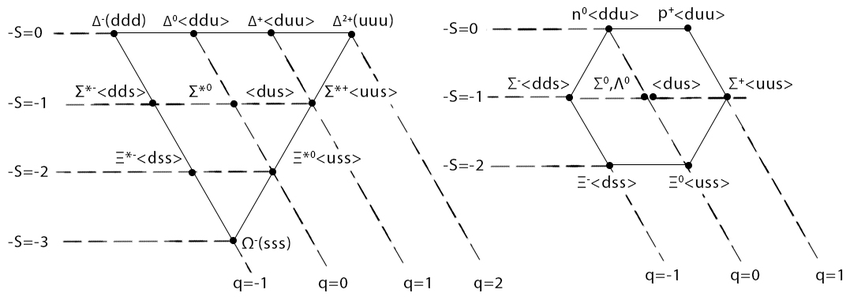
\includegraphics[width=0.8\linewidth]{Chapters/Introduction/Figs/eightfold_way.png}
\caption{Representation of the baryon decuplet (left) and octet (right) following the eightfold way approach for three kinds of quarks: up, down and strange. The horizontal levels represent the net strangeness number, while the diagonals (top left to bottom right) link baryons with the same electric charge.}
\label{fig:gelmann}
\end{center}
\end{figure}

They were later called quarks by Gell-Mann.
At a given point Gell-Mann and Zweig argued that, assuming the quarks' spin to be $1/2$, mesons could be explained as bound states of a quark and an antiquark, while baryons were a bound state of three quarks.
This choice lead to the peculiar electric charge of $\pm1/3$ and $\pm2/3$.
A last issue regarded the spin statistics theorem violation, solved by the introduction of an additional quantum number: the colour.
This was the birth of the quark model.
By assuming the hadronic matter is not fundamentally made of protons and neutrons they were able to organize in a elegant way the zoo of particles discovered during the $20^{th}$ century.

During the same years, Richard Feynman started thinking about a model useful for analyzing the hadrons produced in high energy physics experiments and capable of interpreting the radiation showers originating in ultra-relativistic collisions.
By introducing the partons and the parton distribution functions, Feynman was able to interpret the deep inelastic scattering on hadrons as the collision between the projectile and an inner constituent of the target, called parton \ref{fig:DIS}.

\begin{figure}[!ht]
\begin{center}
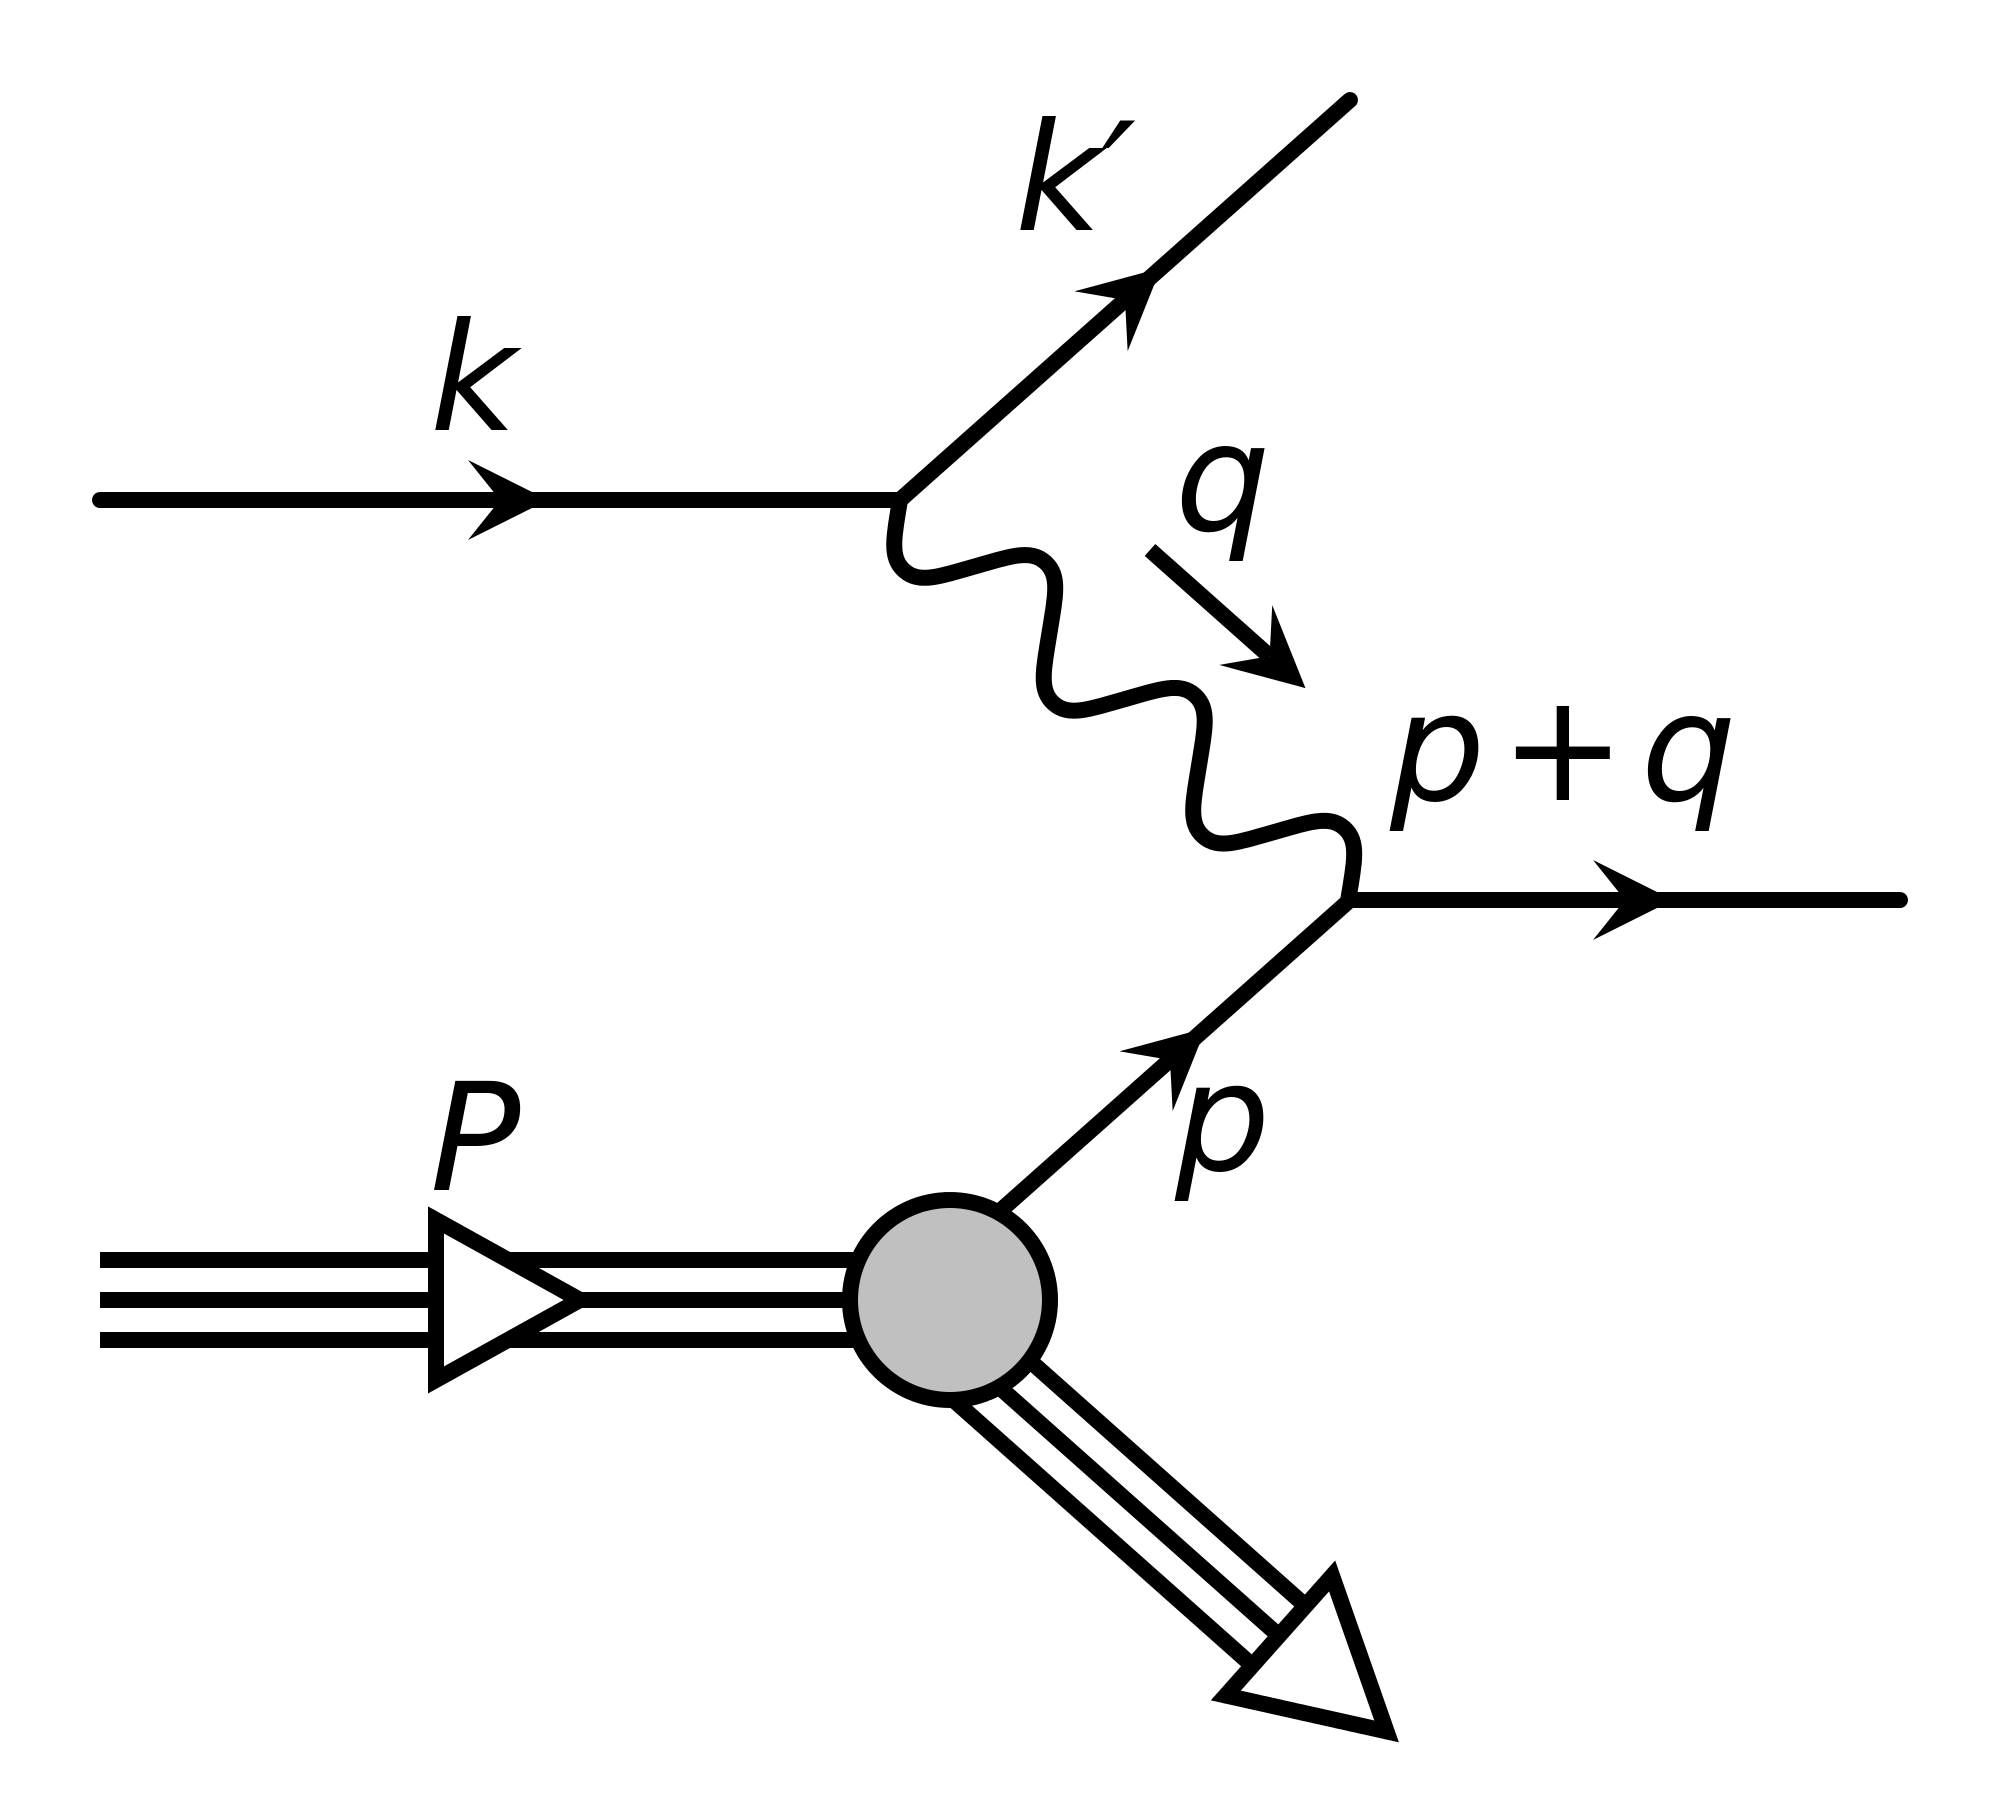
\includegraphics[width=0.5\linewidth]{Chapters/Introduction/Figs/DIS.png}
\caption{Cartoon of a deep inelastic scattering process between a projectile of momentum $k$ and $k'$and a parton of initial momentum $p$ belonging to a nucleon of initial momentum $P$. The interaction is mediated through the exchange of a boson of momentum $q$. The participant nucleons emerge from the interaction as an hadronic shower.}
\label{fig:DIS}
\end{center}
\end{figure}

Experiments of deep inelastic scattering performed at the Stanford Linear Accelerator Center (SLAC) between 1967 and 1973 pointed out a scaling behaviour, explained by Bjorken as a signature of the point like constituents of the proton.
Bjorken demonstrated that the functions which describe the structure of the nucleon neither depend on the transferred momentum ($Q^2$) nor on the energy transferred in the scattering ($\nu$), but on their ratio:

\begin{equation}
    x = \frac{Q^2}{2\cdot M \cdot \nu}
\end{equation}

The $x$ variable has no dimension and stands for the ration between the total momentum of the target and the fraction of that transported by the point-like constituent.


\begin{figure}[!t]
\begin{center}
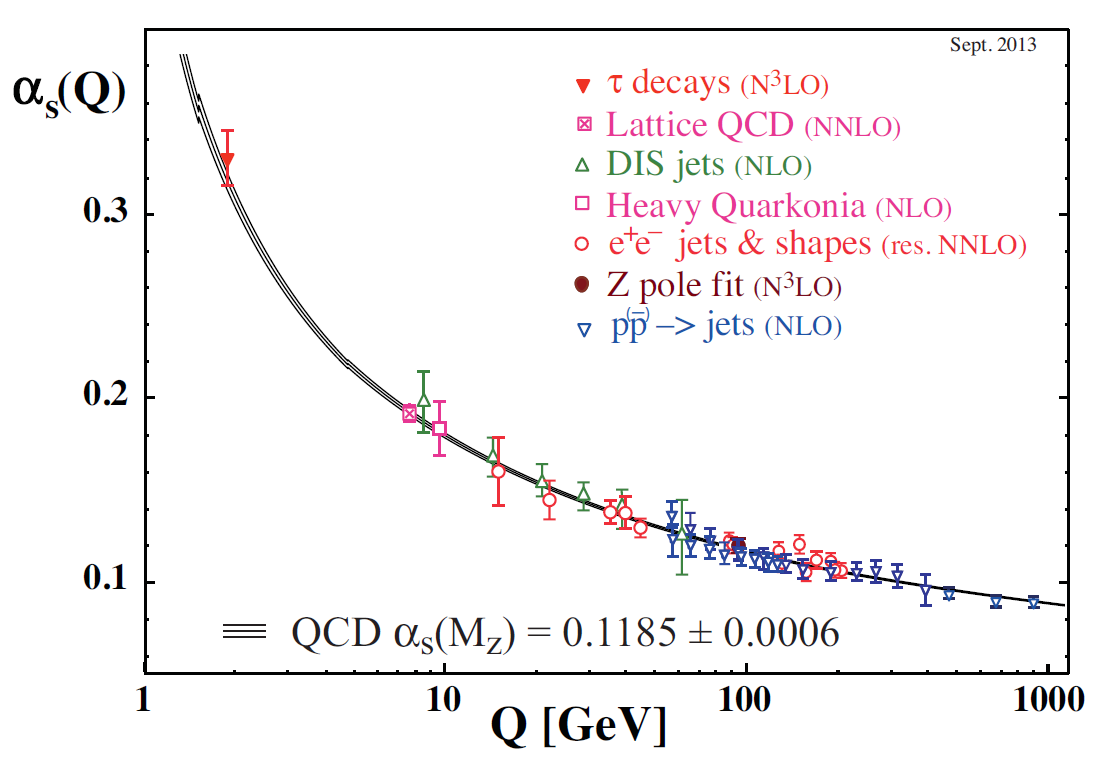
\includegraphics[width=0.85\linewidth]{Chapters/Introduction/Figs/QCD-running-coupling.png}
\caption{Plot of the running coupling constant of the strong interaction $\alpha_S$. The band has been computed using the standard model and several experimental points, obtained measuring the coupling from different processes, are shown.}
\label{fig:running}
\end{center}
\end{figure}

After few other proofs the Gell-Mann quarks and the Feynman partons turned out to be the same objects.
The answer to the first question was then well established (how are hadrons made?) when the physics community started tackling the second one regarding how do they interact.
The peculiarity of the new set of particles was the introduction of colour quantum number.
In 1973, in analogy with the Quantum Electro Dynamics (QED), the Quantum Chromo Dynamics (QCD) was proposed as the quantum field theory of the hadronic interaction.
The theory was supposed to be based on the existence of three colour charges and the non-Abelian simmetry group SU(3).
Eight massless generators represented the mediators of such interaction and were later called gluons.

The gluons are different with respect to the photons, since, as a effect of the non Abelian-ness of the theory, they carry a colour charge, making them auto interacting.
As a consequence the coupling constant of the strong interaction is defined as running, since it depends on the value of the transferred momentum $Q^2$\ref{fig:running}.
The running of the coupling constant leads to two peculiar proprieties, not found in any other fundamental interaction.
The strength of the interaction increases with distance.
This propriety leads to the confinement of quarks and gluons inside hadrons.

\begin{figure}[!t]
\begin{center}
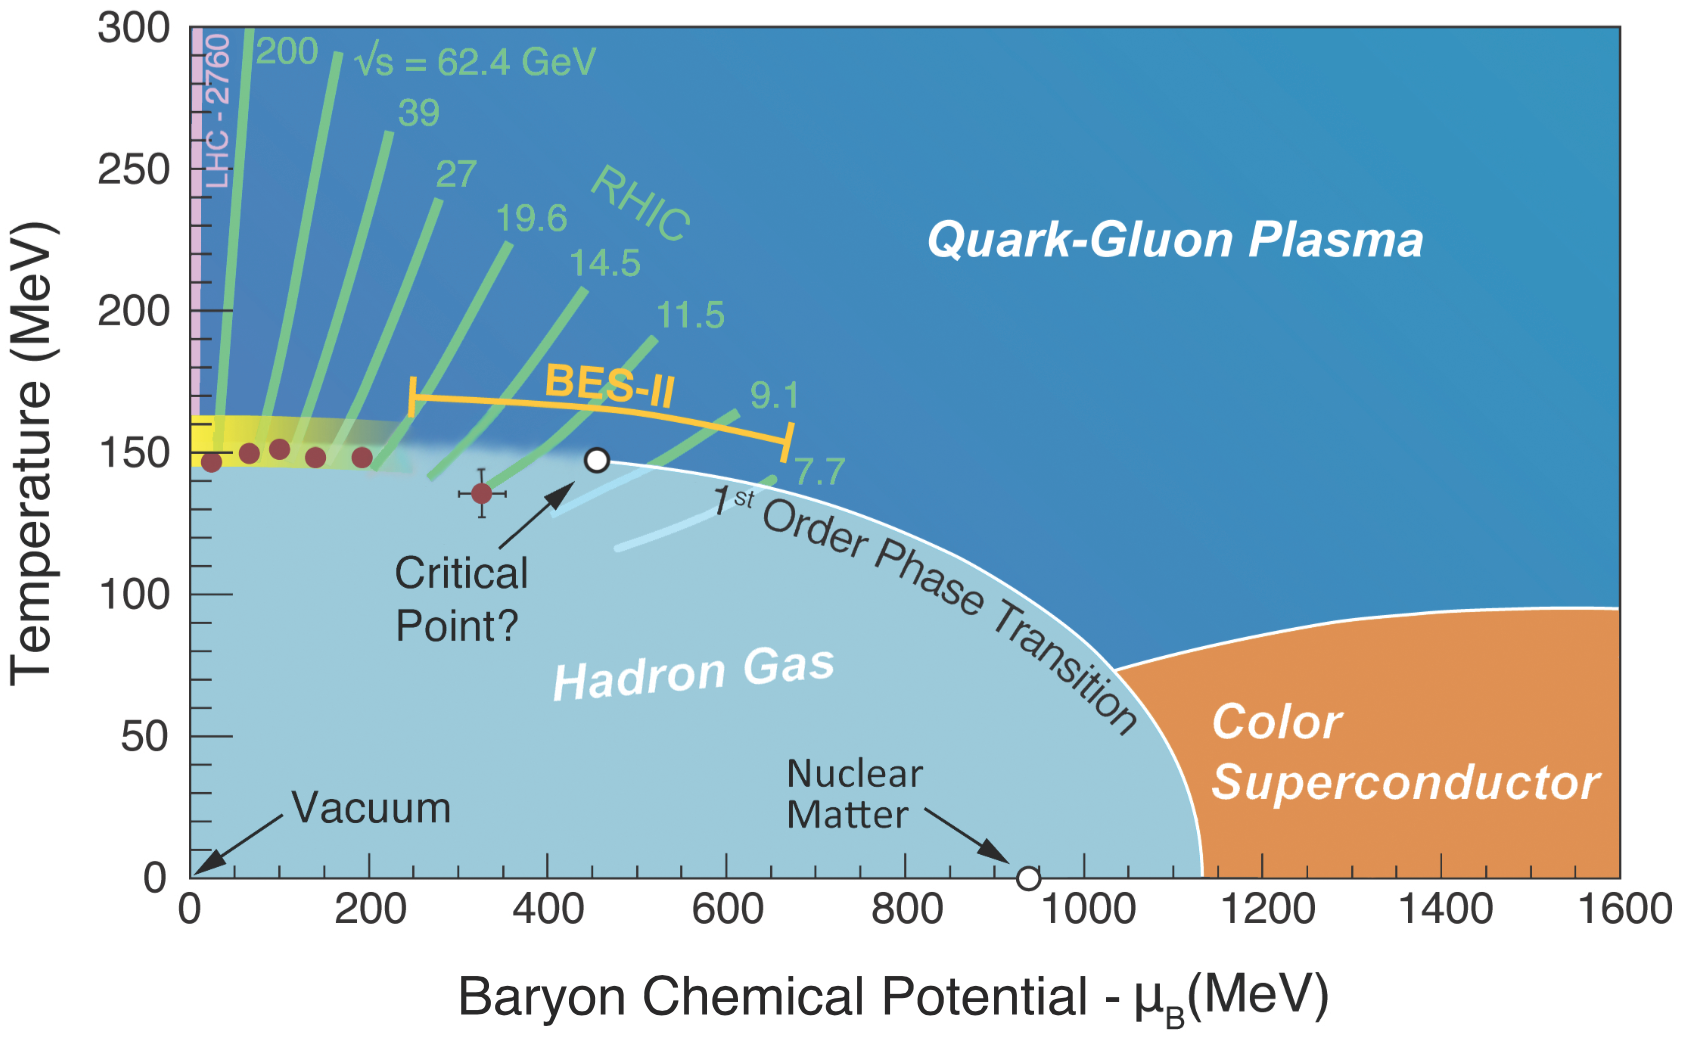
\includegraphics[width=0.85\linewidth]{Chapters/Introduction/Figs/QGPPhases.png}
\caption{Cartoon showing the main hadronic matter phases in a $(T,\mu_B)$ diagram.}
\label{fig:QGPPhases}
\end{center}
\end{figure}

\subsection{Quark Gluon Plasma}
In 1977 E. Shuryak coined the term Quark Gluon Plasma (QGP) to indicate a state of nuclear matter in which quarks and gluons are not confined anymore into hadrons.
From theoretical studies the main parameters determining the QGP evolution are the temperature (T) and the baryon-chemical potential ($\mu_B$), defined in a thermodynamical fashion as the differential of entropy with respect to the net baryon number.
Three main regions are spotted in the $(T,\mu_B)$ phase diagram \ref{fig:QGPPhases}:
\begin{itemize}
    \item At low T and low $\mu_B$ the nuclear matter is composed of hadrons behaving as a hadrons gas;
    \item At low T and high $\mu_B$ the nuclear matter degenerates to a gas of neutrons due to the collapse of hadronic structure. This state of nuclear matter is supposed to be present in the core of neutron stars;
    \item At high T and high $\mu_B$ the gas can be described as a gas of weakly interacting partons. Such behaviour is caused by the asymptotic freedom of QCD.
\end{itemize}
The extreme conditions needed for the QGP production are similar to the ones happened at the beginning of the universe evolution can be obtained in laboratory by means of ultra-relativistic heavy ion collisions.
According to the Big Bang model the conditions of high temperature and low baryon-chemical potential are supposed to be the ones of the early Universe.
At the beginning of the universe all the energy and matter were condensed in a tiny spatial region.
During the first microseconds of evolution, the universe started expanding from a condition of extreme energy density and temperature.
While expanding the energy density and the temperature started dropping.
Two transitions happened at $T\simeq160 MeV$ and $T\simeq100 KeV$: the hadron formation started at the first threshold, while small nuclei could survive after the second value.
The nuclear composition of early universe was fixed at that point: such phenomenon is called primordial nucleo-synthesis.
Only few minutes later, when the universe temperature dropped below $3000K$, the radiation decoupled from matter and the whole universe started becoming transparent.
The Cosmic Microwave Background (CMB) is the residual of the first radiation.

Studying the QGP evolution and its characteristics might lead to a better understanding not only of the strong nuclear interaction and the origin of hadrons masses, but also of the process of universe formation.

The best phenomenological model which can be cited to understand the artificial methodology to produce QGP is the bag model.
The two main hypotheses of this model are:
\begin{itemize}
    \item the quarks are massless particles put inside a bag of infinite dimension;
    \item the confinement originates from the balancing of the internal pressure exerted by quarks into the bag and an external pressure $B$;
\end{itemize}
The total energy of $N$ quarks confined in a spherical volume of radius $R$ is the sum of a kinetic term and a term related to the compensation by the external pressure $B$:
\begin{equation}
    E=\frac{2.04\cdot N}{R}\cdot \hslash c + \frac{4\pi}{3}\cdot R^3\cdot B
\end{equation}
The bag radius is determined by finding the minimum of energy of the system.
Such condition is obtained imposing the condition $dE/dR=0$.
\begin{equation}
\frac{dE}{dR}=-\frac{2.04\cdot N}{R^2}\cdot \hslash{h}c + 4\pi\cdot R^2\cdot B = 0
\end{equation}
The model allows one to compute confinement thresholds for various systems.
For example a baryon, composed by $N=3$ quarks and with $R=0.8 fm$ the external pressure becomes:
\begin{equation}
B^{1/4} = \frac{206 MeV}{\hslash c}
\end{equation}
Such value is the limit below which the confinement of the quarks inside the baryon happens.
If the internal pressure grows above such threshold the quarks start behaving as asymptotically free.
The internal pressure can increase in two ways:
\begin{itemize}
\item The increase of temperature causes an increase of kinetic energy of quarks inside the bag. In this situation the formed QGP is called "hot";
\item The increase of pressure is caused by the increase of baryon density achieved via compression. This scenario is possible in extremely dense objects such as neutron stars and is defined as "cold" QGP.
\end{itemize}

The heavy-ion collision experiments tackle the QGP production mainly trough the first approach, thank to the high energy available in the center of mass of the collision, while the use of heavy nuclei instead of light ones addresses the second method.
The bag model provides an estimation of the minimum temperature and energy density needed to produce the deconfined state.

The pressure required to produce a QGP out of a volume $V$ filled with massless quarks and gluons in which the net baryon number is null (equal number of quarks and anti-quarks) is computed as:
\begin{equation}
P = g_{tot}\cdot\frac{\pi^2}{90}\cdot T^4
\end{equation}
Where $g_{tot}$ is the total number of degrees of freedom for quarks, anti-quarks and gluons.
The pressure exceeds the external one at a temperature of around $145MeV$, a value similar to the lattice-QCD prediction of $160MeV$.
In addition, since the energy density is related to the pressure value, it can be computed as well:
\begin{equation}
\epsilon = 3\cdot P = g_{tot}\cdot\frac{\pi^2}{30}\cdot (160MeV)^4 \simeq 1 GeV/fm^3
\end{equation}
Which is considered to be the threshold value to produce a deconfined medium.

\begin{figure}[!ht]
\begin{center}
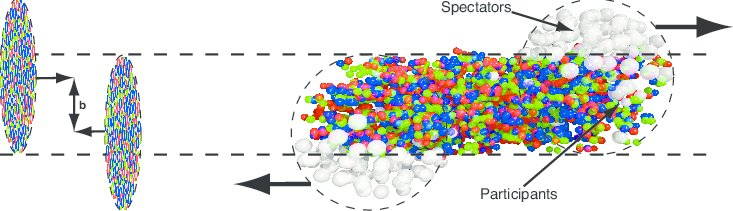
\includegraphics[width=0.99\linewidth]{Chapters/Introduction/Figs/collision.jpg}
\caption{Schematic of the stages on a heavy ion collision surrounding the collision moment. At first (left side) the nuclei are relativistically contracted. After the collision (right side) the spectators proceed unperturbed while the participants generate a colour tube filled of free partons.}
\label{fig:collision}
\end{center}
\end{figure}

The computed threshold can be crossed in ultra-relativistic heavy ion collisions
Such kind of collision involves a variable number of nucleons depending on the centrality of the collision.
The collision process is characterized by a complex space and time envelop, but can be divide in some macro-conditions which can help understanding the whole process \ref{fig:evolution}:
\begin{itemize}
    \item Before the collision the nuclei are Lorentz-contracted \ref{fig:collision}. The transverse spatial separation between the centroids of the two nuclei is called impact parameter and determines the number of nucleons participating to the interaction;
    \item at $t=0$ the collisions process starts and all the available energy is concentrated in the central region;
    \item Right after the collision the central "fireball" starts expanding following pressure gradients. The partons act as deconfined during this phase. The conservation of energy causes the temperature to drop depending on the fireball expansion;
    \item The chemical freeze-out happens when the average temperature drops below a threshold which at LHC amounts to $\simeq160 MeV$. The energy of the interactions does not allow to modify the abundances of hadrons;
    \item The thermal freeze-out corresponds to the moment in which the elastic interactions between hadrons stop.. At this point the kinematic spectra of the produced hadrons is fixed. The threshold temperature for this situation has be computed to be around $120 MeV$.
\end{itemize}

\begin{figure}[!t]
\begin{center}
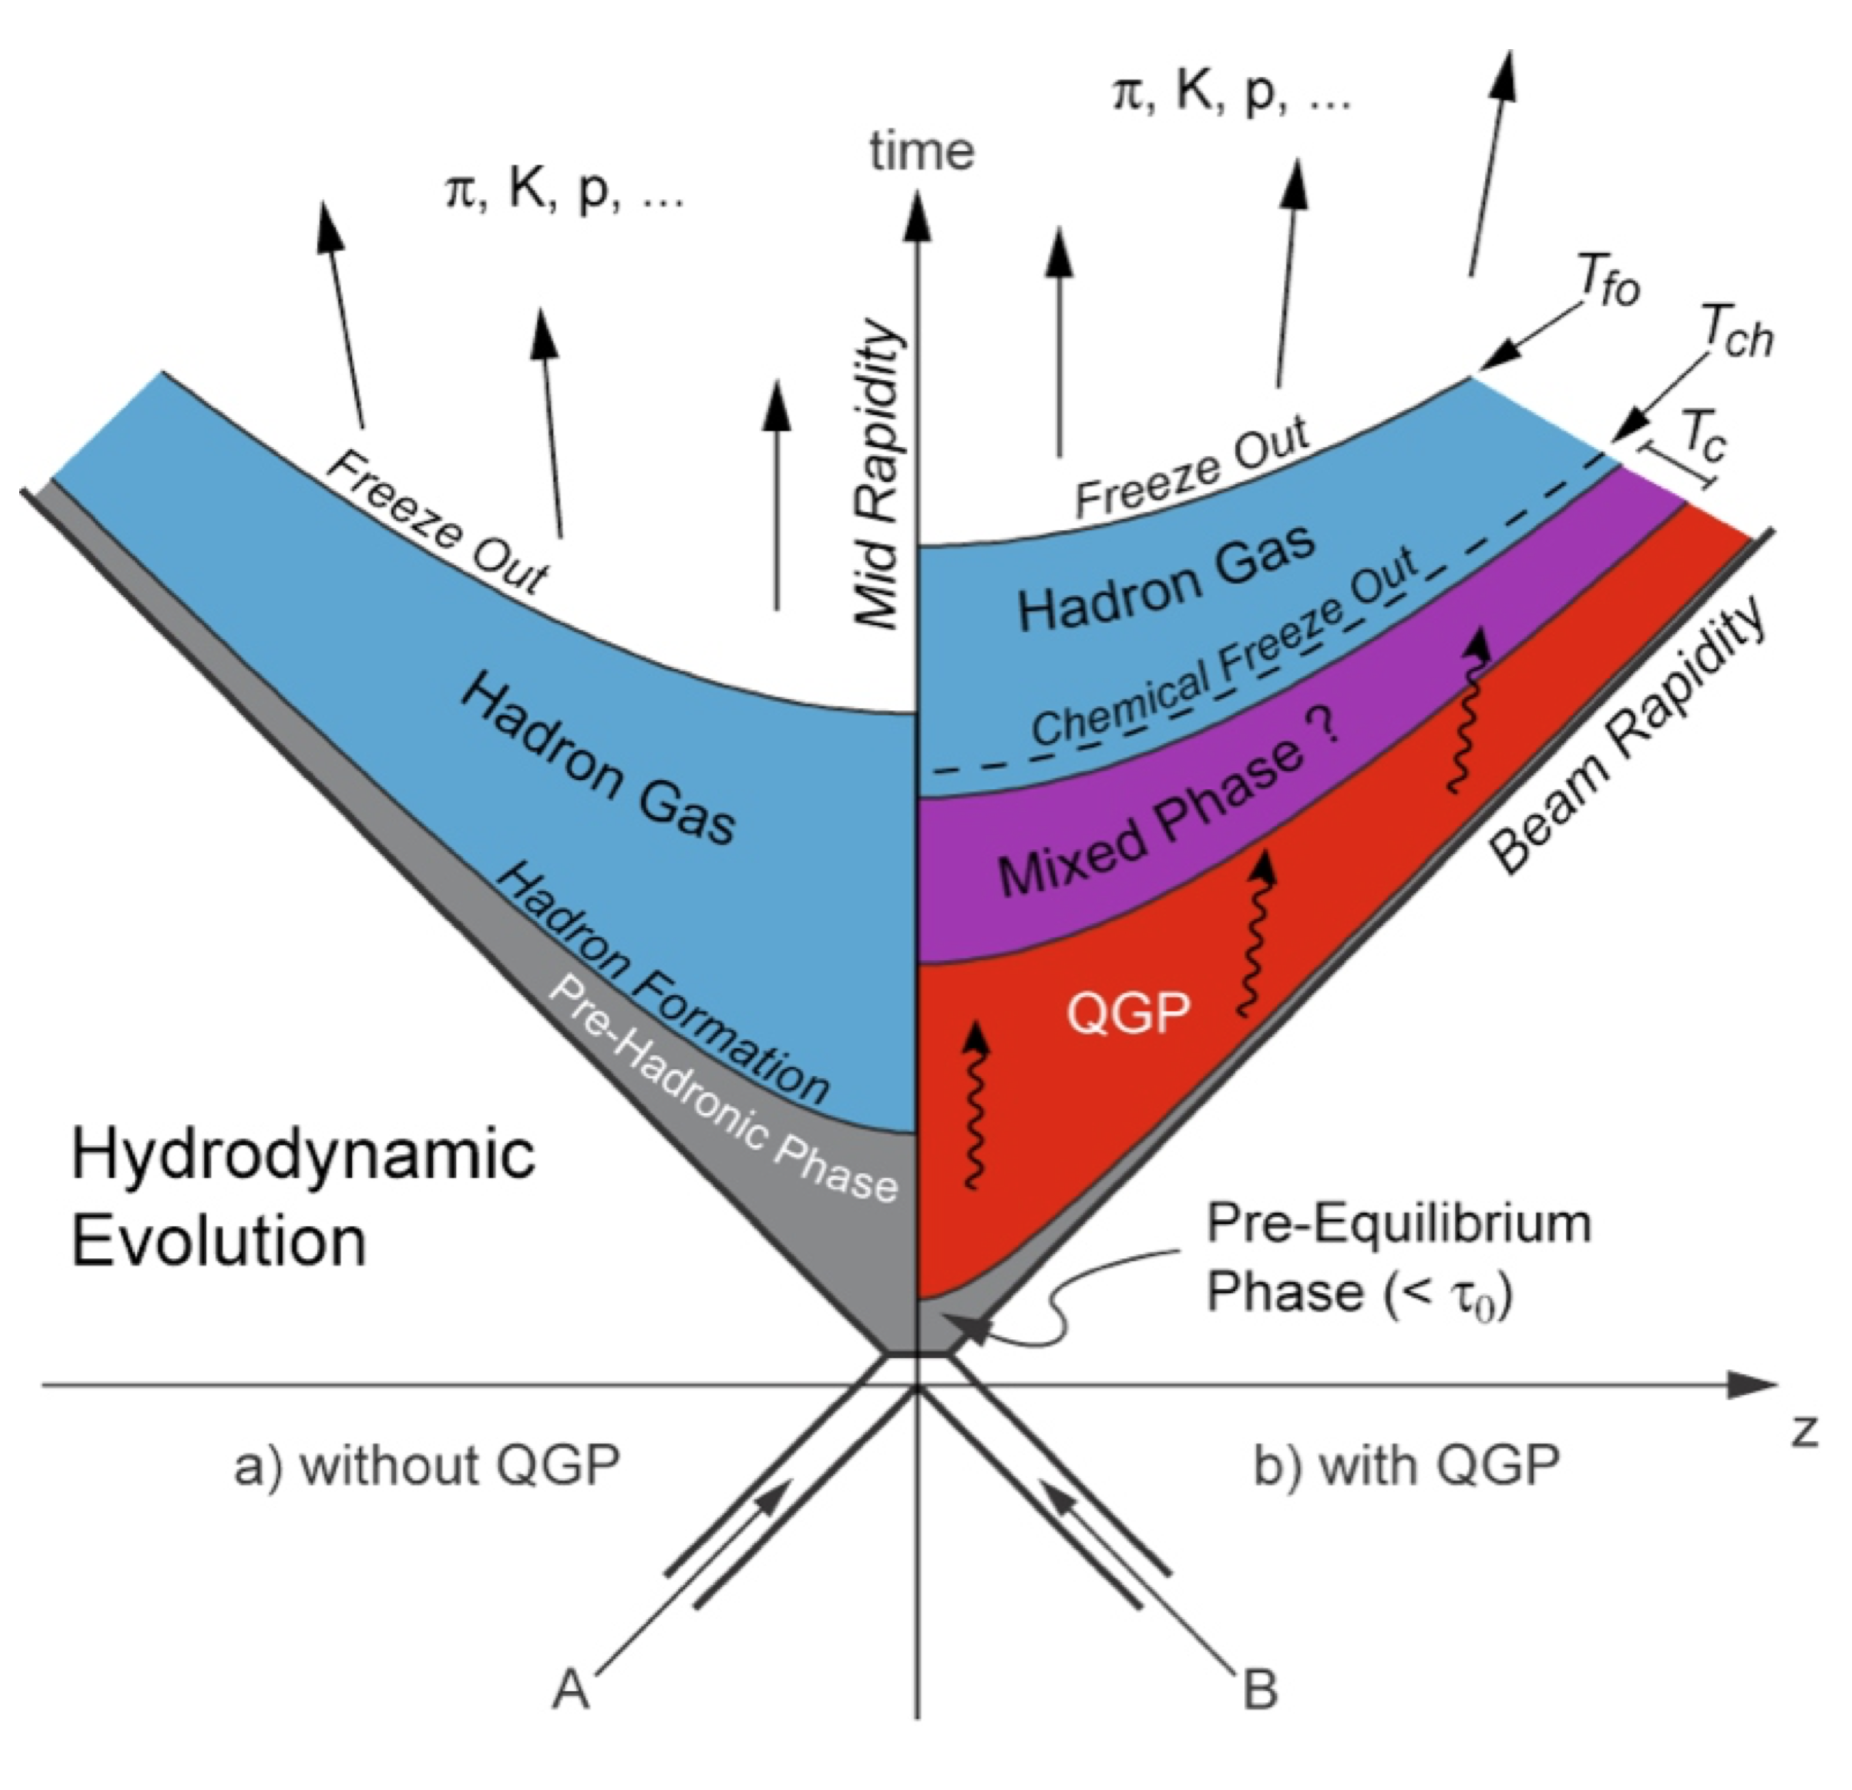
\includegraphics[width=0.85\linewidth]{Chapters/Introduction/Figs/QGP_evo.png}
\caption{Space-time evolution of the fireball originated from an heavy ion collision with (left) and without (right) QGP.}
\label{fig:evolution}
\end{center}
\end{figure}

The QGP phase is extremely short-lived and a direct observation is impossible.
However, after the thermal freeze-out the hadrons fly freely and they can be detected by the experiment.
This argument lead to the idea of studying the QGP by analyzing the emerging particles.
In fact emerging hadrons and particles which have been influenced by QGP formation, might bring some important information regarding its characteristics.

\subsection{Soft and hard probes}
The particles produced in a nuclear collision might be distinguished in soft and hard probes.
Soft probes are produced during the evolution of the system formed in the collision and are related to the collective behaviour of the medium.
The processes involving a soft probe production are characterized by low transferred momentum and for this reason $99.5\%$ of the produced particles are soft probes.
Some examples of soft probes are:
\begin{itemize}
    \item Particle multiplicity: the multiplicity of particles produced is important for the determi- nation of the energy density of the collision and the study of their transverse momentum spectra allows to obtain information on the chemical and thermal freeze-out;
    \item Collective flow: the spatial anisotropy of the colliding region induces pressure gradients which cause anisotropic particle distributions. This effect can be explained as a collective motion of particles produced in the interaction and its study is closely related to the determination of the equation of state for a deconfined medium;
    \item the study of these electromagnetic probes is important for the determination of the medium temperature.
\end{itemize}
By contrast to soft probes, hard probes are particles produced in high transferred momentum processes and they are characterized by much lower production cross section.
For this reason hard probes are produced early during the collision and can be strongly influenced by a deconfined medium.
Some examples of hard probes are:
\begin{itemize}
    \item Jet quenching: jets are produced by the fragmentation of high momentum partons. Inter- acting with a deconfined medium they can lose energy scattering with other free partons or through radiative gluon emission. The result is a quenched particle spectrum;
    \item heavy flavour multiplicity: states characterized by the presence of heavy quarks (charm or bottom) are very important in the study of QGP, especially via energy loss processes into a deconfined medium;
    \item Quarkonium production modification: the term quarkonium indicates a bound state of two heavy quarks and it is named charmonium when formed by charm quarks, bottomomium when formed by bottom quarks. These mesons are strongly affected by the formation of a partonic medium and this effect can result in a suppression due to a mechanism of color screening.
\end{itemize}

The bottomonium studied in the analysis chapter of this thesis belongs to the set of hard probes studied by ALICE.

\subsection{Centrality estimation: Glauber's model}\label{intro_glauber}
It is commonly known that nuclei are non poin-like objects.
Since each nucleon brings a part of the total nucleus momentum, the impact parameter of a nuclear collision determines the number of participant nucleons, hence the amount of available energy in the center of mass.
The measurement of the impact parameter is fundamental to know the nature of the initial collision state.
Glauber's model is the approximation usually used to model and analyze a nuclear collision characteristics, named after Roy Glauber.
The model stands on three basic assumptions:
\begin{itemize}
\item At high energy the nucleons are undeflected thanks to the large momentum, hence their trajectory is asymptotically linear;
\item Nuclear size has to be large compared to the range on nucleon-nucleon interaction;
\item Nucleons' motion independent from the nucleus one, hence the nuclear collision can be described in terms of the nucleon-nucleon cross section.
\end{itemize}

As one can already argue, the Glauber's approach to the description of nuclear collisions simplifies the problem diving to a more fundamental description, given at the nucleon level.
For doing so two inputs are necessary:
\begin{itemize}
\item Inelastic nucleon-nucleon cross section. 
This value should be measured at the same center-of-mass energy. 
It can be measured in proton-proton collisions;
\item Nucleus density profile. It is necessary to provide a contour shape for the colliding nuclei. 
Historically the nucleus profile has been modeled in the shell model approach as a Woods-Saxon distribution, which models the average nucleon potential in the nucleus. 
The potential shape corresponds to the nucleons distribution.
The Woods-Saxon distribution is represented in figure \ref{fig:WoodsSaxon} for a $Pb$ nucleus and presented in equation \ref{eq:WoodsSaxon}, where:
\begin{itemize}
\item $r$ is the radial position at which one wants to compute the nucleons density;
\item $\rho_0$ is the density value at $r=0$;
\item $\omega$ is a parameter which can represent a density bump right before the distribution tail;
\item $R$ is the radius at which $\rho/\rho_0=50\%$, similar to a half-width half maximum;
\item $a$ describes the steepness of the distribution's tail.
\end{itemize}
The Woods-Saxon distribution parameters are typically determined via $e^-$-nucleus scattering processes.
The differences between protons and neutrons are assumed to be negligible.

\begin{equation}
\label{eq:WoodsSaxon}
\rho(r) = \frac{\rho_0\cdot(1+\omega r^2/R^2)}{1+\exp(\frac{r-R}{a})}
\end{equation}

\end{itemize}

\begin{figure}[!t]
\begin{center}
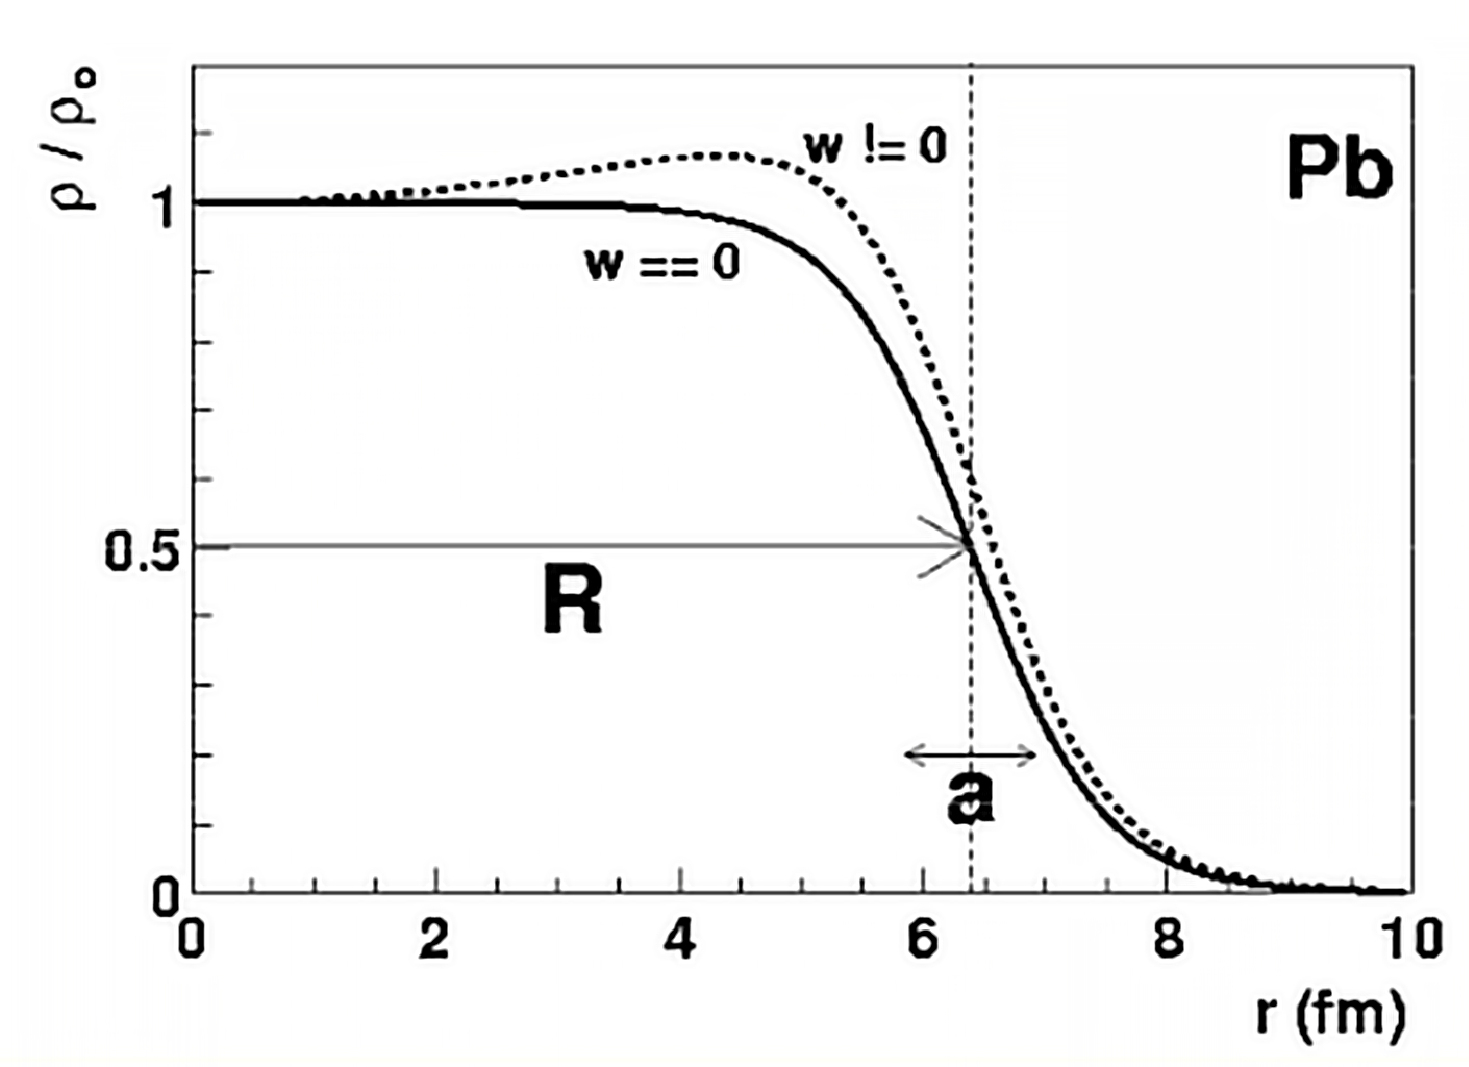
\includegraphics[width=0.7\linewidth]{Chapters/Analysis/Figs/woods-saxon.pdf}
\caption{Woods-Saxon potential for $Pb$ nucleus as the ration of the $\rho(r)$ over $\rho_0$ as a function of the distance from the nucleus center ($r$).
Displayed parameters are extensively described in paragraph \ref{intro_glauber}}
\label{fig:WoodsSaxon}
\end{center}
\end{figure}

\begin{figure}[!t]
\begin{center}
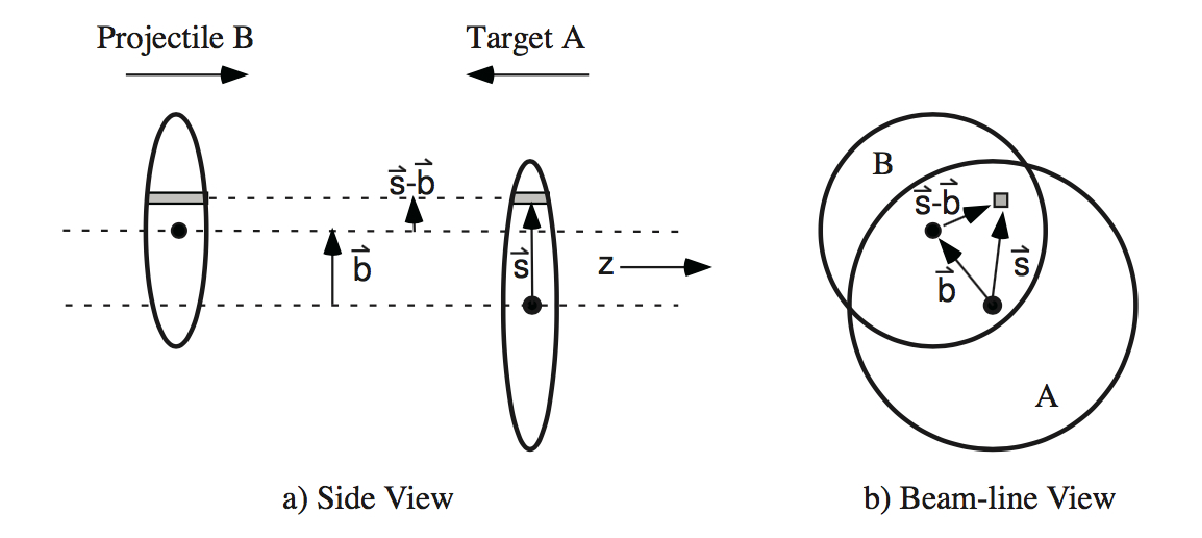
\includegraphics[width=0.85\linewidth]{Chapters/Analysis/Figs/glauber-side.pdf}
\caption{Schematic representation of the Optical Glauber Model geometry, with transverse (a) and longitudinal (b) views. From \cite{Miller:2007ri}.}
\label{fig:GlauberSide}
\end{center}
\end{figure}

The Glauber's model uses an optical and geometric approach to represent the nuclear collision.
Referring to picture \ref{fig:GlauberSide}:
\begin{itemize}
\item $b$ is the distance between the centers of the colliding nuclei, namely the impact parameter;
\item $s$ is the distance of a nucleon flux tube relative to the nucleus center.
\end{itemize}
Note that in this discussion the vectors $\vec{b}$ and $\vec{s}$ will be replaced by their modulus.
This can be done if the colliding particles are not polarized and present a spherical distribution of probability for the nucleon density.
This assumption is legitimate for Pb nuclei.

The probability of finding a nucleon in a nucleon flux tube posed at $s$ from target A is defined in equation \ref{eq:TAs}.
The same equation can be rephrased to compute the same probability for the projectile, namely B.

\begin{equation}
\label{eq:TAs}
\hat{T}_A(s) = \int\hat{\rho}_A(s,z_A)dz_a
\end{equation}

The effective overlap area of two specific nucleons can be described by the equation \ref{eq:TAB}, in which the definition introduced in \ref{eq:TAs} is extensively adopted.
$\hat{T}_{AB}(\vec{b})$ dimension is an inverse area.

\begin{equation}
\label{eq:TAB}
\hat{T}_{AB}(b) = \int\hat{T}_A(s)\hat{T}_B(s-b)d^2s
\end{equation}

The probability of inelastic interaction between two specific nucleons belonging to A and B respectively can be described by equation \ref{eq:PAB}.

\begin{equation}
\label{eq:PAB}
P_{AB}(b)=\hat{T}_{AB}(b)\sigma_{inel}^{NN}
\end{equation}

Since the nucleons in A and B are not distinguishable, this interaction probability has to be reworked in order to loose the attribute of being specific for two nucleons.
Using a binomial distribution of probability one obtains \ref{eq:Pnb}, where $AB$ is the product of the number of nucleons and $n$ in the number of desired nucleon-nucleon collisions.

\begin{equation}
\label{eq:Pnb}
P(n,b)=\binom{AB}{n}[P_{AB}(b)]^n[1-P_{AB}(b)]^{AB-n}
\end{equation}

Using the last equation, defining:
\begin{itemize}
\item Collision: a nucleon-nucleon collision;
\item Participant: a nucleon which takes part to at least one nucleon-nucleon collision;
\item Spectator: a nucleon which doesn't take part to any collision.
\end{itemize}
one can compute $N_{coll}(\vec{b})$ (number of nucleon-nucleon collisions), $N_{part}(\vec{b})$ (number of participant nucleons) and $N_{spec}(\vec{b})$ (number of spectator nucleons).

\begin{equation}
\label{eq:Ncoll}
N_{coll}(b)=\sum_{n=1}^{AB}nP(n,b)=AB\hat{T}_{AB}(b)P_{AB}(b)
\end{equation}

\begin{equation}
\label{eq:Npart}
N_{part}(b)=A\int\hat{T}_A(s){1-[1-P_{AB}(s-b)]}d^2s + B\int\hat{T}_A(s-b){1-[1-P_{AB}(s)]}d^2s
\end{equation}

\begin{equation}
\label{eq:Nspec}
N_{spec}(b)=A+B-N_{part}(b)
\end{equation}

In figure \ref{fig:GlauberAuAu} participants of a $Au--Au$ collision are shown in strong blue and red, while semi-transparent blue and red dots represent the spectators.

\begin{figure}[!t]
\begin{center}
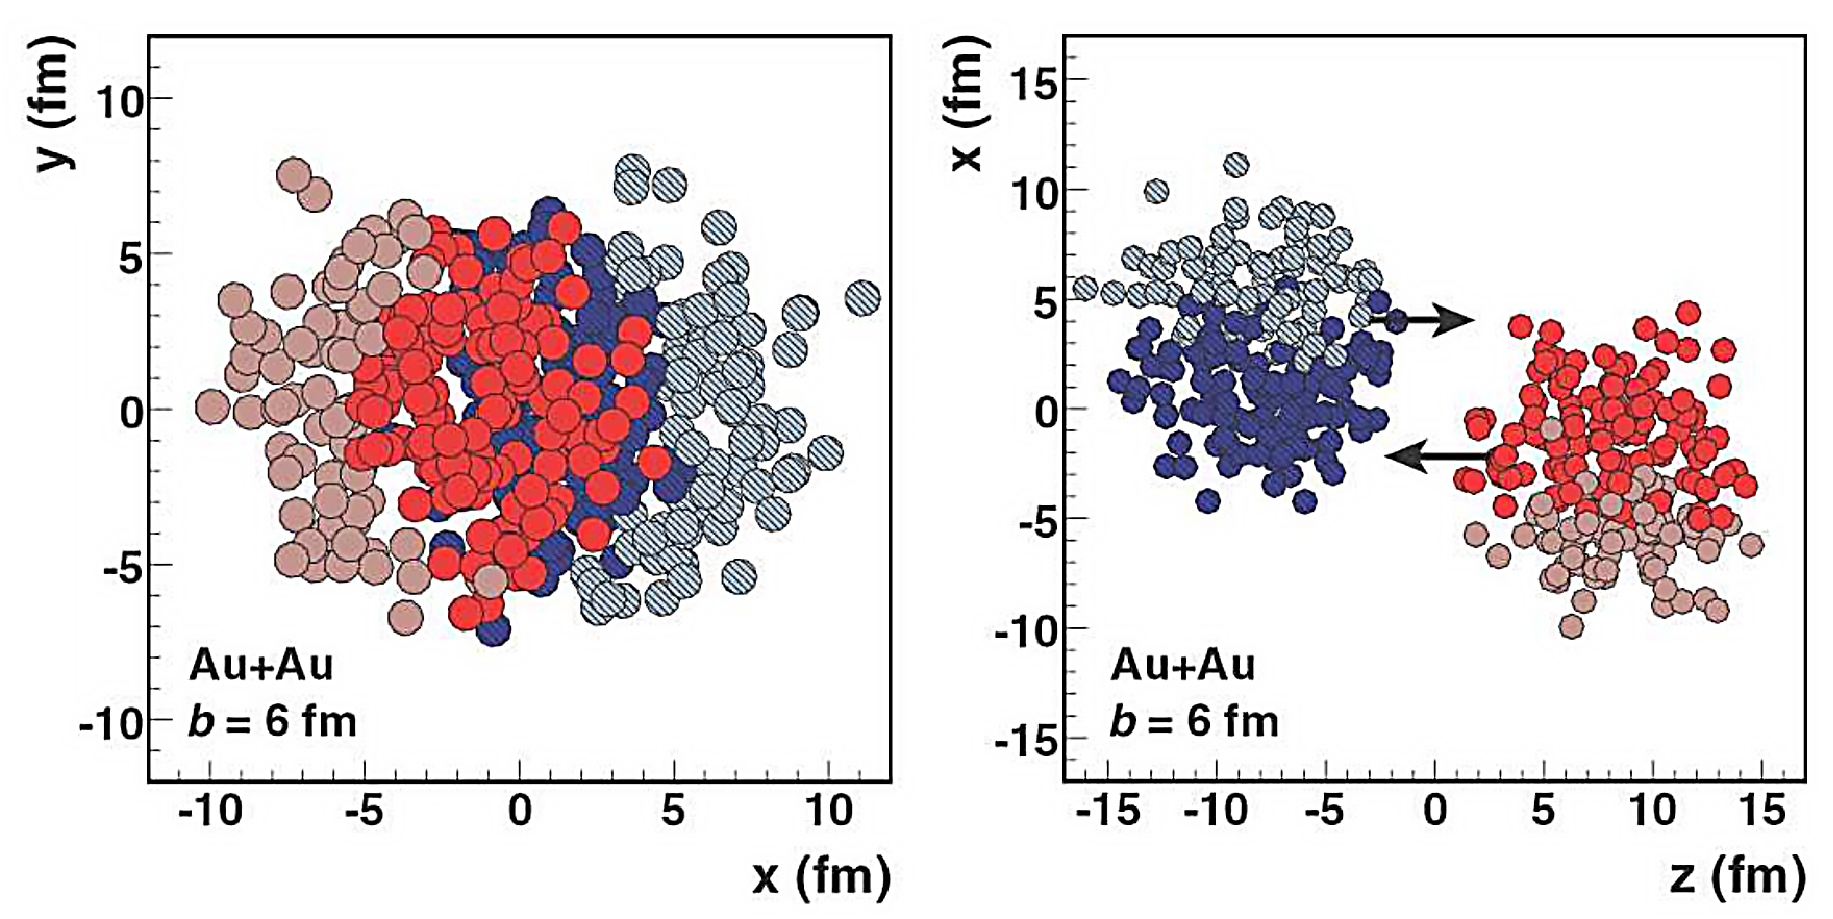
\includegraphics[width=0.9\linewidth]{Chapters/Analysis/Figs/glauber-pbpb.pdf}
\caption{Glauber Monte Carlo $Au--Au$ collision with impact parameter $b=6 fm$ seen in the trasverse plane (left) and along the beam axis (right). Nucleons area is equal to $\sigma_{inel}^{NN}$. From \cite{Miller:2007ri}.}
\label{fig:GlauberAuAu}
\end{center}
\end{figure}

Through the Glauber's model a measurement of the number of participant or spectator nucleons can provide an indirect measurement of the impact parameter of a nuclear collision.
Unfortunately neither $N_{part}(b)$ nor $N_{spec}(b)$ can be directly measured.
Typically the number of participants is related to the charged particles multiplicity ($N_{ch}$).
$N_{ch}$ has been measured over a large range of rapidity and is well described by a negative binomial distribution \cite{Aamodt:2009aa}.
This approach allows to simulate an experimental multiplicity distribution that can then be linked to an experimental observable.
In figure \ref{fig:GlauberCent} the collision probability is represented as a function of $N_{ch}$. Additional axes represent the correlation between centrality and $N_{part}$, $b$ and fraction of the total cross section $\sigma/\sigma_{tot}$.
For ALICE one of the detectors, the VZERO, provides a signal whose amplitude is the $N_{ch}$ estimation provider, hence the source of the main centrality evaluation, as shown in picture \ref{fig:GlauberVZERO}.


\begin{figure}[!t]
\begin{center}
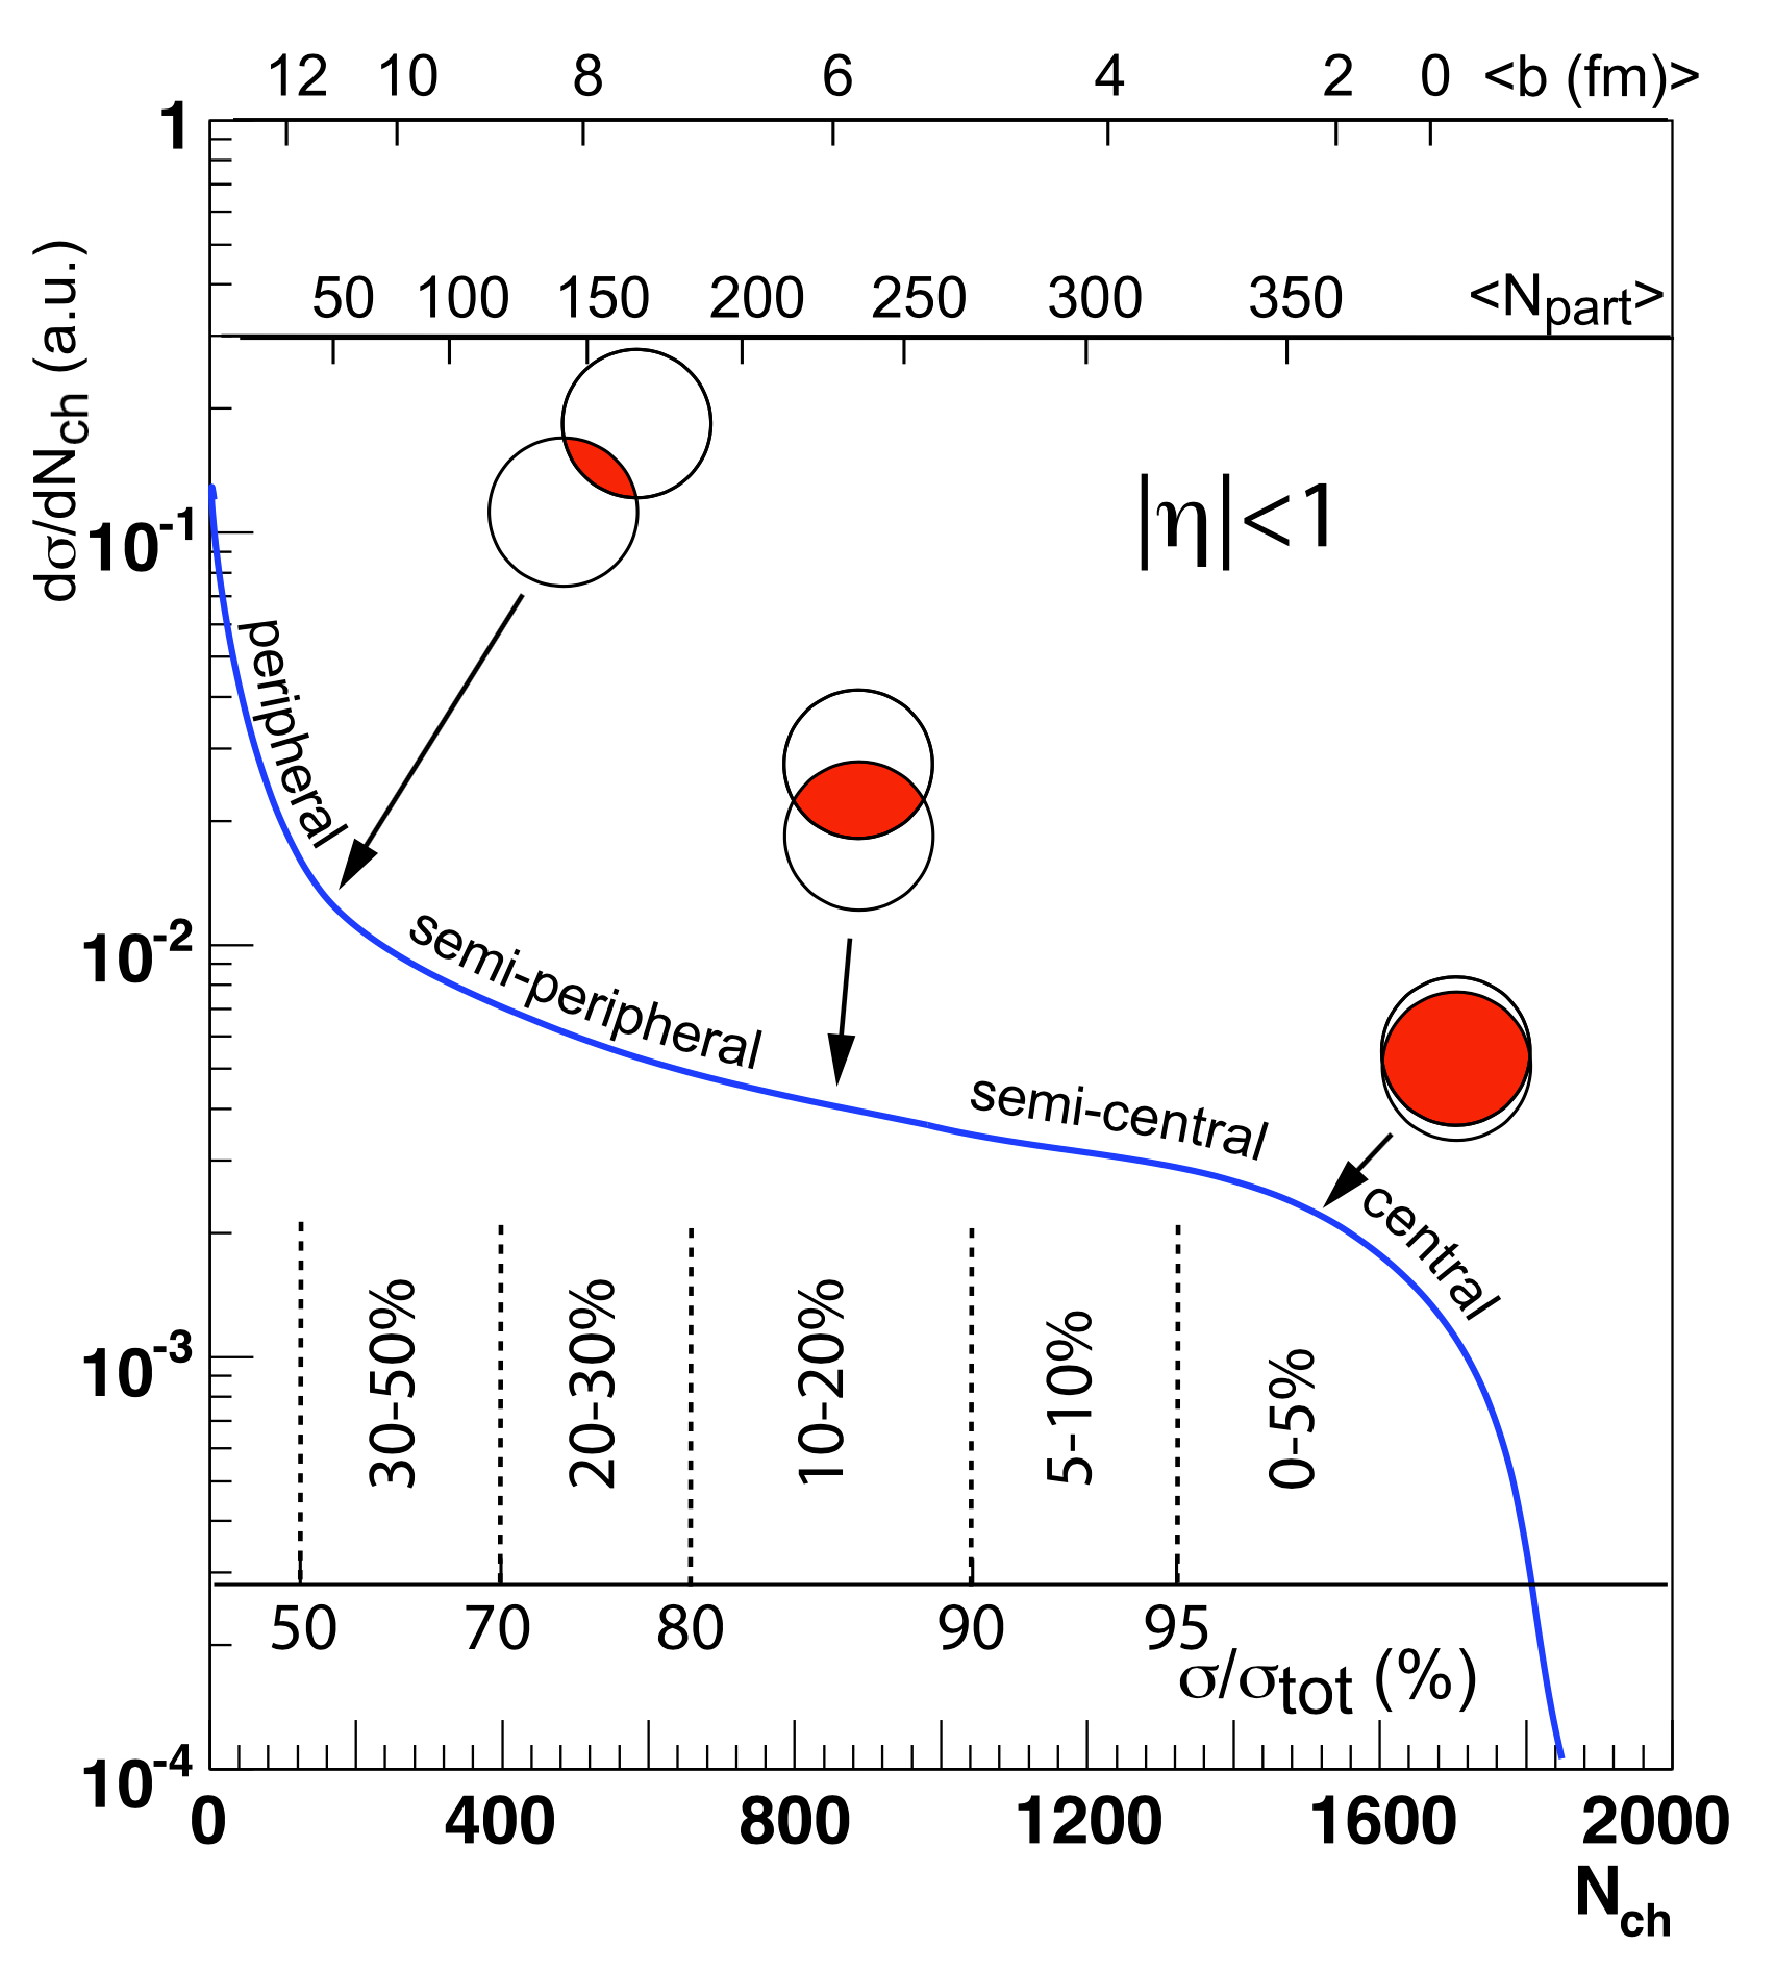
\includegraphics[width=0.75\linewidth]{Chapters/Analysis/Figs/glauber-centrality.pdf}
\caption{A cartoon example of the correlation of the final state observable $N_{ch}$ with Glauber calculated quantities ($b$, $N_{part}$). The plotted distribution and various values are illustrative and not actual measurements. From \cite{Miller:2007ri}.}
\label{fig:GlauberCent}
\end{center}
\end{figure}

\begin{figure}[!t]
\begin{center}
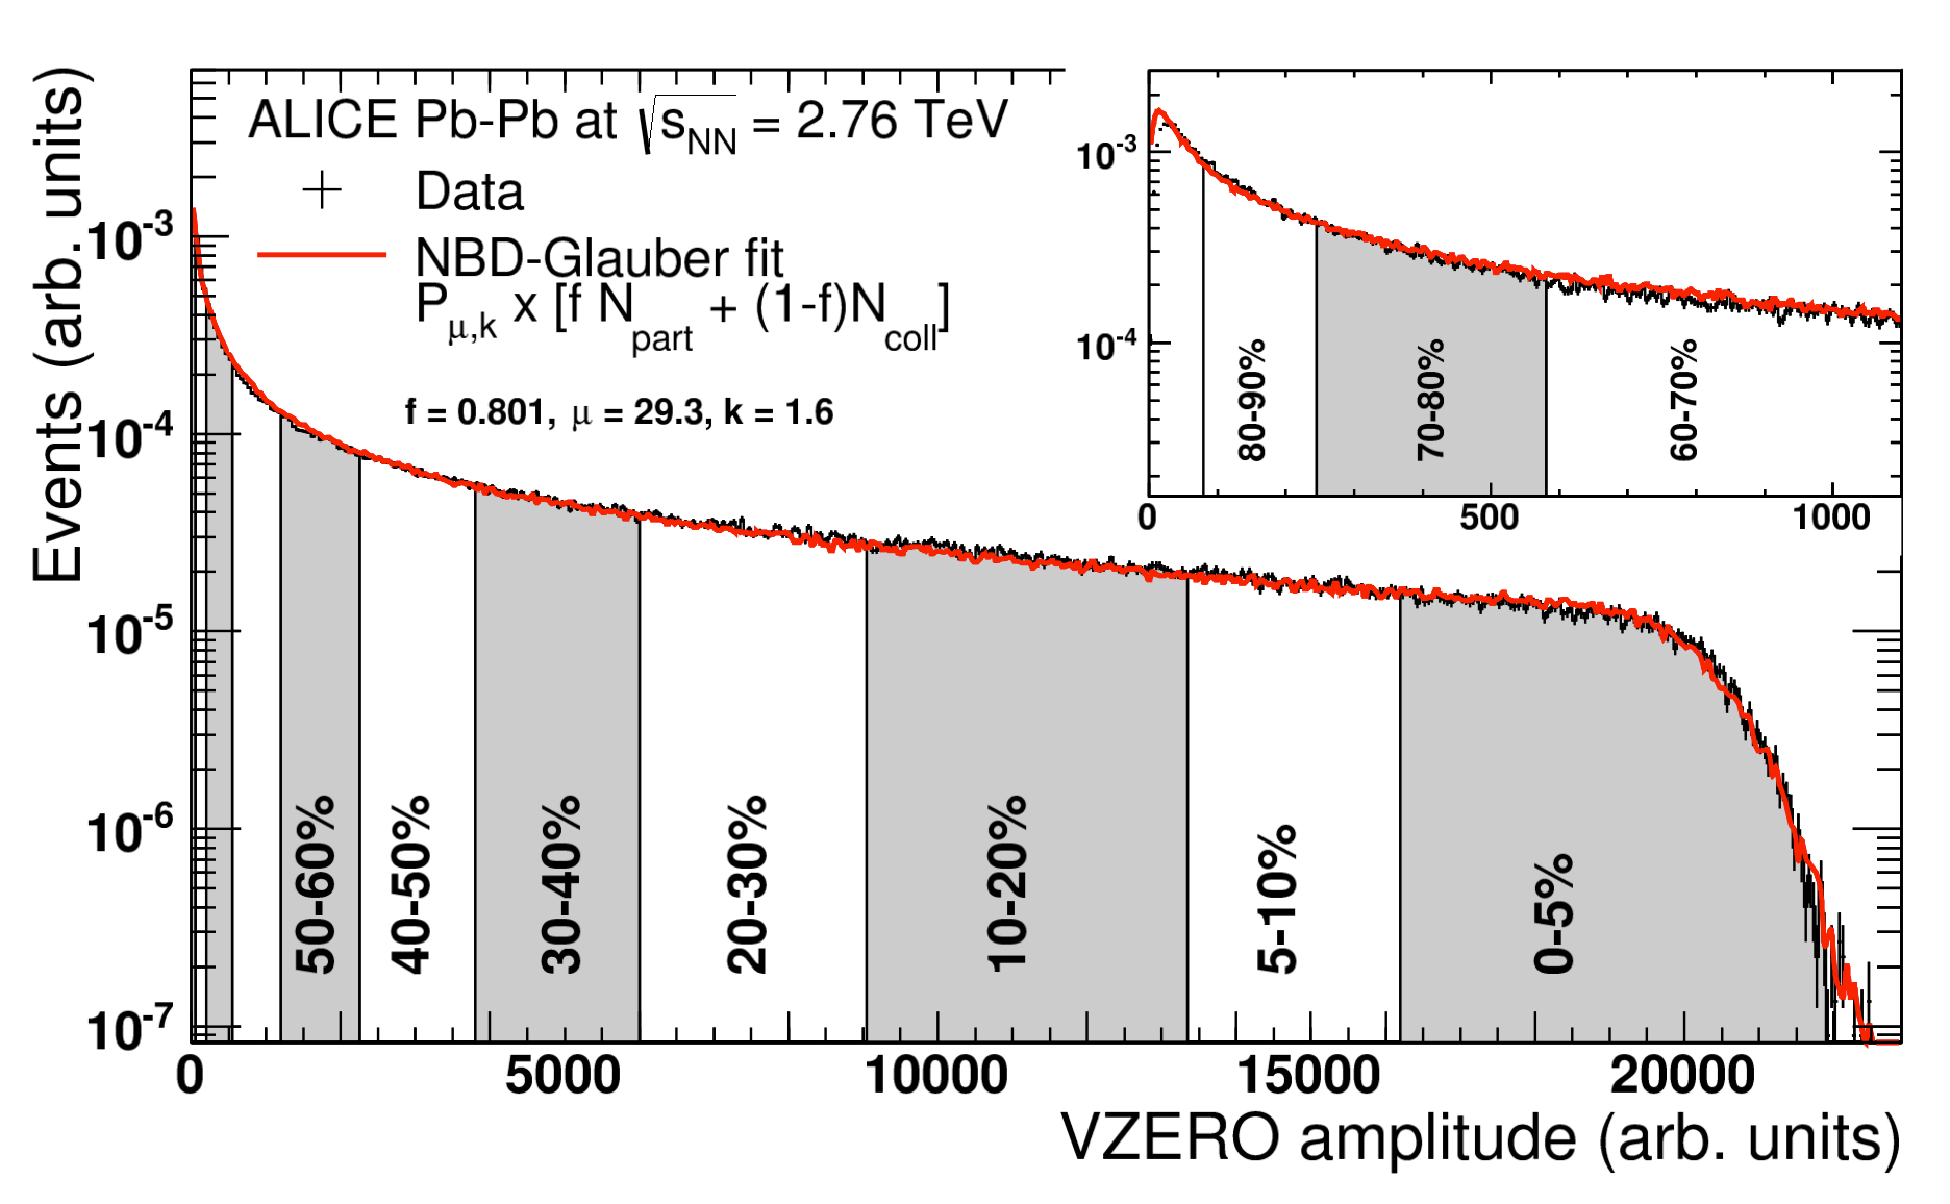
\includegraphics[width=0.85\linewidth]{Chapters/Analysis/Figs/glauber-vzero.pdf}
\caption{Distribution of the sum of amplitudes in the VZERO scintillators. The distribution is fitted with the NBD-Glauber fit shown as a red line. The centrality classes used in the analysis are indicated in the figure. The inset shows a zoom of the most peripheral region. From \cite{Abelev:2013qoq}.}
\label{fig:GlauberVZERO}
\end{center}
\end{figure}

\subsection{Nuclear modification factor}\label{RAA}
In general the study of the modifications of the production of probes in heavy nuclei collisions, with respect to proton--proton collisions, makes use of the nuclear modification factor definition.
The definition of the nuclear modification factor follows the Glauber's approach, using its model observables to obtain a centrality-dependent form.
The simplest mathematical form of the nuclear modification factor is the one reported in \ref{eq:RAA}.

\begin{equation}[!t]
\label{eq:RAA}
R_{\rm{AA}}^X = \frac{N_{\rm{AA}}^X}{<N_{coll}>\cdot N_{\rm{pp}}^X}
\end{equation}

Where $R_{\rm{AA}}^X$ is the nuclear modification factor for the species $X$, $<N_{coll}>$ is the number of binary nucleon--nucleon collisions happening in the nucleus--nucleus collision and $N_{\rm{(pp,AA)}}^X$ are the yields of $X$ states in a proton--proton and a nucleus--nucleus collision, respectively.
The formulation of the denominator of the fraction defining the $R_{\rm{AA}}^X$ originates from the assumption that nucleons in a nucleus behave as an incoherent superposition of $A$ nucleons.
To simplify, the denominator corresponds to the number of $X$s one would be able to measure in the case in which the binding between nucleons in the nuclei would have no effect on the single binary collision.
Moreover the denominator formulation models that during each binary collision the spectator nucleons are neither participating nor perturbing the binary collision outcome.
The meaning of $R_{\rm{AA}}^X$ is then trivial: it represents the deviation from the "ideal" situation in which mutual interactions between nucleons have no visible effect of the yields of a nucleus--nucleus collision.

\begin{equation}
\label{eq:yields}
N_{\rm{pp}}^X = \frac{\sigma_{\rm{pp}^{X}}}{\sigma_{\rm{pp}_{MB}}}
\end{equation}

The yields of a given state $X$ can be defined using its cross-section. The definition reported in \ref{eq:yields} can be then introduced in \ref{eq:RAA} giving a definition of the nuclear modification factor which is more suitable for substitution with measurements. This substitution can be rewritten using the Glauber's model definition of nuclear overlap factor as in equation \ref{eq:TAA}, leading to \ref{eq:RAA2}.

\begin{equation}
\label{eq:TAA}
T_{\rm{AA}} = \frac{<N_{coll}>}{\sigma_{\rm{pp}_{MB}}}
\end{equation}

\begin{equation}
\label{eq:RAA2}
R_{\rm{AA}}^X = \frac{N_{\rm{AA}}^X}{T_{\rm{AA}} \cdot \sigma_{\rm{pp}}^X}
\end{equation}

For the nuclear modification factor three scenarios can be foreseen for the nuclear modification factor values:
\begin{itemize}
\item $R_{\rm{AA}}^X<1$: a nucleus--nucleus collision presents a net suppression of the production of $X$s;
\item $R_{\rm{AA}}^X>1$: during the nucleus--nucleus collision a net enhancement of the production of $X$s is observed; 
\item $R_{\rm{AA}}^X=1$: the nucleus--nucleus collision can be interpreted as an incoherent superposition of binary nucleon--nucleon collisions. Note that this situation might occur even in the case where suppression and enhancement effects balance out perfectly.
\end{itemize}

\section{Bottomonium study}
\subsection{Rationale of bottomonium study} %Section - 3.1
A detailed study of the properties of the Quark-Gluon Plasma (QGP)~\cite{Shuryak:1978ij} is the main goal of heavy-ion experiments at ultra-relativistic energies~\cite{Adams:2005dq,Muller:2012zq}.
ALICE joins the efforts of the previous generation of similar experiments, extending the reach of such studies.

Quarkonia, $i.e.$ bound states of charm or bottom quark-antiquark pairs, are sensitive probes of color deconfinement, due to the QCD Debye screening mechanism  \cite{Matsui:1986dk,Brambilla:2010cs,Andronic:2015wma}. 
Due to their heavy mass, heavy quarks are produced in the initial parton--parton interactions.
While propagating in the hot and dense medium they experience the full evolution of the QGP. 
In addition, the quarkonium states binding energies may greatly differ from one state to another.
Thinking about a dissociation process \textit{à la Debye}, the different binding energies imply different dissociation temperatures in a QGP.
This peculiarity leads to a sequential suppression of differently bound states ~\cite{Digal:2001ue}. 
In such scenario, the lighter the quarkonia states are bound, the more likely they happen to be melt by the QGP.
If this dissociation process happens only part of the total production of a given quarkonium state will emerge from the QGP region.

First studies of quarkonium production in heavy-ion collisions were devoted to charmonium states, and a suppression of their yields was observed
at the SPS~\cite{abreu:in2p3-00002434,Alessandro:2004ap,Arnaldi:2007zz}, at RHIC~\cite{Adare:2011yf,Abelev:2009qaa} and at the LHC~\cite{Abelev:2012rv,Chatrchyan:2012np,Adam:2016rdg}. 
The much weaker \jpsi suppression observed at LHC energies, despite the centre-of-mass energy per nucleon pair (\snn) being one order of magnitude larger than at RHIC, is now explained by means of a competition between suppression and regeneration phenomena, which occurs during the deconfined phase and/or at the hadronization stage of the system~\cite{BraunMunzinger:2000px,Thews:2000rj,Zhao:2011cv,Zhou:2014kka}.
In general free quarks and anti-quarks of the same species may form a quarkonium bound state.
At the LHC energies, the high abundance of charm and bottom quarks  makes not-negligible the probability of the regeneration to occur.
While at RHIC the charm pairs abundance was of about $10$ pairs per central collision, at the LHC the estimation rises to $\approx 100$.
The recombination process can lead to an enhancement of the production of a given quarkonium state, providing a concurrent effect to the aforementioned suppression and has been found to be more important at low $p_{\rm T}$(due to easier recombination at low $p$) and in the most central collisions (due to higher parton density) \cite{Abelev:2013ila,Adam:2015isa}.

The separation of suppression and regeneration mechanisms' effects is a puzzling task.
Models able to reproduce the charmonium states production rates include a regeneration contribution.
The abundances of charm and anti-charm quarks, at the LHC collision conditions, make the regeneration contribution important.
Decoupling of the concurrent effects using measurements on the charmonium states appears to be not trivial.
Is however worth mentioning that bottom quarks pairs abundance at the LHC is expected to be similar to the charm pairs abundance at RHIC, hence the recombination effect should be negligible for the bottomonium states.
Bottomonium states are expected to be much less affected by recombination with respect to charmonium states, due to the higher mass of the bottom quarks, hence to their lower abundance.
Since the  ${\rm b{\overline b}}$ yield in central heavy-ion collisions amount to a few pairs ($\approx 10$) per event at the LHC, the probability for regeneration of bottomonia through recombination is much smaller than in the case of charmonia ($\approx 100$ pairs).
The much lower regeneration contribution makes the bottomonium states the best candidates for a Debye-based QGP thermometer \ref{fig:QGP_thermo}.

\begin{figure}[!t]
\begin{center}
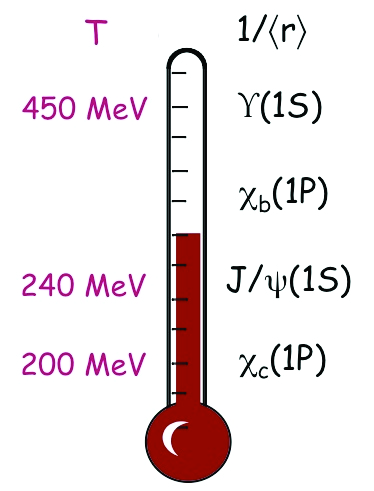
\includegraphics[width=0.3\linewidth]{Chapters/Analysis/Figs/QGP_thermometer.png}
\caption{Representation of a dissociation based QGP thermometer. The suppression of energetically ordered resonances can provide informations regarding the average kinetic energy of the formed QGP droplet.}
\label{fig:QGP_thermo}
\end{center}
\end{figure}

Is worth mentioning that, for bottomonium production, perturbative calculations of production rates in elementary nucleon-nucleon collisions are more reliable than for charmonium yields due to the higher mass of the bottom quark with respect to charm. 

In conclusion the study of bottomonium production can provide an independent measurement of QGP characteristics, adding up to charmonium measurements to better understand the dissociation and recombination contributions to quarkonia production.

\subsection{Complexity of bottomonium study}
Due to the higher mass of the constituting quarks, the abundance of bottomonium states in the final state of QGP evolution is much lower if compared to those of charmonium states.
This physical characteristic limits the available statistics.
In addition bottomonium production theoretical estimates \cite{Krouppa:2015yoa} indicate that its formation may occur before QGP thermalization \cite{Mauricio:2007vz}. 
In this situation, a quantitative description of the influence of the medium on the bound states becomes challenging.
Even if the dissociation temperatures may vary significantly between different models \cite{Brambilla:2010cs,Andronic:2015wma}, it is commonly accepted \cite{Burnier:2014ssa} that the spectral functions of the bottomonium states are affected by the high temperature of the surrounding medium.
This effect leads to much larger spectral widths than in vacuum.
Finally, even if the regeneration of bottomonium can be considered negligible at LHC energies, another production enhancement effect partly disrupts the possibility to use bottomonium states as a QGP thermometer. 
In fact, taking into account that feed-down processes from higher-mass resonances  are not negligible (around 40\% for the \upsis and 30\% for the \upsiss \cite{Andronic:2015wma}), the evaluation of the medium temperature via bottomonium measurements remains a complex endeavour.

\begin{figure}[!t]
\begin{center}
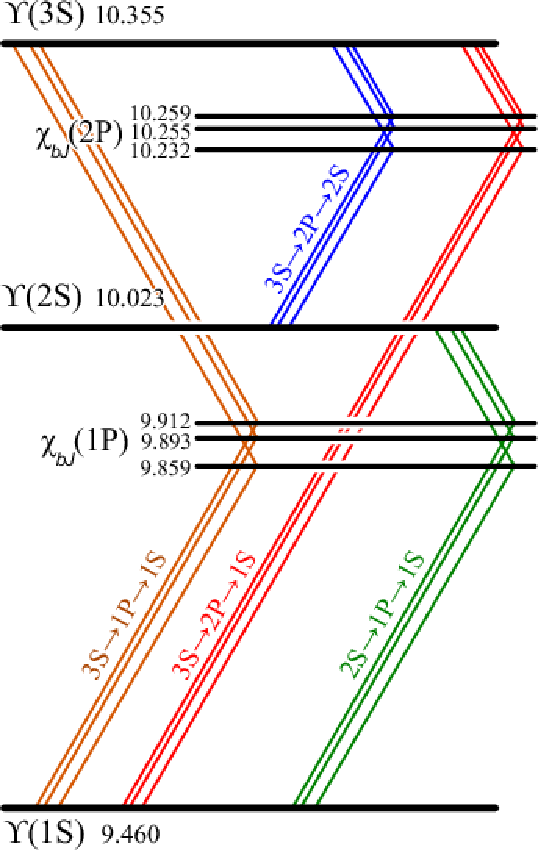
\includegraphics[width=0.45\linewidth]{Chapters/Analysis/Figs/BottomoniumSpectro.pdf}
\caption{Representation of possible feed-down patterns for bottomonium states as measured from BaBar collaboration and reported in \cite{Lees:2014qea}. The numbers refer to the masses as reported by the PDG. Each cascade terminates with the annihilation $\Upsilon(nS)\Rightarrow\mu^+\mu^-$, not shown. Splittings in the photon spectra for these cascades are due to the mass splittings in the intermediate states $\chi_{bJ}$ with J = 0, 1 or 2.}
\label{fig:BBSpectro}
\end{center}
\end{figure}

\subsection{Previous results}
Before the operations of LHC, the RHIC accelerator was leading the edge of QGP-oriented research.
The PHENIX collaboration measured the $J/\psi$ suppression in Au-Au collisions at $\sqrt{s_{_{\rm NN}}}=200$ GeV, highlighting a suppression strongly correlated with the centrality of the collision.
Given the much lower available energy at RHIC, with respect to the LHC, the recombination effects were not visible, yet unexpected.
The first $J/\psi$ measurements at the LHC disrupted the commonly accepted models, since, despite expectations, a much lower $J/\psi$ suppression was observed in the most central collisions at LHC at $\sqrt{s_{_{\rm NN}}}=2.76$ \rm{TeV} with respect to what had been observed at $\sqrt{s_{_{\rm NN}}}=200$ GeV at RHIC \ref{fig:LHC_RHIC_jpsi}.

\begin{figure}[!t]
\begin{center}
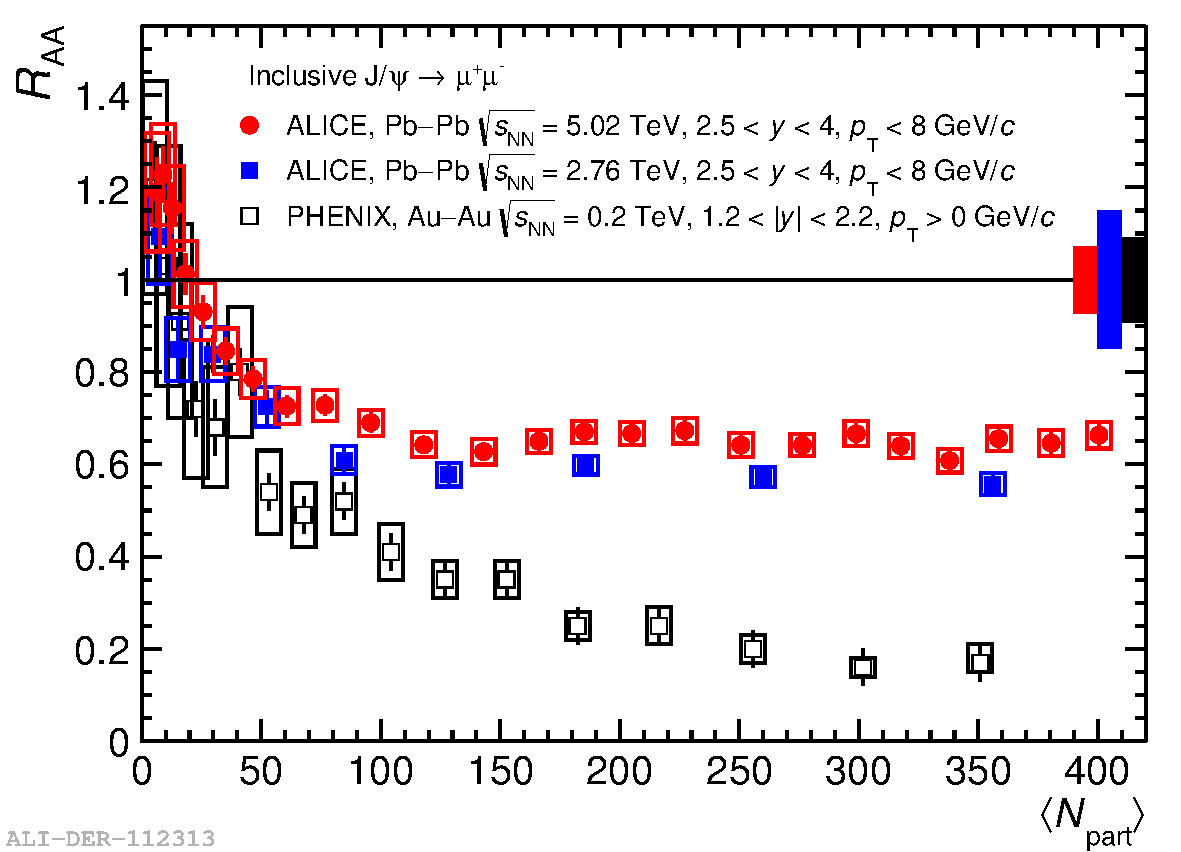
\includegraphics[width=0.8\linewidth]{Chapters/Analysis/Figs/2016-Sep-15-RAA_centr_Alice5_Alice276_Phenix.pdf}
\caption{$J/\psi$ nuclear modification factor measured by PHENIX (RHIC) at $\sqrt{s_{_{\rm NN}}}=200$ GeV (open black) and by ALICE at the LHC at $\sqrt{s_{_{\rm NN}}}=2.76$ and $5.02 \rm{TeV}$ (blue and red, respectively), as a function of the number of participant nucleons. The RHIC points appear systematically below ALICE ones over $<N_{part}>=50$, indicating a much lower suppression at LHC in the most central collisions. The two ALICE series appear to be in agreement over the whole centrality spectrum despite a factor ~$\times2$ for $\sqrt{s_{_{\rm NN}}}$. }
\label{fig:LHC_RHIC_jpsi}
\end{center}
\end{figure}

\begin{figure}[!t]
\begin{center}
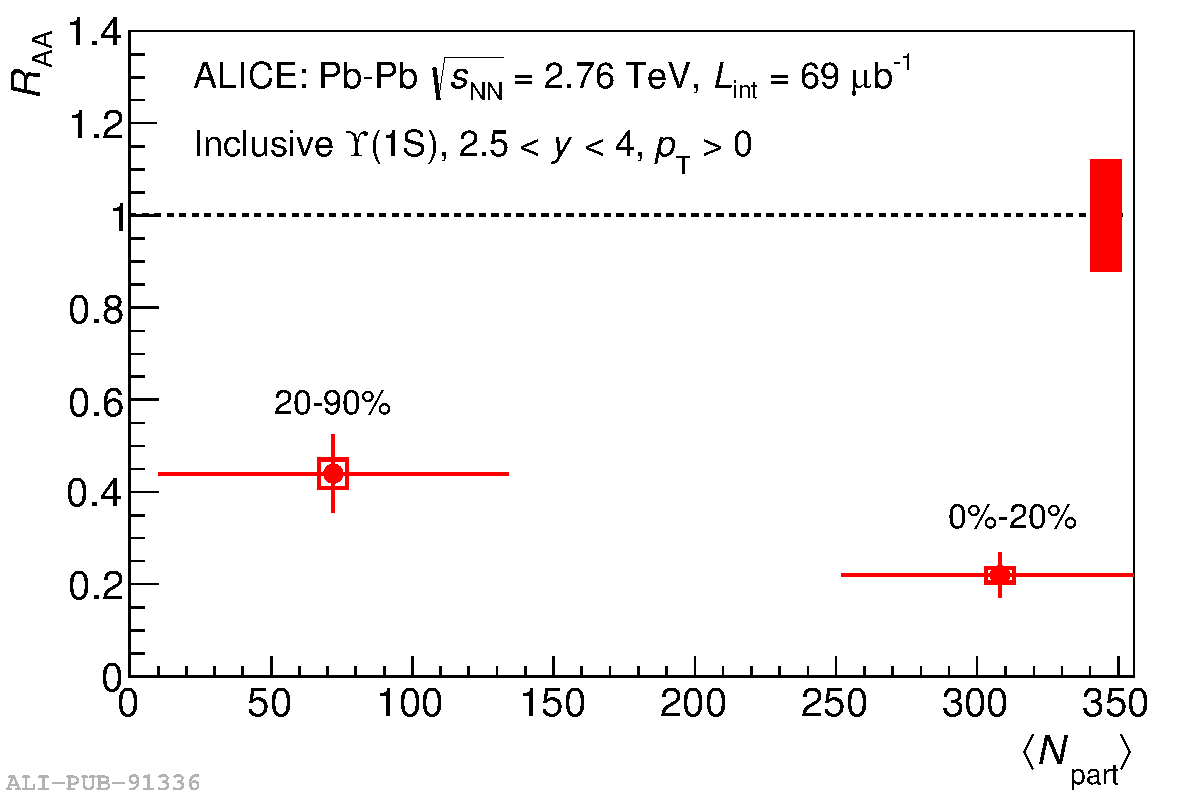
\includegraphics[width=0.8\linewidth]{Chapters/Analysis/Figs/2014-Dec-16-Raa_centr.pdf}
\caption{\upsi nuclear modification factor measured at the LHC by ALICE at $\sqrt{s_{_{\rm NN}}}=2.76$. Two centrality bins are shown, referring to the quoted centrality distribution percentiles.}
\label{fig:LHC_upsi}
\end{center}
\end{figure}

The theoretical models tuned to be able to describe the observed discrepancy included statistical regeneration mechanisms which were negligible at RHIC due to the much lower abundance of heavy quarks.
The provided models suggested that for \upsis production the regeneration effects would be still negligible, even at LHC collisions conditions, hence the bottomonium production studies were performed as well on the same data set.
As one can notice by performing a comparison between \ref{fig:LHC_RHIC_jpsi} and \ref{fig:LHC_upsi} the \upsi $R_{\rm{AA}}$ at $\sqrt{s_{_{\rm NN}}}=2.76$ appears to be similar to the $J/\psi$ one, measured at RHIC.
This observation is in agreement with the fact that the estimations of the total number of bottom quark pairs at the LHC and charm quark pairs at RHIC are almost aligned.
A strong suppression of the \upsis state in \pbpb collisions, with respect to properly scaled measurements from pp collisions, has been observed at $\sqrt{s_{_{\rm NN}}}=2.76$ \rm{TeV} by ALICE \cite{Abelev:2014nua} and CMS \cite{Chatrchyan:2012lxa,Khachatryan:2016xxp}, in the rapidity ranges $2.5<y<4$ and $|y|<2.4$, respectively \ref{fig:ALICE_CMS_upsi}. 

\begin{figure}[!t]
\begin{center}
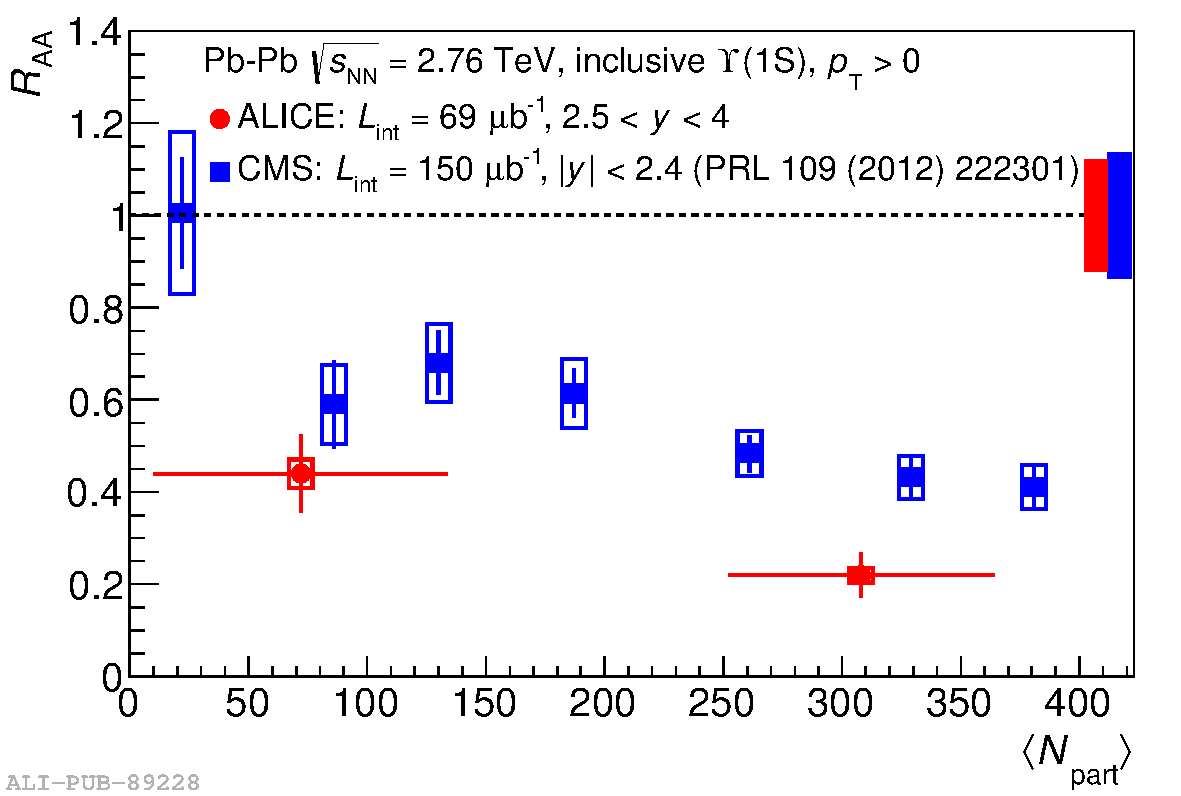
\includegraphics[width=0.47\linewidth]{Chapters/Analysis/Figs/2014-Nov-05-Raa_CMS_centr.pdf}
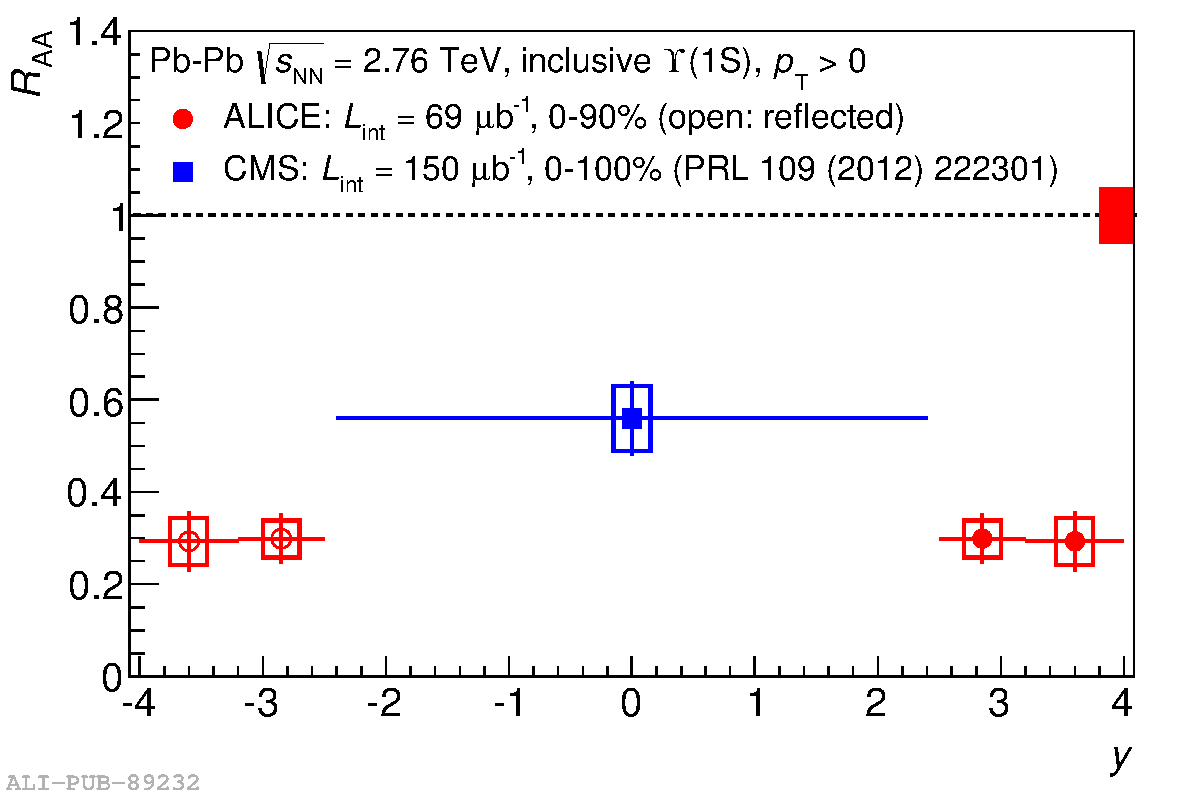
\includegraphics[width=0.47\linewidth]{Chapters/Analysis/Figs/2014-Nov-05-Raa_CMS_rap.pdf}
\caption{\upsis nuclear modification factor as a function of $<N_{part}>$ (left) and $y$ (right) measured by ALICE (red points, $2.5<y<4.0$) and CMS (blue points, $|y|<2.4$) at $\sqrt{s_{_{\rm NN}}}=2.76$ \rm{TeV}. A strong suppression is observed in both trends.}
\label{fig:ALICE_CMS_upsi}
\end{center}
\end{figure}

The suppression increases with the centrality of the collision, reaching about 60\% and 80\% for the most central collisions at mid-~\cite{Khachatryan:2016xxp} and forward rapidity~\cite{Abelev:2014nua}, respectively. 
Moreover, the \upsiss suppression reaches about 90\% and for \upsisss data are compatible with a complete suppression \cite{Khachatryan:2016xxp}. 
As a function of \pt the \upsis \raa, measured for $p_{\rm T}<20$ GeV/$c$ by CMS~\cite{Khachatryan:2016xxp}, is compatible with a constant value. 
When considering the $y$-dependence resulting from the comparison of ALICE and CMS results, there is an indication for a stronger suppression at forward $y$.
Transport models \cite{Zhou:2014kka,Du:2017qkv} fairly reproduce the experimental observations of CMS, while they tend to overestimate the $R_{\rm AA}$ values measured by ALICE. 
Similar conclusions can be obtained in the frame of an anisotropic hydrodynamic model \cite{Krouppa:2017jlg}. 
The comparison between $J/\psi$ and \upsis measurements performed by ALICE denotes a much stronger suppression for the former ($>3\sigma$) in the most central collisions \ref{fig:ALICE_jpsi_upsi}.

\begin{figure}[!t]
\begin{center}
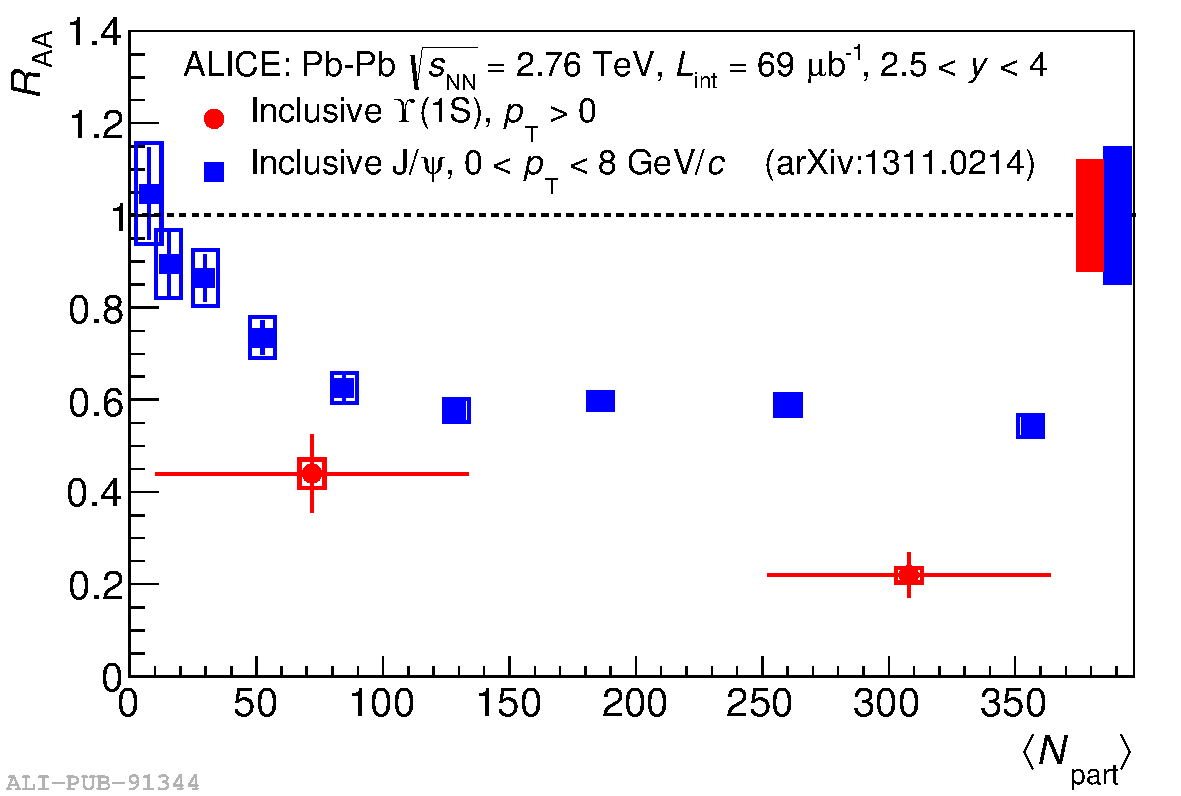
\includegraphics[width=0.8\linewidth]{Chapters/Analysis/Figs/2014-Dec-16-Raa_Jpsi_centr.pdf}
\caption{$J/\psi$ (blue) and \upsis (red) nuclear modification factor as a function of $<N_{part}>$ measured by ALICE at forward rapidity ($2.5<y<4.0$) at $\sqrt{s_{_{\rm NN}}}=2.76$ \rm{TeV}. The \upsis measurements are systematically and significantly below the $J/\psi$ points.}
\label{fig:ALICE_jpsi_upsi}
\end{center}
\end{figure}

The bottomonium suppression due to the QGP should be disentangled from the suppression due to Cold Nuclear Matter (CNM) effects, such as the nuclear modification of the parton distribution functions due to shadowing \cite{Eskola:1998df,Eskola:2009uj}, as well as parton energy loss \cite{Arleo:2012rs}.
These effects on the bottomonium production were studied in \ppb collisions by ALICE \cite{Abelev:2014oea} and LHCb \cite{Aaij:2014mza}, which reported for the \upsis a nuclear modification factor slightly lower than unity at forward rapidity and compatible with unity at backward rapidity, although with significant uncertainties \ref{fig:ALICE_pPb_jpsi_upsi}.
As a side note, in both rapidity ranges the compatibility between $J/\psi$ and \upsis is verified, suggesting a similar CNM effects contribution for charmonium and bottomonium.

\begin{figure}[!t]
\begin{center}
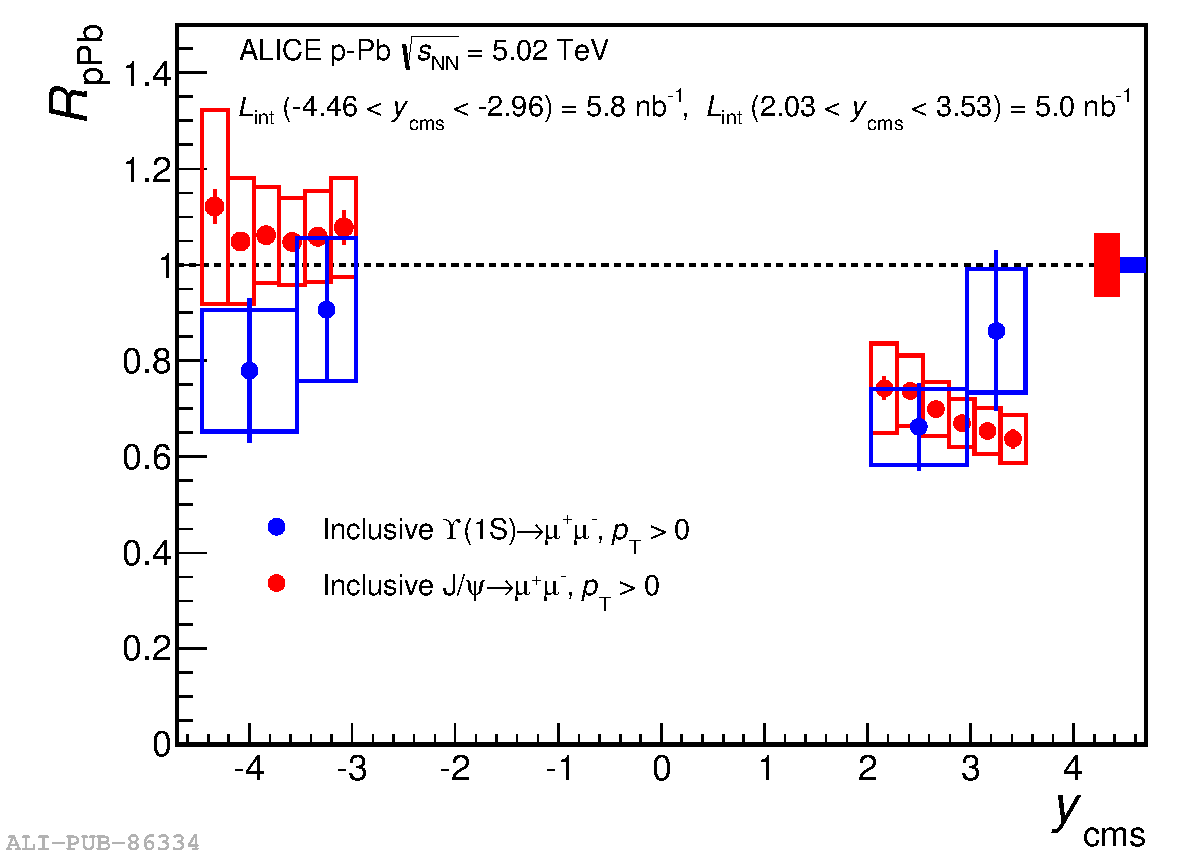
\includegraphics[width=0.8\linewidth]{Chapters/Analysis/Figs/2014-Oct-08-RpPb_Ups_Jpsi_b.pdf}
\caption{$J/\psi$ (red) and \upsis (blue) nuclear modification factor as a function of $y$ measured by ALICE is p-Pb collisions ($-4.46<y<-2.96$ and $2.03<y<3.53$) at $\sqrt{s_{_{\rm NN}}}=5.02$ \rm{TeV}. The \upsis measurements compatible with unity at backward rapidity and show partial suppression at forward rapidity. In both cases the \upsis measurements are compatible with $J/\psi$ ones.}
\label{fig:ALICE_pPb_jpsi_upsi}
\end{center}
\end{figure}

$p-Pb$ collisions are the CNM baseline since the achieved energy density is not enough to cause QGP production, but the nucleons of the colliding nuclei might be perturbed by the others.
Recently, ATLAS results indicate a significant suppression of the \upsis around mid-rapidity~\cite{Aaboud:2017cif}.  
Additional measurements at forward/backward rapidity with higher statistics, are needed to fully constrain the models and perform a meaningful extrapolation of CNM effects to \pbpb collisions.

\section{The Large Hadron Collider}
The Large Hadron Collider (LHC) is the most powerful particle accelerator ever built.
It is the largest element of the CERN acceleration facility and has been placed in the same $27km$ long tunnel previously used for the Large Electron Positron collider (LEP) placed between $45$ and $170m$ underground \ref{fig:accelerators}.
Some of the previous CERN accelerators are connected together and now used as pre acceleration steps for the final LHC injection.

\begin{figure}[!t]
\begin{center}
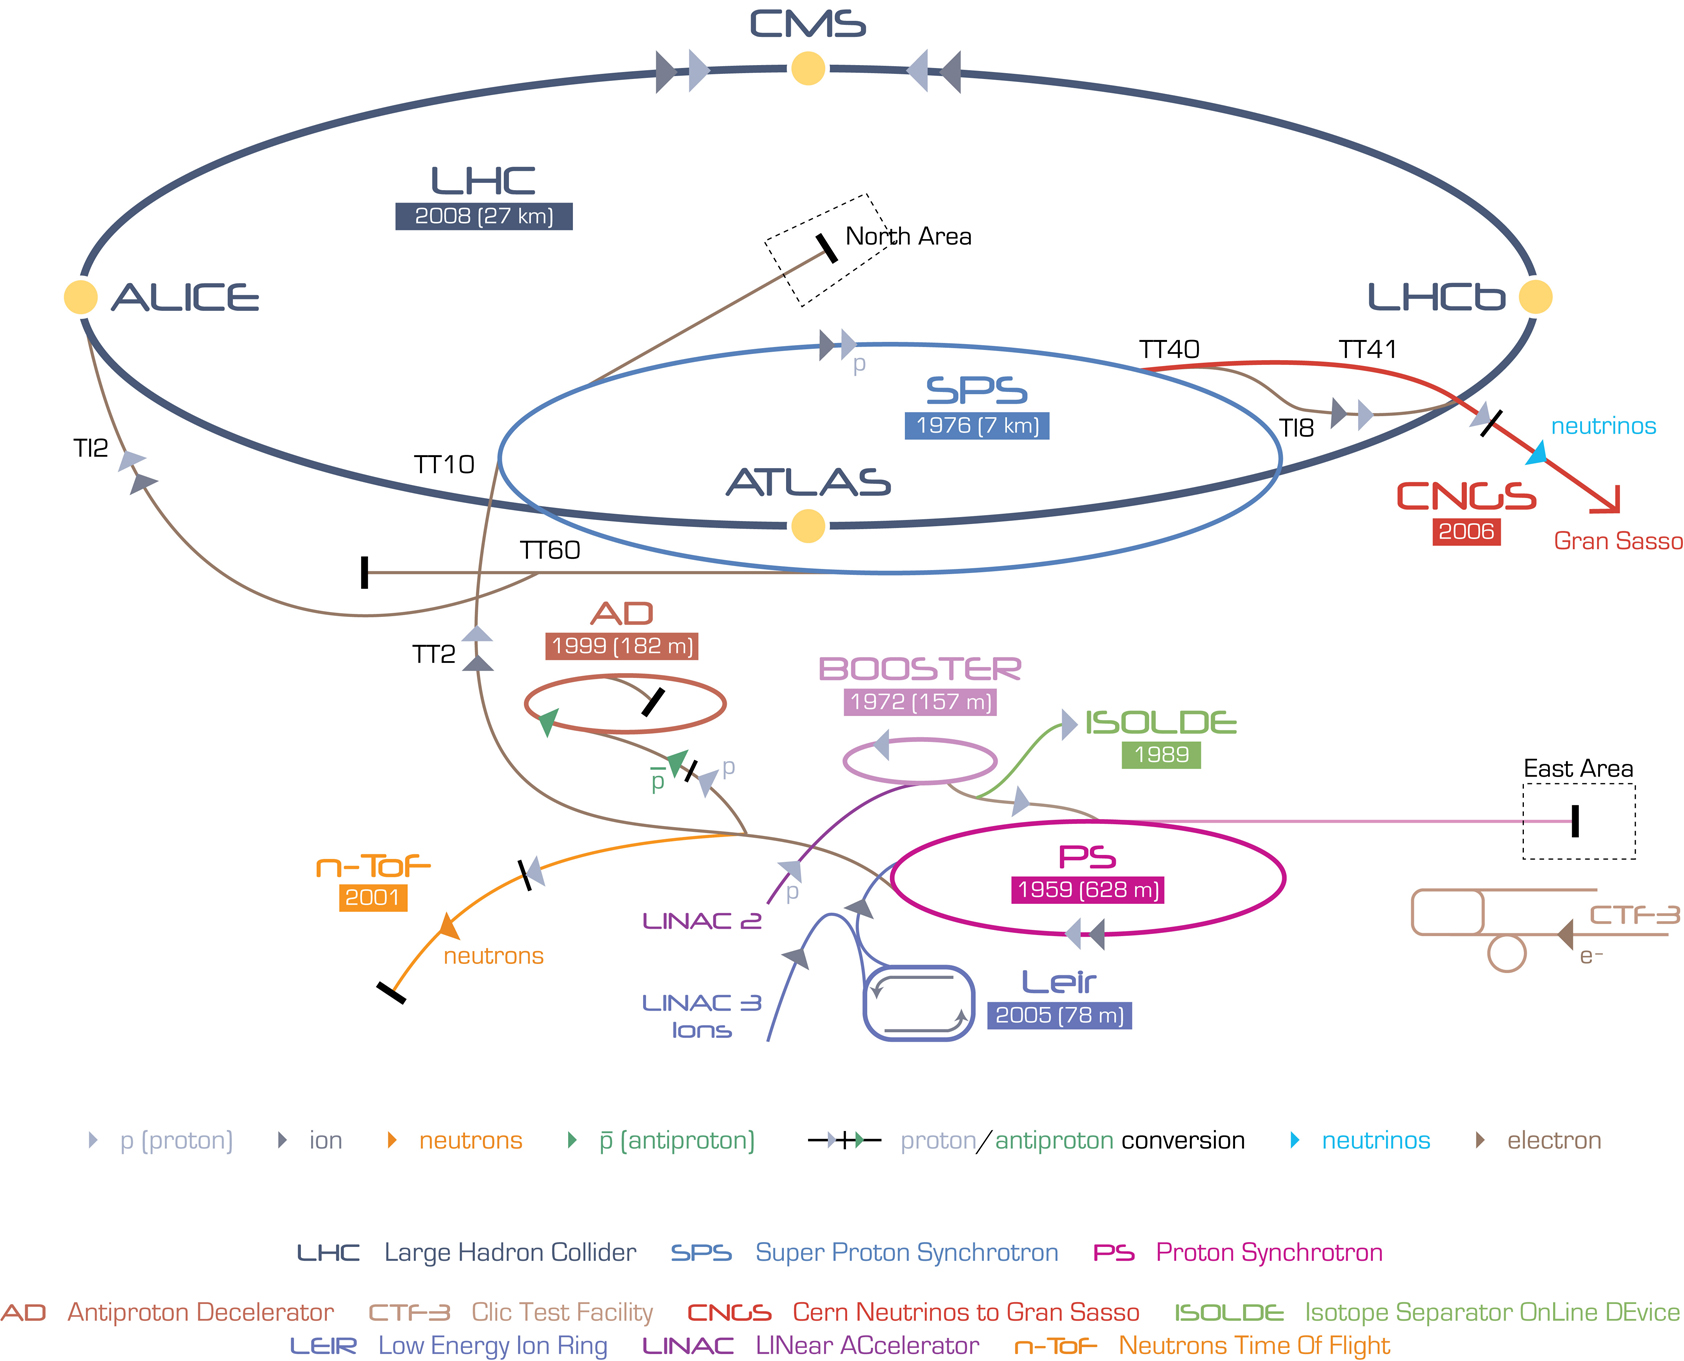
\includegraphics[width=\linewidth]{Chapters/Introduction/Figs/Cern-Accelerator-Complex.jpg}
\caption{Schematic representation of the CERN accelerator complex.}
\label{fig:accelerators}
\end{center}
\end{figure}

The LHC allows one to perform proton-proton, proton-Pb and Pb-Pb collisions (and lately also Xe-Xe).
For what concerns the pre-acceleration of protons the CERN LInear ACcelerators (LINAC), the Proton Synchrotron Booster (PSB), the Proton Synchrotron (PS) and the Super Proton Synchrotron are used upstream the LHC.
The heavy nuclei are instead firstly produced, ionized and accelerated in the Low Energy Ion Ring (LEIR) and then injected directly in the PS-SPS chain.
Thanks to the superconducting magnets (dipoles, quadrupoles and higher order ones) protons and nuclei can be accelerated up to $14TeV$ and $5.5TeV$ respectively.
Along the LHC ring four main experiments are placed: ALICE (A Large Ion Collider Experiment), CMS (Compact Muon Solenoid), ATLAS (A Toroidal LHC ApparatuS) and LHCb (Large Hadron Collider beauty).

%********************************** %Third Section  *************************************
\section{ALICE experimental setup} %Section - 1.3
The main purpose of the ALICE experiment is the study of the physics of strongly interacting matter in ultra-relativistic heavy-ion collisions. It is also designed for proton-proton and proton-nucleus collisions which represent an important part of its physics program. The experiment itself can be divided into three main sectors:
\begin{itemize}
    \item global detectors are used for triggering, event characterization and beam luminosity measurements;
    \item central barrel detectors are embedded into a solenoid with a magnetic field of B = 0.5 T and are used for tracking and identification of charged particles and photons;
    \item muon spectrometer covers the forward region with respect to the interaction point and its detectors are designed for muon tracking and trigger.
\end{itemize}

\begin{figure}[!t]
\begin{center}
\includegraphics[width=\linewidth]{Chapters/Introduction/Figs/ALICE-Setup.jpg}
\caption{Schematic of ALICE detectors setup, with a maximised view of the innermost detectors.}
\label{fig:ALICEsetup}
\end{center}
\end{figure}

The detector is completed by an array of scintillators to trigger on cosmic rays.
A more detailed discussion of the ALICE detectors is reported in the following sections.

\subsection{Central barrel}
The mid rapidity section of the ALICE experimental apparatus is named central barrel.
It includes many detectors, each of them with different purposes.
The structure surrounds the interaction point, covering the pseudorapidity range $|\eta| < 0.9$, and it is inside the $0.5 T$ magnetic field generated by a warm solenoidal magnet originally employed by the L3 collaboration.

\subsubsection{Inner Tracking System (ITS)}
The ITS is the closest detector to the beam pipe of the ALICE apparatus.
Its purposes are the identification of primary collision vertexes, the reconstruction of secondary vertexes from heavy particles decays and the tracking and identification of low momentum particles.
The spatial resolution of the ITS is lower than $100\mu~m$.
It is completely made of silicon detectors, implemented using three technologies.
Six layers compose the ITS:
\begin{itemize}
    \item Silicon Pixel Detector (SPD): two layers located at 3.9 and 7.6 cm from the interaction point, they are important for a high spatial resolution and for their very fast response;
    \item Silicon Drift Detector (SDD) : two layers located at 15 and 23.9 cm from the interaction point, they provide a bi-dimensional spatial information with a lower resolution than SPD;
    \item Silicon Strip Detector (SSD) : two layers located at 38 and 43 cm from the interaction point, they provide a complementary information on track positions.
\end{itemize}


\begin{figure}[!h]
\begin{center}
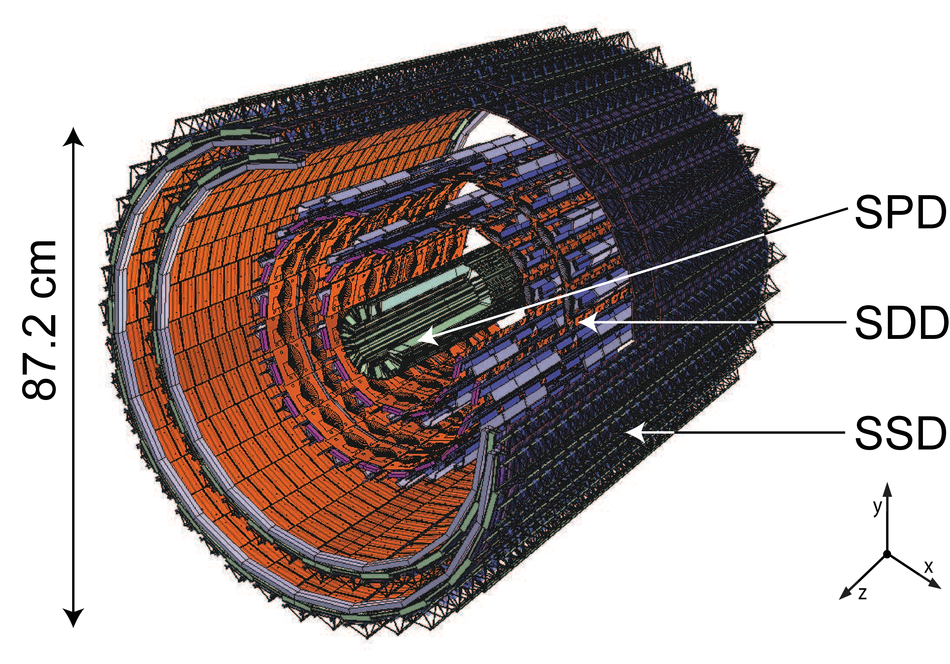
\includegraphics[width=0.7\linewidth]{Chapters/Introduction/Figs/its.png}
\caption{Schematic of the ALICE ITS.}
\label{fig:ITS}
\end{center}
\end{figure}

\subsubsection{Time Projection Chamber (TPC)}
The Time Projection Chamber is the main tracking detector of the central barrel.
It is a $88 m^3$ cylindrical detector filled with a gas mixture of $Ar$−$CO_2$ $(90-10\%)$.
Its volume is limited by two end-plates acting as segmented read-out electrodes. 
In addition an electrode is placed in the middle of the TPC, dividing it into two halves.
The ionizing particles crossing the detectors ionize the gaseous mixture.
The freed electrons drift towards the read-out electrodes.
As a result the side projection of the track is obtained directly from the electrodes, while the third coordinate of the points is obtained through the time of arrival of each segment.

\begin{figure}[!h]
\begin{center}

\includegraphics[width=0.7\linewidth]{Chapters/Introduction/Figs/tpc.png}
\caption{Representation of the TPC with some details of the layout.}
\label{fig:TPC}
\end{center}
\end{figure}

\subsubsection{Transition Radiation Detector (TRD)}
The Transition Radiation Detector is the main electron detector in ALICE.
It consists of six layers of multi-wire proportional chambers, filled with a mixture of $Xe$ and $CO_2$, equipped with a radiator made of optical fiber embedded in plastic foam directly glued on the electrode.
It is designed to provide charged-particle tracking, electron identification via transition radiation and pion rejection. 
The combination of ITS, TPC and TRD information provides a momentum resolution in the central barrel good enough to measure high pt tracks down to $100 GeV/c$ and a mass resolution about $100 MeV/c$.

\begin{figure}[!h]
\begin{center}
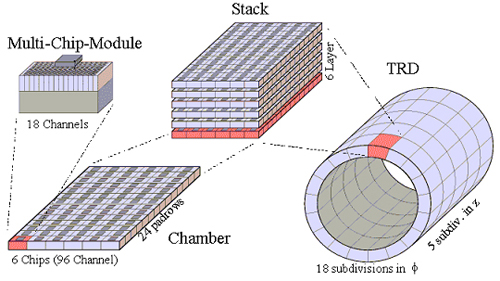
\includegraphics[width=0.7\linewidth]{Chapters/Introduction/Figs/trd.jpg}
\caption{Schematic of the ALICE TRD with an highlight on the modular struture of the detector.}
\label{fig:TRD}
\end{center}
\end{figure}

\subsubsection{Time Of Flight (TOF)}
The Time Of Flight detector is designed to identify charged particles with a momentum from $1 GeV/c$ to few $GeV/c$, extending the TPC particle identification capabilities. 
It is composed by multi-gap resistive plate chambers arranged into $18$ sectors in a cylindrical shell placed $3.7 m$ far from the beam pipe. 
The TOF provides the arrival time of a particle in the detector’s volume with a resolution of $80 ps$, completing the information gathered by TPC and TRD, in terms of identification of the detected particles, in particular separating $\pi/K$ up to $2.2 GeV/c$ and $K/p$ up to $4 GeV/c$.

\begin{figure}[!h]
\begin{center}
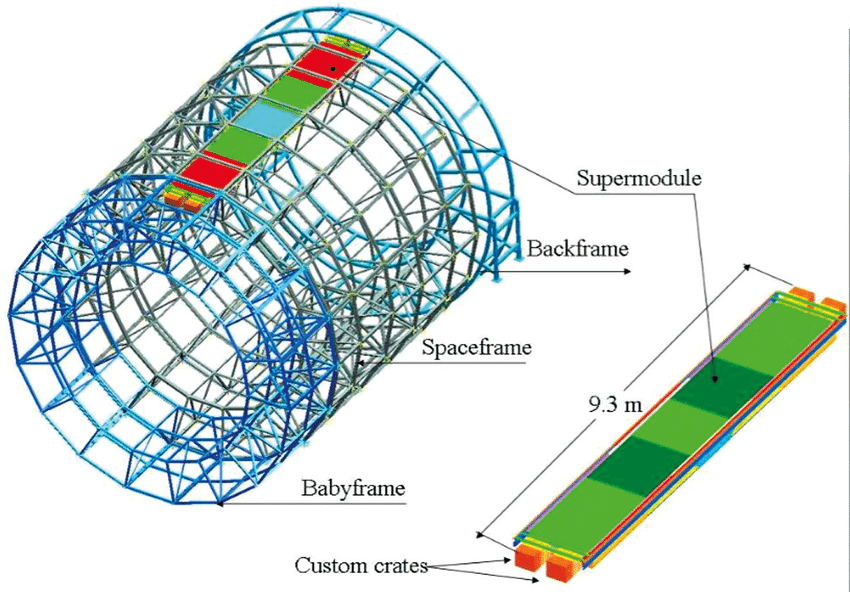
\includegraphics[width=0.7\linewidth]{Chapters/Introduction/Figs/tof.png}
\caption{Schematic of the ALICE TOF. A detector module is represented along with the support structure.}
\label{fig:TOF}
\end{center}
\end{figure}

\subsubsection{High Momentum Particle Identification Detector (HMPID)}
The main purpose of HMPID is to enhance the particle identification capability beyond the range allowed by ITS, TPC and TOF. 
It is based on proximity focusing Ring Imaging Cherenkov (RICH) counters and consists of seven modules mounted in an independent support cradle. 
When a fast charged particle traverses the $15 mm$ layer of liquid $C_6F_{14}$, Cherenkov photons are emitted and detected by the photon counter, which is a thin layer of $CsI$ deposited onto the pad cathode of multi-wire proportional chambers.

\begin{figure}[!h]
\begin{center}
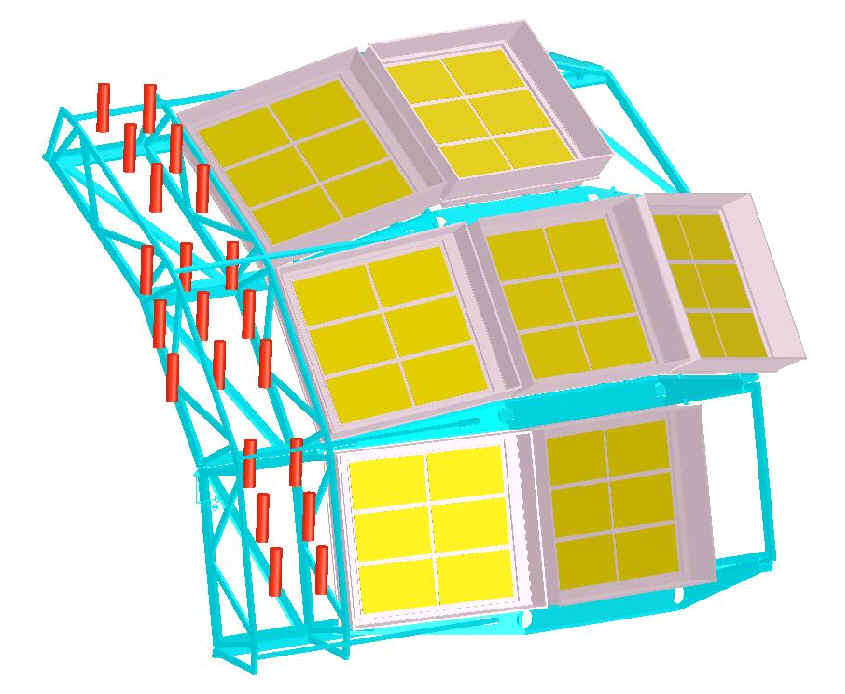
\includegraphics[width=0.4\linewidth]{Chapters/Introduction/Figs/hmpid.jpg}
\caption{The HMPID layout.}
\label{fig:HMPID}
\end{center}
\end{figure}

\subsubsection{PHOton Spectrometer (PHOS)}
The Photon Spectrometer is a high resolution electromagnetic spectrometer which consists of a highly segmented electromagnetic calorimeter of lead-tungstate crystals.
It is located on the bottom of the ALICE experimental apparatus, covering the pseudorapidity range $|\eta| < 0.12$, and it is designed for measuring photons and neutral mesons ($\pi_0$ and $\eta$) through their decays into two photons up to momenta about $10 GeV/c$.

\begin{figure}[!h]
\begin{center}
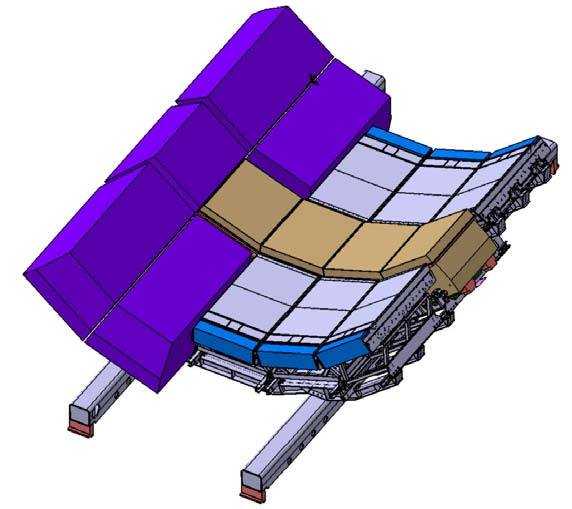
\includegraphics[width=0.5\linewidth]{Chapters/Introduction/Figs/phos.jpg}
\caption{The PHOS layout.}
\label{fig:PHOS}
\end{center}
\end{figure}

\subsubsection{ElectroMagnetic Calorimeter (EMCal)}
Positioned on the top of the ALICE structure, close to the solenoid coils, EMCal is designed to study jet quenching and it is used for triggering on photons, electrons and jets.
It is composed by 1152 towers of lead scintillators wiht photomultiplier readout and it covers a pseudo-rapidity range of $|\eta| < 0.7$.

\begin{figure}[!h]
\begin{center}
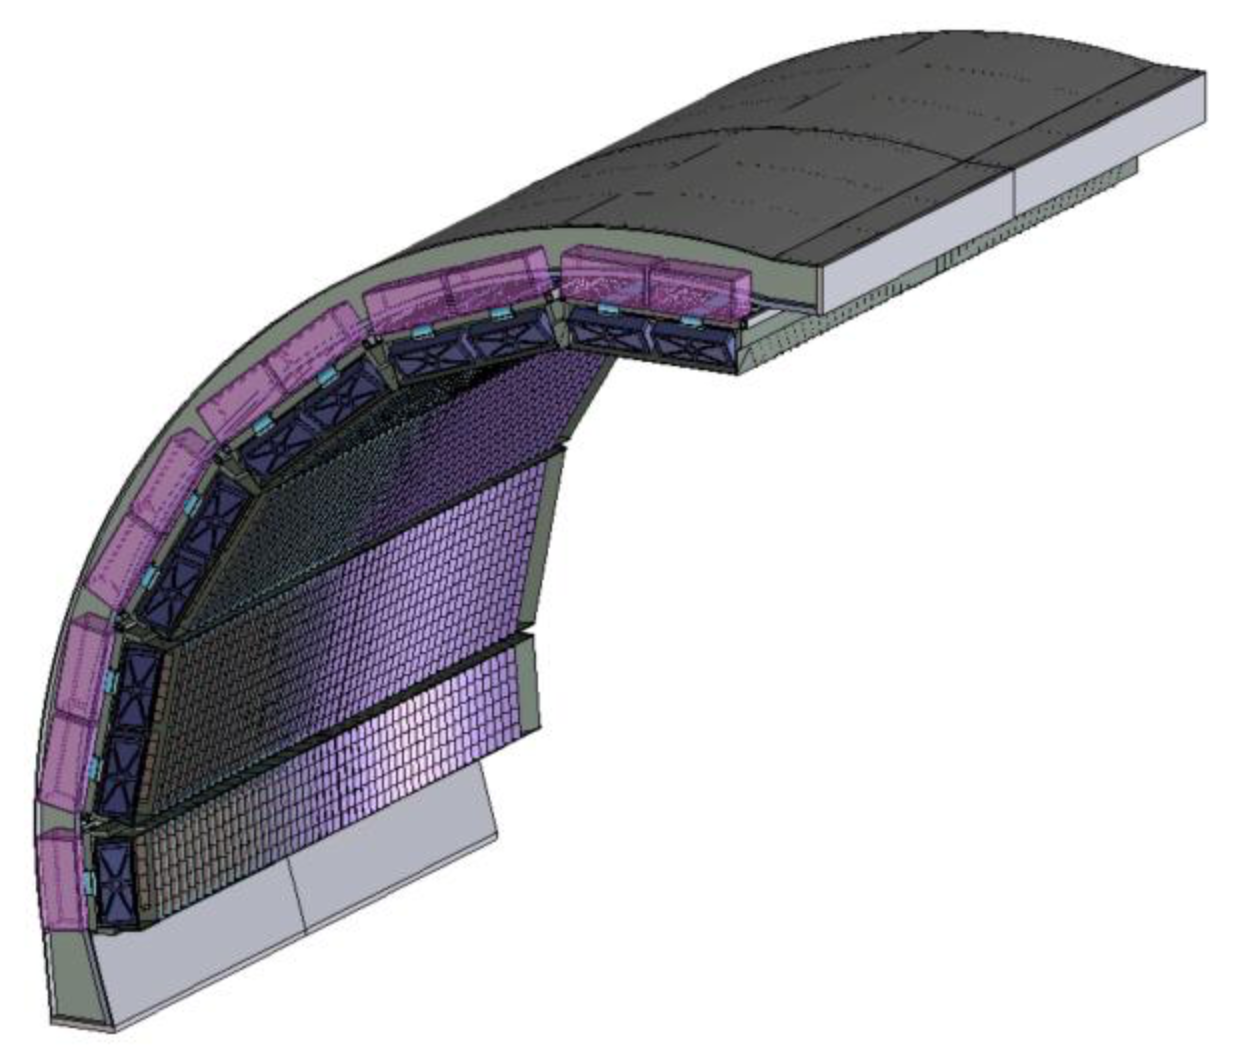
\includegraphics[width=0.5\linewidth]{Chapters/Introduction/Figs/emcal.png}
\caption{The EMCal layout.}
\label{fig:EMCAL}
\end{center}
\end{figure}

\subsection{Muon spectrometer}
The Muon Spectrometer is designed to measure muon production from the decays of quarkonia ($J/\psi$ , $\psi(2S)$ , $\Upsilon(1S)$, $\Upsilon(2S)$ and $\Upsilon(3S)$), low mass vector mesons ($\rho$, $\omega$ and $\phi$), heavy flavor hadrons and $W^\pm$ and $Z^0$ bosons. 
The detector is located in the pseudorapidity region $−4.0 < \eta < −2.5$ and it has a total length of $17 m$. 
It is composed by a system of passive absorbers, a dipole magnet, a muon tracker, an iron wall and a muon trigger system. 
The main components of the Muon Spectrometer will be discussed with more details in the following.

\begin{figure}[!h]
\begin{center}
\includegraphics[width=\linewidth]{Chapters/Introduction/Figs/spectro.png}
\caption{Schematic representation of ALICE with highlighted muon spectrometer components.}
\label{fig:spectro}
\end{center}
\end{figure}

\subsubsection{Absorbers system}
The Muon Spectrometer requires some shielding to reduce the otherwise large background produced expecially in nucleus-nucleus collisions.
For this reason it is equipped with a system of absorbers:
\begin{itemize}
    \item front absorber: this absorber is located inside the central barrel as close as $90 cm$ from the interaction point. The purpose of the front absorber is to filter out hadrons and to reduce the background generated by pions and kaons decays. The materials the front absorber is made of have been chosen to limit the multiple scattering of muons and leptons in general. The section of the front absorber placed closest to the interaction point is made of carbon to limit multiple scattering thanks to the low Z. The next sections of the absorber are composed of concrete to absorb secondary particles and low energy protons and neutrons. The whole absorber is coated of lead and boronated polyethilene to avoid decay products recoils in the TPC;
    \item beam shield: the beam pipe is layered with this shielding made of tungsten, lead and stainless steel to shield the muon spectrometer from the particles produced in the interactions between low angle particles and gas residuals inside the beam pipe;
    \item iron wall: this $1.2m$ thick absorber is placed between two detector systems and acts as a filter capable of absorbing everything but muons and other penetrating particles;
    \item rear absorber: an additional passive element has been installed around the connection hole between the experiment cave with the LHC tunnel in order to further remove products of gas interaction.
\end{itemize}

\subsubsection{Dipole magnet}
Located at $7m$ from the interaction point, the dipole magnet is used to determine the momentum and the electric charge of particles produced in the interaction point.
The value of the magnetic field provided (the magnetic flux density is $0.7T$ and the integrated value is $3T\cdot~m$) is defined by requirements of mass resolution.
The magnetic field is perpendicular to the beam pipe.
The definition of bending and non-bending planes follows the magnetic field direction.
The plane $zy$ is defined as the bending plane, since the dipole action deviates muons in this direction, and the plane $xz$ as the non-bending plane.

\begin{figure}[th]
\begin{center}
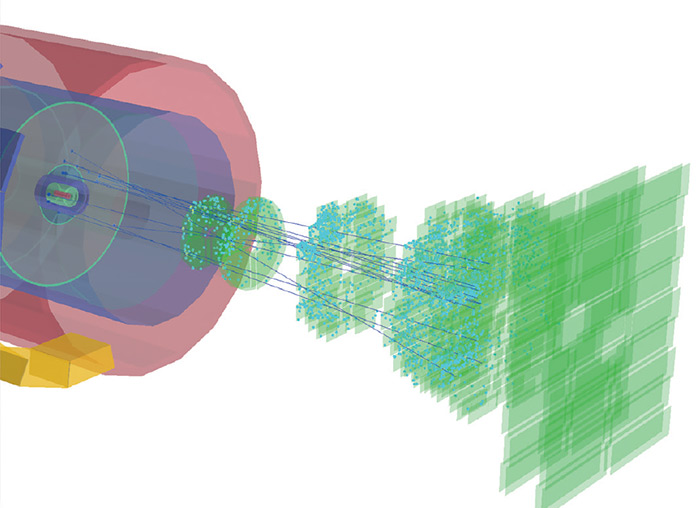
\includegraphics[width=\linewidth]{Chapters/Introduction/Figs/muon_mtr_mch.jpg}
\caption{Digital representation of the layout of the muon chambers and muon trigger system, shown in green.}
\label{fig:mch_mtr}
\end{center}
\end{figure}

\subsubsection{Muon Tracker or Muon Chambers (MCH)}
The tracking system is made of $10$ multi wire proportional chambers arranged in $5$ stations of $2$ chambers each.
The anode is implemented as wires placed between the readout sides, while the readout electrodes are strips or pads placed on the sides.
The produced electrons generate an avalanche drifting towards the nearest anode wire, and the resulting ion cloud induces a charge distribution on the cathode planes, allowing to determine the position of the track.
The size of the chambers depends on the spectrometer’s angular coverage, considering the deviation of muons by the magnetic field (because for this reason stations from 3 to 5 have larger dimensions).
The pad size of all the chambers is smaller close to the beam pipe, in order to take into account the higher density of particles produced in that region.
The spatial resolution is better than $2 mm$ and all the chambers are made of composite material ($< 3\%$ $X_0$ per chamber) to minimize the scattering of the muons in order to obtain the required resolution. 
To limit the occupation rate to a maximum of $5\%$ the full set of chambers has more than $1$ million channels.

\subsubsection{Muon Trigger (MTR)}
The muon trigger system is designed to tag high $p_T$ muons produced in heavy quarkonia and open heavy flavour mesons decays.
Thank to a configurable $p_T$ threshold, the system is able to provide trigger signals to select interesting events and to discard events with only low $p_T$ muons, which mainly come from pions and kaons decays.
The muon trigger system is composed of 72 Resistive Plate Chambers with $x-y$ read out, organized in $4$ planes paired in two stations to provide redundancy.
Each RPC consists of two planes, made of bakelite and separated by 2 mm of gas.
A charged particle passing through the gas ionizes it, causing the formation of an avalanche of secondary electrons, which are picked up by the copper strips placed outside the chambers.
The pattern of hit strips, gathered by the front-end electronics, is sent to the local trigger board which provides a first measure of muon momentum and gives the trigger decision.
The latter is performed considering the deviation of a track with respect to the track with infinite momentum ($p_T \rightarrow \infty$). The deviation has to be smaller than a certain value, which corresponds to the $p_T$ cut.
%!TEX root = ../thesis.tex
%*******************************************************************************
%*********************************** First Chapter *****************************
%*******************************************************************************

\chapter{Monitoring of the MTR detector}  %Title of the First Chapter

% \ifpdf
%     \graphicspath{{Introduction/Figs/Raster/}{Introduction/Figs/PDF/}{Introduction/Figs/}}
% \else
%     \graphicspath{{Introduction/Figs/Vector/}{Introduction/Figs/}}
% \fi


%********************************** %First Section  **************************************
\section{The ALICE DCS system} %Section - 2.1 

% \nomenclature[z-cif]{$CIF$}{Cauchy's Integral Formula}                                % first letter Z is for Acronyms 
% \nomenclature[a-F]{$F$}{complex function}                                                   % first letter A is for Roman symbols
% \nomenclature[g-p]{$\pi$}{ $\simeq 3.14\ldots$}                                             % first letter G is for Greek Symbols
% \nomenclature[g-i]{$\iota$}{unit imaginary number $\sqrt{-1}$}                      % first letter G is for Greek Symbols
% \nomenclature[g-g]{$\gamma$}{a simply closed curve on a complex plane}  % first letter G is for Greek Symbols
% \nomenclature[x-i]{$\oint_\gamma$}{integration around a curve $\gamma$} % first letter X is for Other Symbols
% \nomenclature[r-j]{$j$}{superscript index}                                                       % first letter R is for superscripts
% \nomenclature[s-0]{$0$}{subscript index}                                                        % first letter S is for subscripts
%!TEX root = ../thesis.tex
%*******************************************************************************
%*********************************** First Chapter *****************************
%*******************************************************************************

\chapter{Study of bottomonium production in Pb-Pb collisions at$\ $ \texorpdfstring{$\sqrt[]{s_{NN}}=5.02 \rm{TeV}$}{sqrt(Snn)=5.02\ \rm{TeV}}}

%********************************** %First Section  **************************************
\section{Operational definition of nuclear modification factor}
In order to study the modification of \upsi production in Pb-Pb collisions at $\sqrt{s_{_{\rm NN}}}=5.02$~\rm{TeV} the evaluation of $R_{\rm AA}$ should be performed through an expression based on the one presented in \ref{intro_glauber}:
\begin{equation} \label{eqn:raa}
R_{\rm{AA}} = \frac{N^{\Upsilon}}{ {\rm BR}_{\Upsilon \rightarrow \mu^{+} \mu^{-}} \cdot  (A\times\epsilon)_{\Upsilon \rightarrow \mu^{+} \mu^{-}} \cdot  N_{MB} \cdot \sigma_{\rm pp}^{\Upsilon} \cdot \langle T_{\rm AA} \rangle } ~~
\end{equation}
where:
\begin{itemize}
\item $N^{\Upsilon}$ is the number of detected resonance decays to muon pairs, while ${\rm BR}_{\Upsilon \rightarrow \mu^{+} \mu^{-}}$ is the branching ratio for the dimuon decay \cite{Agashe:2014kda};
\item The $(A\times\epsilon)_{\Upsilon \rightarrow \mu^{+} \mu^{-}}$ factor is the product of acceptance and detection efficiency, specific for the $\Upsilon$ state under study;
\item $N_{\text{MB}}$ is the equivalent number of minimum bias events used for the analysis and is defined as $N_{\mu \mu-MB} * F_{norm}$, where $F_{norm}$ is the inverse probability of having an unlike-sign dimuon triggered sample in a MB event \cite{Adam:2016rdg};
\item $\sigma_{\rm pp}^{\Upsilon}$ is the reference \pp cross section and $\langle T_{\rm AA} \rangle$ represents the nuclear overlap function, which is evaluated in different centrality classes using the Glauber model~\cite{Abelev:2013qoq,Adam:2015ptt}.
\end{itemize}

%%%%%%%%%%%%%%%%%%%%%%%%%%%%%%%%%%%%%%%%%%%%%%%%
\section{Experimental apparatus and data sample}

An extensive description of the ALICE apparatus can be found in section \ref{ALICE_apparatus}.
This analysis is based on muons detected at forward rapidity ($2.5<y<4.0$) with a combination of detectors from the central barrel and the muon spectrometer~\cite{Aamodt:2011gj}. 

In this analysis the reconstruction of the primary vertex has been performed using the Silicon Pixel Detector \cite{Aamodt:2010aa}.

The Minimum Bias (MB) trigger is provided by the logical AND of the signals from the two scintillating array tiles of the V0 detector \cite{Abbas:2013taa} and the signal in the beam counters.

The MB trigger is fully efficient for the studied 0--90\% most central collisions.
The V0 detector provides the centrality estimate through a Glauber model fit of the signal amplitudes \cite{Abelev:2013qoq,Adam:2015ptt}.

The Zero Degree Calorimeters (ZDC), given their capability of detection of spectator protons, neutrons and nuclear fragments, allowed for the rejection of events corresponding to an electromagnetic interaction of the colliding Pb nuclei \cite{ALICE:2012aa}.

The muon spectrometer covers the pseudorapidity range $-4<\eta<-2.5$.
The muon tracker and the muon trigger are the detectors devoted to the reconstruction and identification of the produced muons, respectively.
The trigger condition used for data taking is a dimuon trigger.
% Given the extension of the muon spectrometer through a dipole magnet, the discrimination of muons charge sign can be achieved via the evaluation of their bending direction.
Thanks to the muon spectrometer geometry and to the presence of a dipole magnet, the electric charge sign of muons can be established at the trigger level, looking at the tracks bending direction.
Further details are given in section \ref{ALICE_spectrometer} of this thesis.
% The adopted trigger is then formed by the logical AND of the MB trigger and the presence in the muon trigger of a pair of muons with opposite charge sign, each with a pt larger than about 1 GeV/c.
The adopted trigger is then formed by the logical AND of the MB trigger and the presence in the muon trigger of a pair of muons with opposite charge sign, each with a pt larger than about $1\ GeV/c$ ($\mu \mu-MB$ trigger). 
% The number of equivalent Minimum Bias events can be then obtained as $N_{\mu \mu-MB} * F_{norm}$, where $N_{\mu \mu-MB}$ is the number of analyzed dimuon triggers and $F_{norm}$ is the inverse of the probability to have an unlike-sign dimuon triggered sample in a MB event \cite{Adam:2016rdg}.

% The former is provided by V0, the latter by the muon trigger.
In addition, in order to perform the event mixing procedure by artificially combining uncorrelated unlike-sign muons into dimuons for background reduction, the single muon trigger has been recorded.

The data used for this analysis has been collected between October and November 2015, during the first \pbpb data taking campaign of the  LHC RUN2.
A total of 137 runs belonging to this period has been analyzed.
In the present analysis the data sample corresponds to an integrated luminosity $L_{\rm int}\approx 225$ $\mu$b$^{-1}$ in the centrality interval 0--90\%, that has been divided into four centrality classes: 0--10\%, 10--30\%, 30--50\% and 50--90\%.

% %%%%%%%%%%%%%%%%%%%%%%%%%%%%%%%%%%%%%%%%%%%%%%%%
\section{Signal extraction}

\begin{figure}[!b]
\begin{center}
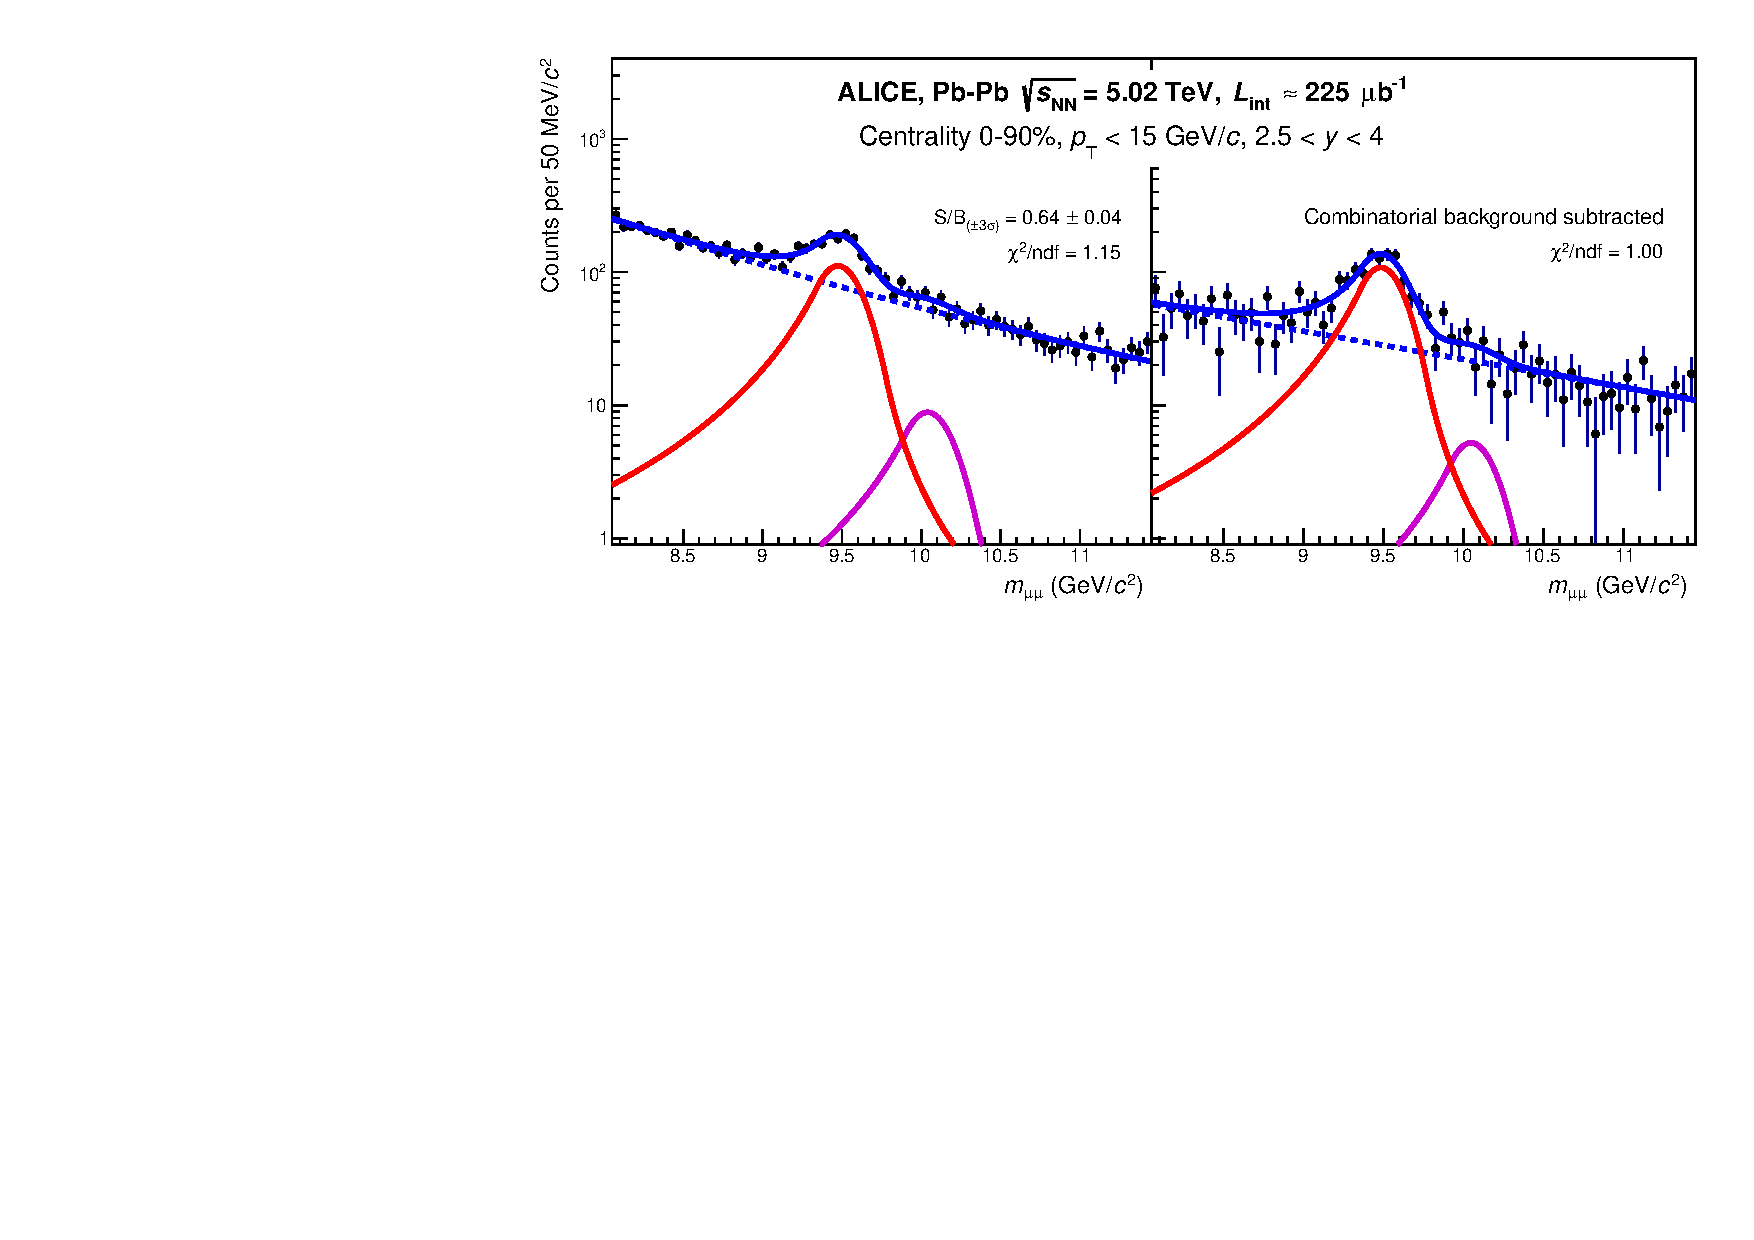
\includegraphics[width=0.8\linewidth]{Chapters/Analysis/Figs/InvMass_Upsilon_Performance_Ylog.pdf}
\caption{Dimuon invariant mass distribution (left) and combinatorial background subtracted distribution (right) in the mass region of bottomonium signals. Solid (dotted) lines correspond to signal (background) functions. The sum of the various functions is also shown as a solid line.}
\label{fig:mass_dist}
\end{center}
\end{figure}

% The analysis subject of this thesis has been performed looking at the \upsi production in the dimuon decay channel at forward rapidity.
The signal yields are evaluated by performing fits to the $\mu^+\mu^-$ invariant mass distributions.
In order to improve the purity of the dimuon sample a set of selection criteria has been applied to the muon tracks:
\begin{itemize}
\item Each track must have a transverse momentum $p_{\rm T} > 2$ GeV/$c$. 
% This cut reduces the background from $K$ and $\pi$ decays without affecting the signal of \upsi decays. 
The effect of this cut on the reconstruction efficiency is marginal;
\item Each track must exit the front absorber at a radial distance from the beam axis, $R_{abs}$, in the range $17.6 <R_{abs}< 89.5$ cm. This cut rejects tracks crossing the region of the absorber with the material of highest density, where multiple-scattering and energy- loss effects are large and affect the mass resolution;
\item A cut on product of the track momentum and the Distance of Closest Approach (DCA) between the track and the primary vertex. This additional selection reduces the contribution from fake tracks and tracks originated by beam gas collisions. This cut has been tuned to be $6\times\sigma_{pDCA}$, where $\sigma_{pDCA}$ is the resolution of this quantity.

\end{itemize}
An additional cut on the rapidity of each reconstructed $\mu$ pair is applied, rejecting the dimuons whose rapidity fell off the $2.5 < y < 4$ range, in order to remove dimuons at the edge of the acceptance region.

One of the most limiting factors for rare probes analysis is the signal-to-background ratio.
% Concerning the background affecting the bottomonium production measurements, it is mainly due to the decay in muon pairs of other species as well as to the combinatorial background caused by the decay of uncorrelated $c\bar{c}$ and $b\bar{b}$ pairs.
The background affecting the bottomonium production measurement mainly consists of $\mu^+$ and $\mu^+$ pairs from the decay of uncorrelated particles (combinatorial background) and from the correlated decay of $c\bar{c}$ and $b\bar{b}$ pairs.
% While the background can appear to be a side effect in much more abundant species, in the case of bottomonium the background needs to be treated with special care.
Two approaches are then possible to extract the yields from the fit to an invariant mass spectrum:
\begin{itemize}
\item Fit to the raw invariant mass spectrum obtained from data, where the background is modeled through a phenomenological function. In this case the fit has to be performed on the raw spectrum;
\item Estimate the contamination of the combinatorial background through the event mixing method and subtract it from the raw yields. The remaining contribution is then fitted with a suitable function to extract the signal contribution. The event-mixing technique consists in filling a dimuon invariant mass spectrum with totally uncorrelated muons ($i.e.$ from different events). Such procedure leads to an invariant mass spectrum that represents the combinatorial background of uncorrelated muons one should expect to lay under the measured dimuon invariant mass spectrum.
% Applying the event mixing method, the raw spectrum can be pre-processed, subtracting a properly scaled invariant mass spectrum which has previously been filled with dimuons composed using like-sign $\mu$ from the same collision and unlike-sign $\mu$ produced in different collisions. The ratioale of this procedure is that filling a dimuon invariant mass spectrum with totally uncorrelated muons ($i.e.$ from different events) creates an invariant mass spectrum that represents the combinatorial background one should expect when filling the signal invariant mass spectrum.
\end{itemize}

The signal component for \upsi$(1S,2S,3S)$ in the invariant mass distribution are modeled using the sum of three extended Crystal Ball (CB2) functions~\cite{ALICE-Quarkonia-signal-extraction}. 
The CB2 function consists of a Gaussian core with  power-law tails, as shown in Eq. \ref{eqn:CB2}.
The non-Gaussian tail in the low invariant mass region is due energy loss in the front absorber, while the high invariant mass one is due to residual alignment and calibration biases.
Several parameterizations of the background have been adopted.
When fitting the raw spectrum, the background has been modeled as both double exponential and double power law functions.
In case the raw spectrum has been processed with the event mixing technique, the residual background has been taken into account using a single exponential shape.

\begin{equation}\label{eqn:CB2}
f(x;N;\bar{x},\sigma,t_1,t_2,p_1,p_2) = N\cdot\begin{cases} A\cdot(B-t)^{p_1} & t<t_1,\\ -\exp\left(-\frac{1}{2}t^2\right) & t_1<t<t_2,\\C\cdot(D+t)^{p_2} & t<t_1\end{cases}
\end{equation}
\begin{equation}\label{eqn:CB2def}
\begin{aligned}
&t=\frac{x-\bar{x}}{\sigma}
\\&A=\left(\frac{p_1}{|t_1|}\right)^{p_1}\cdot\exp\left(-\frac{|t_1|^2}{2}\right)
\\&B=\frac{p_1}{t_1} - t_1
\\&C=\left(\frac{p_2}{|t_2|}\right)^{p_2}\cdot\exp\left(-\frac{|t_2|^2}{2}\right)
\\&D=\frac{p_2}{t_2} - t_2
\end{aligned}
\end{equation}

Since the signal-to-background (S/B) ratio is low in the tail regions of the extended CB functions, the CB2 tails cannot be defined using a data driven approach.
For this reason the tail parameters are fixed to values obtained from Monte-Carlo (MC) simulations. 
The mass position and the width parameters of the \upsis are left as free parameters in the fit to the integrated spectrum ($i.e.$ centrality class 0--90\%, $p_{\rm T}<15$ GeV/$c$ and $2.5 < y < 4$).
For the signal extraction as a function of centrality, the mass position  and width of the \upsis are fixed to the values obtained in the fit to the centrality-integrated (0--90\%) mass spectrum.
Some studies have been performed using the tail parameters obtained in pure MC simulation (GEANT 4) and embedded simulations (GEANT 3).
Differential tails extractions have been performed using the simulated data, then used in the fits.
Even if the tail parameters were found to be quite stable wrt $y$, \pt and centrality, the yield estimation variation has been measured to be of about $1\%$ and $3\%$ with respect to \pt and $y$ respectively.
Such uncertainty has been included in the signal extraction systematic uncertainty value.
To perform studies as a function of \pt and $y$, the mass position and the width obtained for the centrality-integrated mass spectrum are scaled according to their evolutions observed in the MC.
Due to the even smaller S/B ratio for the excited states, the mass positions of the \upsiss and \upsisss are fixed to the PDG \cite{Patrignani:2016xqp} mass differences with respect to the \upsis, and the ratio of \upsiss ($\Upsilon\text{(3S)}$) to \upsis widths is fixed to values from the MC simulation, $i.e.$ 1.03 (1.06). 
In the fit shown in Fig.~\ref{fig:mass_dist} only signals corresponding to the $\Upsilon\text{(1S)}$ and $\Upsilon\text{(2S)}$ are visible, since the $\Upsilon\text{(3S)}$ contribution turns out to be compatible with zero events.
 
%%%%%%%%%%%%%%%%%%%%%%%%%%%%%%%%%%%%%%%%%%%%%%%%
\section{Acceptance and efficiency correction}

\begin{figure}[htp]

\centering
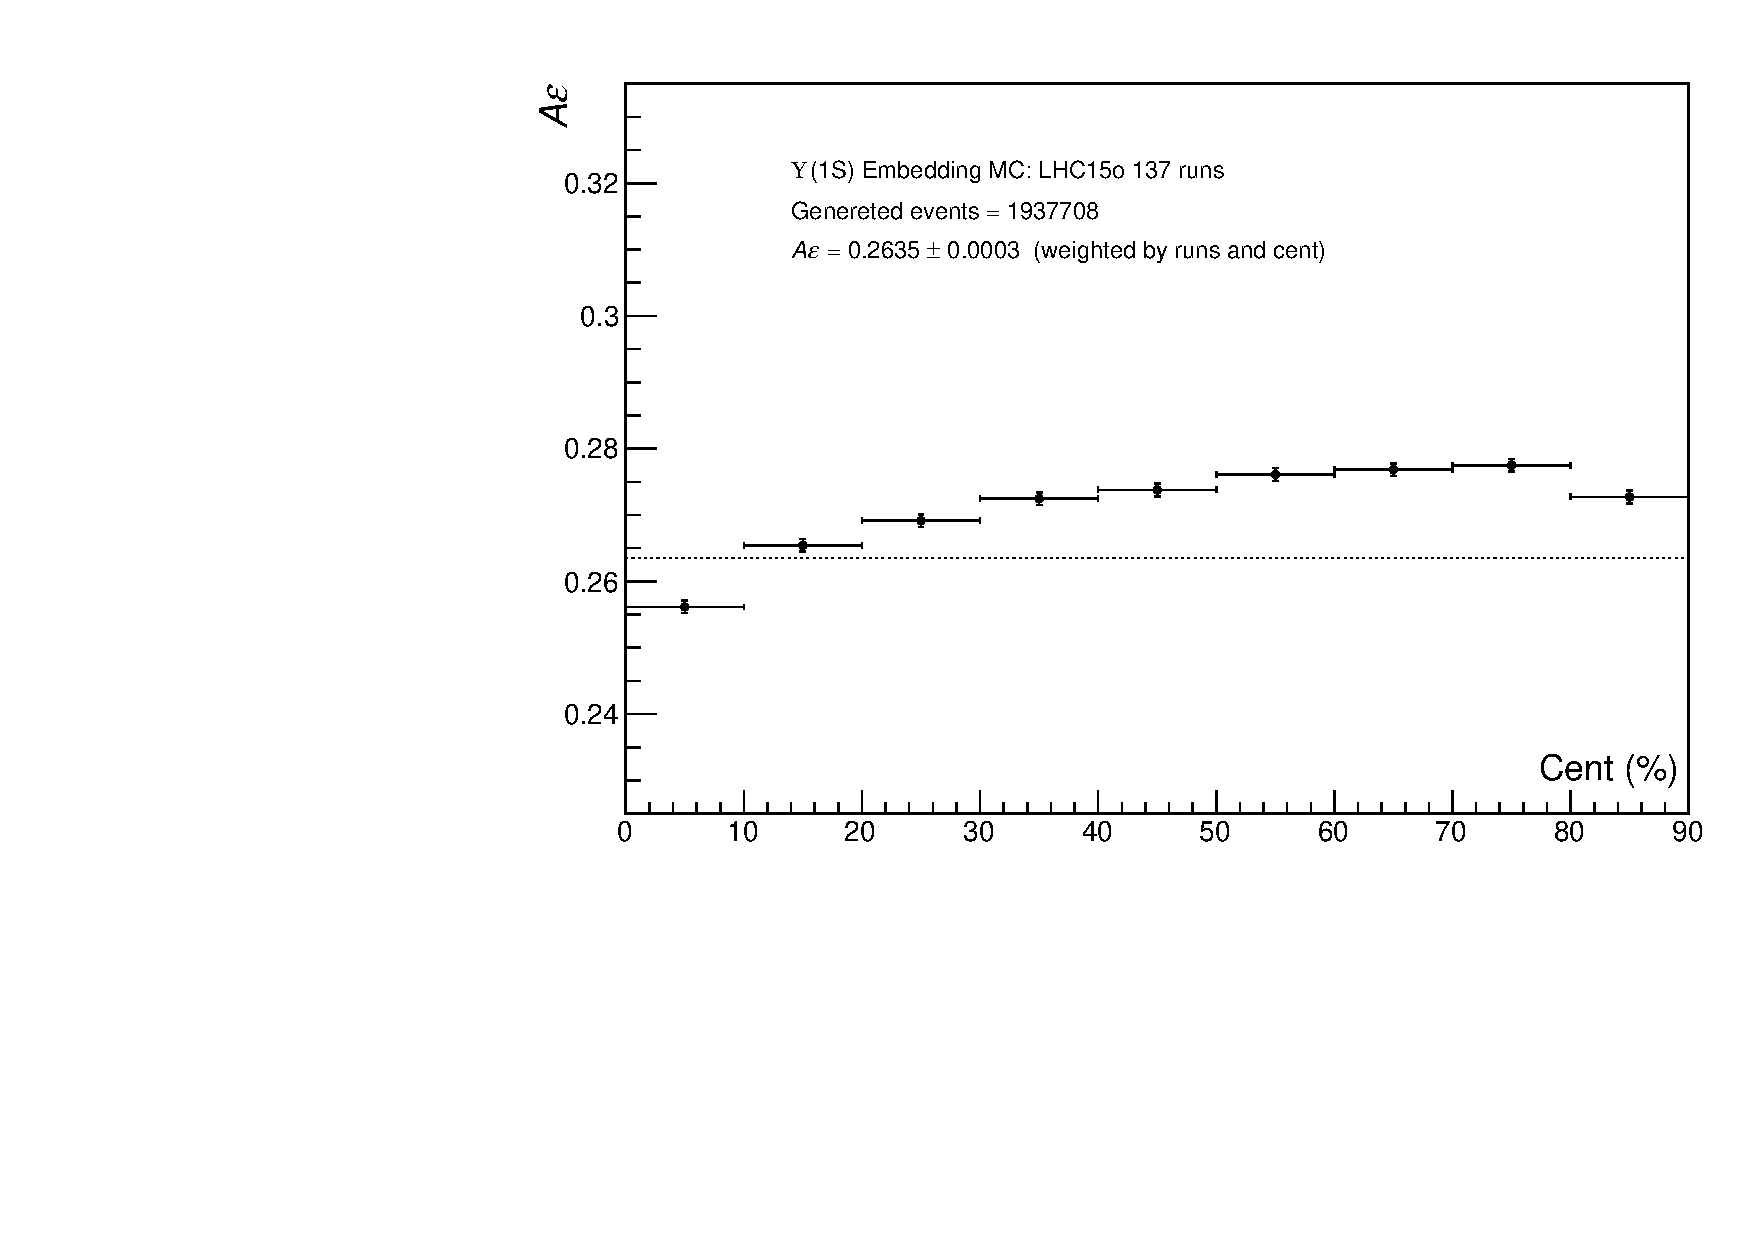
\includegraphics[width=.5\textwidth]{Chapters/Analysis/Figs/Axe/AccEffvsCent.pdf}\hfill
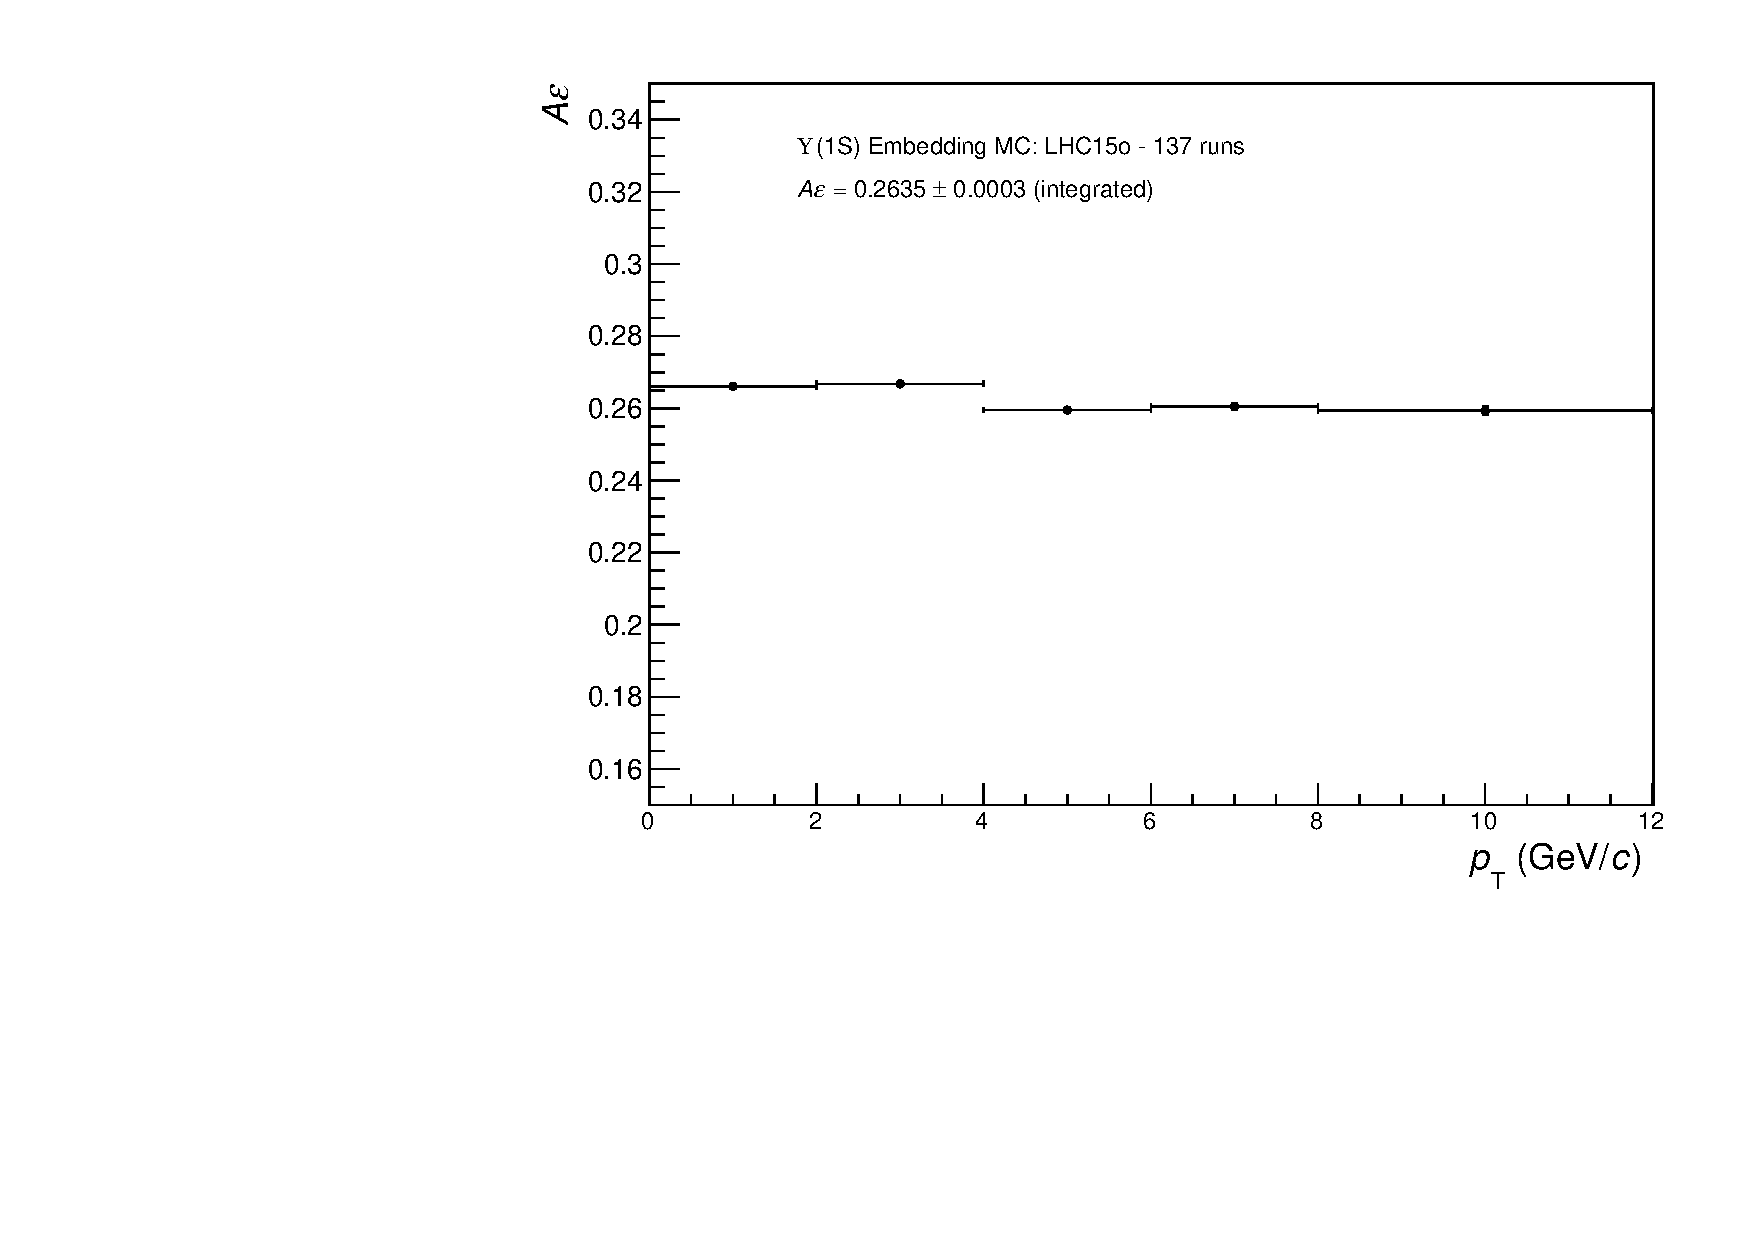
\includegraphics[width=.5\textwidth]{Chapters/Analysis/Figs/Axe/AccEffvsPt.pdf}\hfill
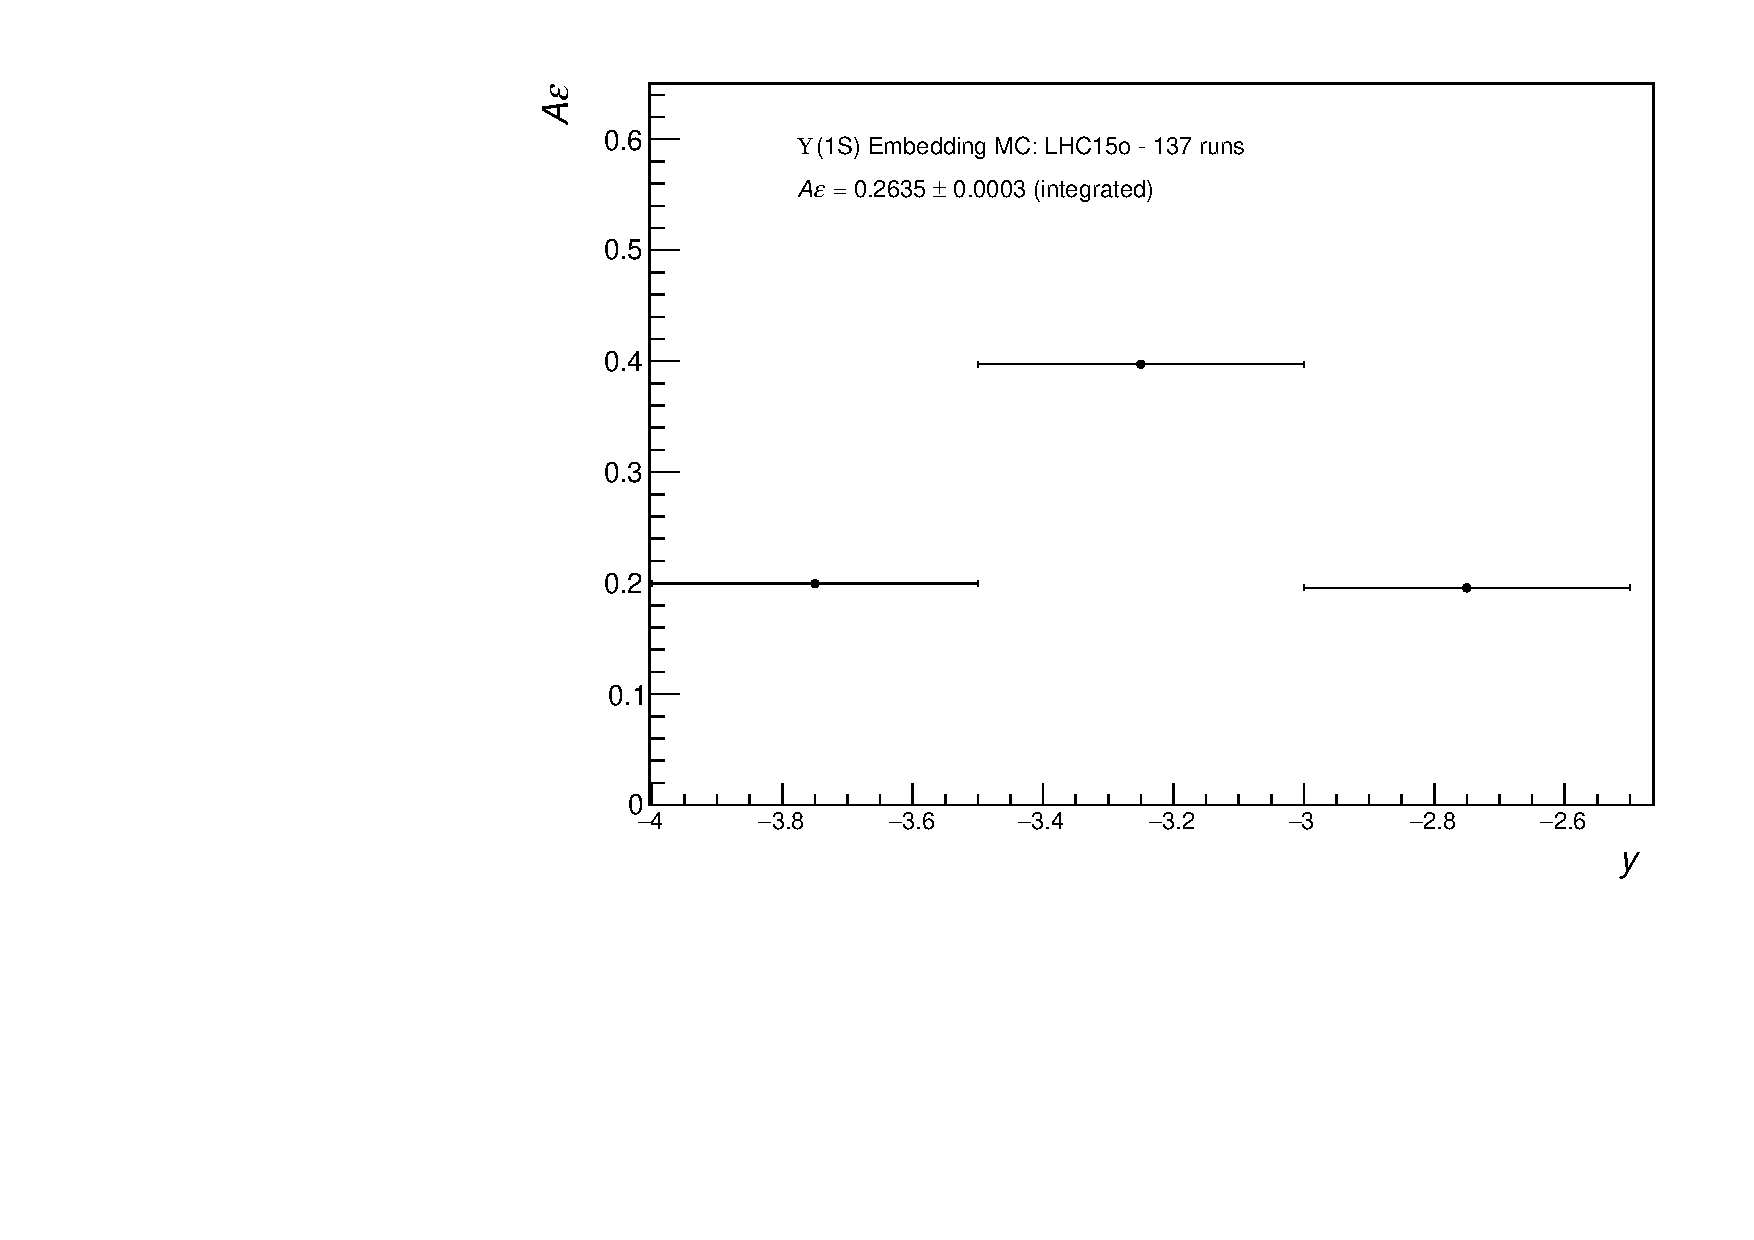
\includegraphics[width=.5\textwidth]{Chapters/Analysis/Figs/Axe/AccEffvsY.pdf}

\caption{$A\times\epsilon$ as a function of centrality (left), \pt (center), and $y$ (right). The values have been computed using embedded Monte Carlo events.}
\label{fig:Axe}

\end{figure}

% One of the ingredients appearing in the nuclear modification factor definition reported in equation \ref{eqn:raa} is the $A\times\epsilon$ correction.
The extracted number of Upsilon must be corrected by the product of the acceptance and efficiency of the detector ($A\times\epsilon$).
This correction is needed to turn the raw spectrum into one that contains physics information.
Acceptance and efficiency of each detector are evaluated through custom MC simulations.
In particular the so called "embedded" simulations are used for this studies.
In such MC simulations, the generated \upsi is embedded in a real recorded event.
This allows one to test the efficiency of detection of the simulated signal in a real event, with the full multiplicity observed in real data.
This simulation can be used for efficiency studies as well as for the acceptance ones.
% Two kinds of simulations are performed:
% \begin{itemize}
% \item Standard MC simulations: the whole event is generated by the generator and then reconstructed. The overall multiplicity is limited and this kind of simulations is useful for acceptance studies;
% \item Embedded MC simulations: the generated \upsi is embedded in a real recorded event.  This allows to test the efficiency of detection of the simulated signal in a real event, with the full multiplicity observed in real data. This simulation can be used for efficiency studies.
% \end{itemize}
Some inputs have to be provided to the MC generator.
The simulation input consists of a parameterization of the bottomonium \pt and $y$ distribution obtained by interpolating existing $pp$ measurements \cite{Acosta:2001gv,LHCb:2012aa,Khachatryan:2010zg} with the procedure described in \cite{Bossu:2011qe}.
% In particular the \pt and $y$ distributions of the generated \upsi are obtained from existing $pp$ measurements ~\cite{Acosta:2001gv,LHCb:2012aa,Khachatryan:2010zg} using the interpolation and extrapolation procedure described in~\cite{Bossu:2011qe}. 
The EKS98 nuclear shadowing parameterization~\cite{Eskola:1998df} is used to include an estimate of CNM effects.
Since available data favor a small or null polarization for $\Upsilon$(1S)~\cite{Abazov:2008aa,CDF:2011ag,Chatrchyan:2012woa}, an unpolarized production was assumed. 
The variations of the performance of the muon tracker and muon trigger systems throughout the data-taking period as well as the residual misalignment of the tracking chambers are taken into account in the simulation.

The $A\times\epsilon$ values, for the range $p_{\rm T} < 15$ GeV/$c$, $2.5 < y < 4$ and the 0--90\% centrality class are $0.263$ and $0.264$ for the \upsis and \upsiss, respectively. 
A decrease of $0.02$ is observed in  $A\times\epsilon$ for the 0--10\% central collisions with respect to the 50--90\%. 
This effect is due to a limitation of the Muon Trigger related to the higher occupancy in the most central events.
In fact the Muon Trigger LBs can provide only one tracklet each, hence if two muons cross the same LB only one of the two particles is correctly reconstructed.
Further details are given in section \ref{MTR_tagging}.
Differential studies of $A\times\epsilon$ are presented in the plots reported in figure \ref{fig:Axe}.

\section{Reference pp cross section}
\label{sec:ppxsection}
The evaluation of \raa requires to divide the yield measured in Pb-Pb collisions by the cross-section measured in $pp$ collisions at the same energy.
The statistics of the ALICE measurement at $\sqrt{s}=5.02$ in $pp$ collisions was not sufficient to provide an estimate of the \upsi cross section \cite{Adam:2016rdg}.
For this reason the reference proton-proton cross sections, for \upsis and \upsiss production, have been computed by means of an interpolation procedure described below.
The energy interpolation for the \upsi cross section, as a function of rapidity and for the \pt and $y$ integrated result, uses the measurements of \upsi production cross sections in \pp collisions at $\sqrt{s}=7$ and $8$ \rm{TeV} by ALICE \cite{Abelev:2014qha,Adam:2015rta} and at $\sqrt{s}=2.76, 7$ and $8$ \rm{TeV} by LHCb \cite{Aaij:2014nwa,Aaij:2015awa}. 
In order to obtain the reference cross section in the same \pt and $y$ bins as the ones used for the analysis, measurements from LHCb in finer \pt and $y$ bins have been combined.
The obtained values for different \pt intervals, coming from LHCb data only, are reported in tables \ref{table:LHCbData276}, \ref{table:LHCbData7} and \ref{table:LHCbData8}.
The obtained values in different $y$ bins, obtained combining both ALICE and LHCb results, are reported in tables \ref{table:LHCbY1sData276}, \ref{table:LHCbY1sData7}, \ref{table:ALICEY1sData7}, \ref{table:LHCbY1sData8} and \ref{table:ALICEY1sData8}.

\begin{table}[htp]
\begin{center}
\begin{tabular}{|c||c|c|c|c|c|c|}
  \hline
  \multicolumn{7}{|c|}{$\sqrt{s_{pp}}=$ 2.76 TeV, $2.5<y<4.0$}\\
  \hline
  $p_\mathrm{T}$ bin & $\sigma_{pp}^{\Upsilon\rightarrow \mu^{+}\mu^{\--}} $ & Stat. & uncorr. Syst. & fully corr. Syst. & Total & Relative \\
  \hline
  GeV/c & \multicolumn{5}{c|}{pb} & $\%$ \\
  \hline
  $0.0 < p_\mathrm{T} < 2.0 $ & 154,2 & 12,6 & 0,0 & 6,6 & 14,2 & 9,2 \\
  \hline
  $2.0 < p_\mathrm{T} < 4.0 $& 192,6 & 12,8 & 0,0	 & 9,6 & 16,0 & 8,3\\
  \hline
  $4.0 < p_\mathrm{T} < 6.0 $& 166,2 & 13,8 & 0,0	 & 7,8 & 15,9 & 9,5\\
  \hline
  $6.0 < p_\mathrm{T} < 15.0 $& 153,0 & 12,4	 & 0,0 & 6,6 & 14,0 & 9,2\\
  \hline
\end{tabular}
\caption{Reference cross sections and corresponding uncertainties in different $p_\mathrm{T}$ intervals. $\sigma_{pp}^{\Upsilon\rightarrow \mu^{+}\mu^{\--}} $ values and uncertainties as obtained using LHCb $pp$ data at $\sqrt{s_{pp}}=$ 2.76 TeV.}\label{table:LHCbData276}
\end{center}
\end{table}

\begin{table}[htp]
\begin{center}
\begin{tabular}{|c||c|c|c|c|c|c|}
  \hline
  \multicolumn{7}{|c|}{$\sqrt{s_{pp}}=$ 7 TeV, $2.5<y<4.0$}\\
  \hline
  $p_\mathrm{T}$ bin & $\sigma_{pp}^{\Upsilon\rightarrow \mu^{+}\mu^{\--}} $ & Stat. & uncorr. Syst. & fully corr. Syst. & Total & Relative \\
  \hline
  GeV/c & \multicolumn{5}{c|}{pb} & $\%$ \\
  \hline
  $0.0 < p_\mathrm{T} < 2.0 $ & 278,750 & 0,917 & 1,078 & 8,641 & 8,756 & 3,141 \\
  \hline
  $2.0 < p_\mathrm{T} < 4.0 $& 497,600 & 1,311 & 1,105 & 15,426 & 15,521 & 3,119 \\
  \hline
  $4.0 < p_\mathrm{T} < 6.0 $& 385,600 & 1,068 & 1,054 & 11,954 & 12,047 & 3,124 \\
  \hline
  $6.0 < p_\mathrm{T} < 15.0 $& 473,720 & 1,197 & 0,936 & 14,685 & 14,764 & 3,117 \\
  \hline
\end{tabular}
\caption{Reference cross sections and corresponding uncertainties in different $p_\mathrm{T}$ intervals. $\sigma_{pp}^{\Upsilon\rightarrow \mu^{+}\mu^{\--}} $ values and uncertainties as obtained using LHCb $pp$ data at $\sqrt{s_{pp}}=$ 7 TeV.}\label{table:LHCbData7}
\end{center}
\end{table}

\begin{table}[htp]
\begin{center}
\begin{tabular}{|c||c|c|c|c|c|c|}
  \hline
  \multicolumn{7}{|c|}{$\sqrt{s_{pp}}=$ 8 TeV, $2.5<y<4.0$}\\
  \hline
  $p_\mathrm{T}$ bin & $\sigma_{pp}^{\Upsilon\rightarrow \mu^{+}\mu^{\--}} $ & Stat. & uncorr. Syst. & fully corr. Syst. & Total & $\%$ \\
  \hline
  GeV/c & \multicolumn{5}{c|}{pb} & $\%$ \\
  \hline
  $0.0 < p_\mathrm{T} < 2.0 $ & 337.680 & 0.811 & 0.967 & 9.455 & 9.539 & 2.825 \\
  \hline
  $2.0 < p_\mathrm{T} < 4.0 $& 610.400 & 1.068 & 1.367 & 17.091 & 17.179 & 2.814 \\
  \hline
  $4.0 < p_\mathrm{T} < 6.0 $& 481.000 & 0.906 & 1.010 & 13.468 & 13.536 & 2.814 \\
  \hline
  $6.0 < p_\mathrm{T} < 15.0 $& 609.970 & 1.022 & 0.905 & 17.079 & 17.134 & 2.809 \\
  \hline
\end{tabular}
\caption{Reference cross sections and corresponding uncertainties in different $p_\mathrm{T}$ intervals. $\sigma_{pp}^{\Upsilon\rightarrow \mu^{+}\mu^{\--}} $ values and uncertainties as obtained using LHCb $pp$ data at $\sqrt{s_{pp}}=$ 8 TeV.}\label{table:LHCbData8}
\end{center}
\end{table}

\begin{table}[!tp]
\begin{center}
\begin{tabular}{|c||c|c|c|c|c|c|}
  \hline
  \multicolumn{7}{|c|}{$\sqrt{s_{pp}}=$ 2.76 TeV, $0<p_\mathrm{T}<15$}\\
  \hline
  $y$ bin & $d(\sigma_{pp}^{\Upsilon\rightarrow \mu^{+}\mu^{\--}})/dy $ & Stat. & uncorr. Syst. & fully corr. Syst. & Total & $\%$ \\
  \hline
  GeV/c & \multicolumn{5}{c|}{pb} & $\%$ \\
  \hline
  $2.5 < y < 3.0 $ & 642 & 36 & 0 & 24 & 43 & 7 \\
  \hline
  $3.0 < y < 3.5 $& 454 & 26 & 0 & 16 & 31 & 7 \\
  \hline
  $3.5 < y < 4.0 $& 248 & 22 & 0 & 10 & 24 & 10 \\
  \hline
  $2.5 < y < 4.0 $& 448 & 17 & 0 & 16 & 24 & 5 \\
  \hline
\end{tabular}
\caption{$y$ bins $d(\sigma_{pp}^{\Upsilon\rightarrow \mu^{+}\mu^{\--}})/dy $ values and uncertainties as obtained using LHCb $pp$ data at $\sqrt{s_{pp}}=$ 2,76 TeV.}\label{table:LHCbY1sData276}
\end{center}
\end{table}

\begin{table}[!tp]
\begin{center}
\begin{tabular}{|c||c|c|c|c|c|c|}
  \hline
  \multicolumn{7}{|c|}{$\sqrt{s_{pp}}=$ 7 TeV, $0<p_\mathrm{T}<15$}\\
  \hline
  $y$ bin & $d(\sigma_{pp}^{\Upsilon\rightarrow \mu^{+}\mu^{\--}})/dy $ & Stat. & uncorr. Syst. & fully corr. Syst. & Total & $\%$ \\
  \hline
  GeV/c & \multicolumn{5}{c|}{pb} & $\%$ \\
  \hline
  $2.5 < y < 3.0 $ & 1291.40 & 2.96 & 2.08 & 40.20 & 40.36 & 3.1 \\
  \hline
  $3.0 < y < 3.5 $& 1116.58 & 2.48 & 2.04 & 34.76 & 34.91 & 3.1 \\
  \hline
  $3.5 < y < 4.0 $& 863.36 & 2.40 & 2.98 & 27.04 & 27.31 & 3.2 \\
  \hline
  $2.5 < y < 4.0 $& 1090.45 & 4.55 & 4.17 & 33.80 & 34.36 & 3.2 \\
  \hline
\end{tabular}
\caption{$y$ bins $d(\sigma_{pp}^{\Upsilon\rightarrow \mu^{+}\mu^{\--}})/dy $ values and uncertainties as obtained using LHCb $pp$ data at $\sqrt{s_{pp}}=$ 7 TeV.}\label{table:LHCbY1sData7}
\end{center}
\end{table}

\begin{table}[!tp]
\begin{center}
\begin{tabular}{|c||c|c|c|c|c|c|}
  \hline
  \multicolumn{7}{|c|}{$\sqrt{s_{pp}}=$ 8 TeV, $0<p_\mathrm{T}<15$}\\
  \hline
  $y$ bin & $d(\sigma_{pp}^{\Upsilon\rightarrow \mu^{+}\mu^{\--}})/dy $ & Stat. & uncorr. Syst. & fully corr. Syst. & Total & $\%$ \\
  \hline
  GeV/c & \multicolumn{5}{c|}{pb} & $\%$ \\
  \hline
  $2.5 < y < 3.0 $ & 1659.32 & 2.50 & 2.44 & 46.60 & 46.73 & 2.8 \\
  \hline
  $3.0 < y < 3.5 $& 1370.82 & 2.04 & 2.66 & 38.52 & 38.67 & 2.8 \\
  \hline
  $3.5 < y < 4.0 $& 1047.96 & 2.06 & 2.34 & 29.50 & 29.66 & 2.8 \\
  \hline
  $2.5 < y < 4.0 $& 1359.37 & 3.83 & 4.30 & 38.06 & 38.50 & 2.8 \\
  \hline
\end{tabular}
\caption{$y$ bins $d(\sigma_{pp}^{\Upsilon\rightarrow \mu^{+}\mu^{\--}})/dy $ values and uncertainties as obtained using LHCb $pp$ data at $\sqrt{s_{pp}}=$ 8 TeV.}\label{table:LHCbY1sData8}
\end{center}
\end{table}

\begin{table}[!tp]
\begin{center}
\begin{tabular}{|c||c|c|c|c|c|c|}
  \hline
  \multicolumn{7}{|c|}{$\sqrt{s_{pp}}=$ 7 TeV, $0<p_\mathrm{T}<12$}\\
  \hline
  $y$ bin & $d(\sigma_{pp}^{\Upsilon\rightarrow \mu^{+}\mu^{\--}})/dy $ & Stat. & uncorr. Syst. & fully corr. Syst. & Total & $\%$ \\
  \hline
  GeV/c & \multicolumn{5}{c|}{pb} & $\%$ \\
  \hline
  $2.5 < y < 3.0 $ & 1158.16 & 183.52 & 151.52 & 58.03 & 244.81 & 21.1 \\
  \hline
  $3.0 < y < 3.5 $& 944.88 & 143.84 & 163.68 & 47.37 & 222.99 & 23.6 \\
  \hline
  $3.5 < y < 4.0 $& 607.60 & 124.00 & 81.84 & 30.50 & 151.67 & 25.0 \\
  \hline
  $2.5 < y < 4.0 $& 896.11 & 82.67 & 110.77 & 44.81 & 145.30 & 17.2 \\
  \hline
\end{tabular}
\caption{$y$ bins $d(\sigma_{pp}^{\Upsilon\rightarrow \mu^{+}\mu^{\--}})/dy $ values and uncertainties as obtained using ALICE $pp$ data at $\sqrt{s_{pp}}=$ 7 TeV.}\label{table:ALICEY1sData7}
\end{center}
\end{table}

\begin{table}[!tp]
\begin{center}
\begin{tabular}{|c||c|c|c|c|c|c|}
  \hline
  \multicolumn{7}{|c|}{$\sqrt{s_{pp}}=$ 8 TeV, $0<p_\mathrm{T}<12$}\\
  \hline
  $y$ bin & $d(\sigma_{pp}^{\Upsilon\rightarrow \mu^{+}\mu^{\--}})/dy $ & Stat. & uncorr. Syst. & fully corr. Syst. & Total & $\%$ \\
  \hline
  GeV/c & \multicolumn{5}{c|}{pb} & $\%$ \\
  \hline
  $2.5 < y < 3.0 $ & 1669.04 & 270.32 & 143.84 & 83.45 & 317.38 & 19.0 \\
  \hline
  $3.0 < y < 3.5 $& 1173.04 & 136.40 & 91.76 & 58.65 & 174.54 & 14.9 \\
  \hline
  $3.5 < y < 4.0 $& 806.00 & 161.20 & 89.28 & 40.30 & 188.63 & 23.4 \\
  \hline
  $2.5 < y < 4.0 $& 1173.87 & 99.20 & 115.73 & 58.69 & 163.34 & 13.9 \\
  \hline
\end{tabular}
\caption{$y$ bins $d(\sigma_{pp}^{\Upsilon\rightarrow \mu^{+}\mu^{\--}})/dy $ values and uncertainties as obtained using ALICE $pp$ data at $\sqrt{s_{pp}}=$ 8 TeV.}\label{table:ALICEY1sData8}
\end{center}
\end{table}

The energy interpolation is performed fitting the experimental data using the empirical functions listed below:
\begin{itemize}
    \item Linear function: $p_0+p_1\cdot\sqrt{s}$
    \item Parabola: $p_0\cdot\sqrt{s}+p_1\cdot(\sqrt{s})^2$
    \item Positive exponential: $p_0\cdot\sqrt{s}\cdot e^{\frac{\sqrt{s}}{p_1}}$
    \item Negative exponential: $p_0\cdot(1-e^{\frac{-\sqrt{s}}{p_1}})$
    \item Power law: $p_0\cdot(\sqrt{s})^{p_1}$
\end{itemize}
The requirement for such functions is to be able to intercept the origin of the axes.
This choice is driven by the convincing assumption that at $\sqrt{s}=0$ \rm{TeV}  the cross-section drops to $0$.
% In addition to the functions satisfying this requirement, representing the first order Taylor expansion of any other functional form, a straight line has been added to the set of interpolating functions.
The energy interpolation for the \upsis cross section as a function of \pt is based on LHCb measurements only, since the  \pt coverage of the results of this analysis ($p_{\rm T} < 15$ GeV/$c$) is more extended than that of the corresponding ALICE $pp$ data ($p_{\rm T} < 12$ GeV/$c$).
The plots representing the data points, the interpolation functions and the interpolated values are shown in figure \ref{fig:sigmapp}.

\begin{figure}[!b]
\begin{center}
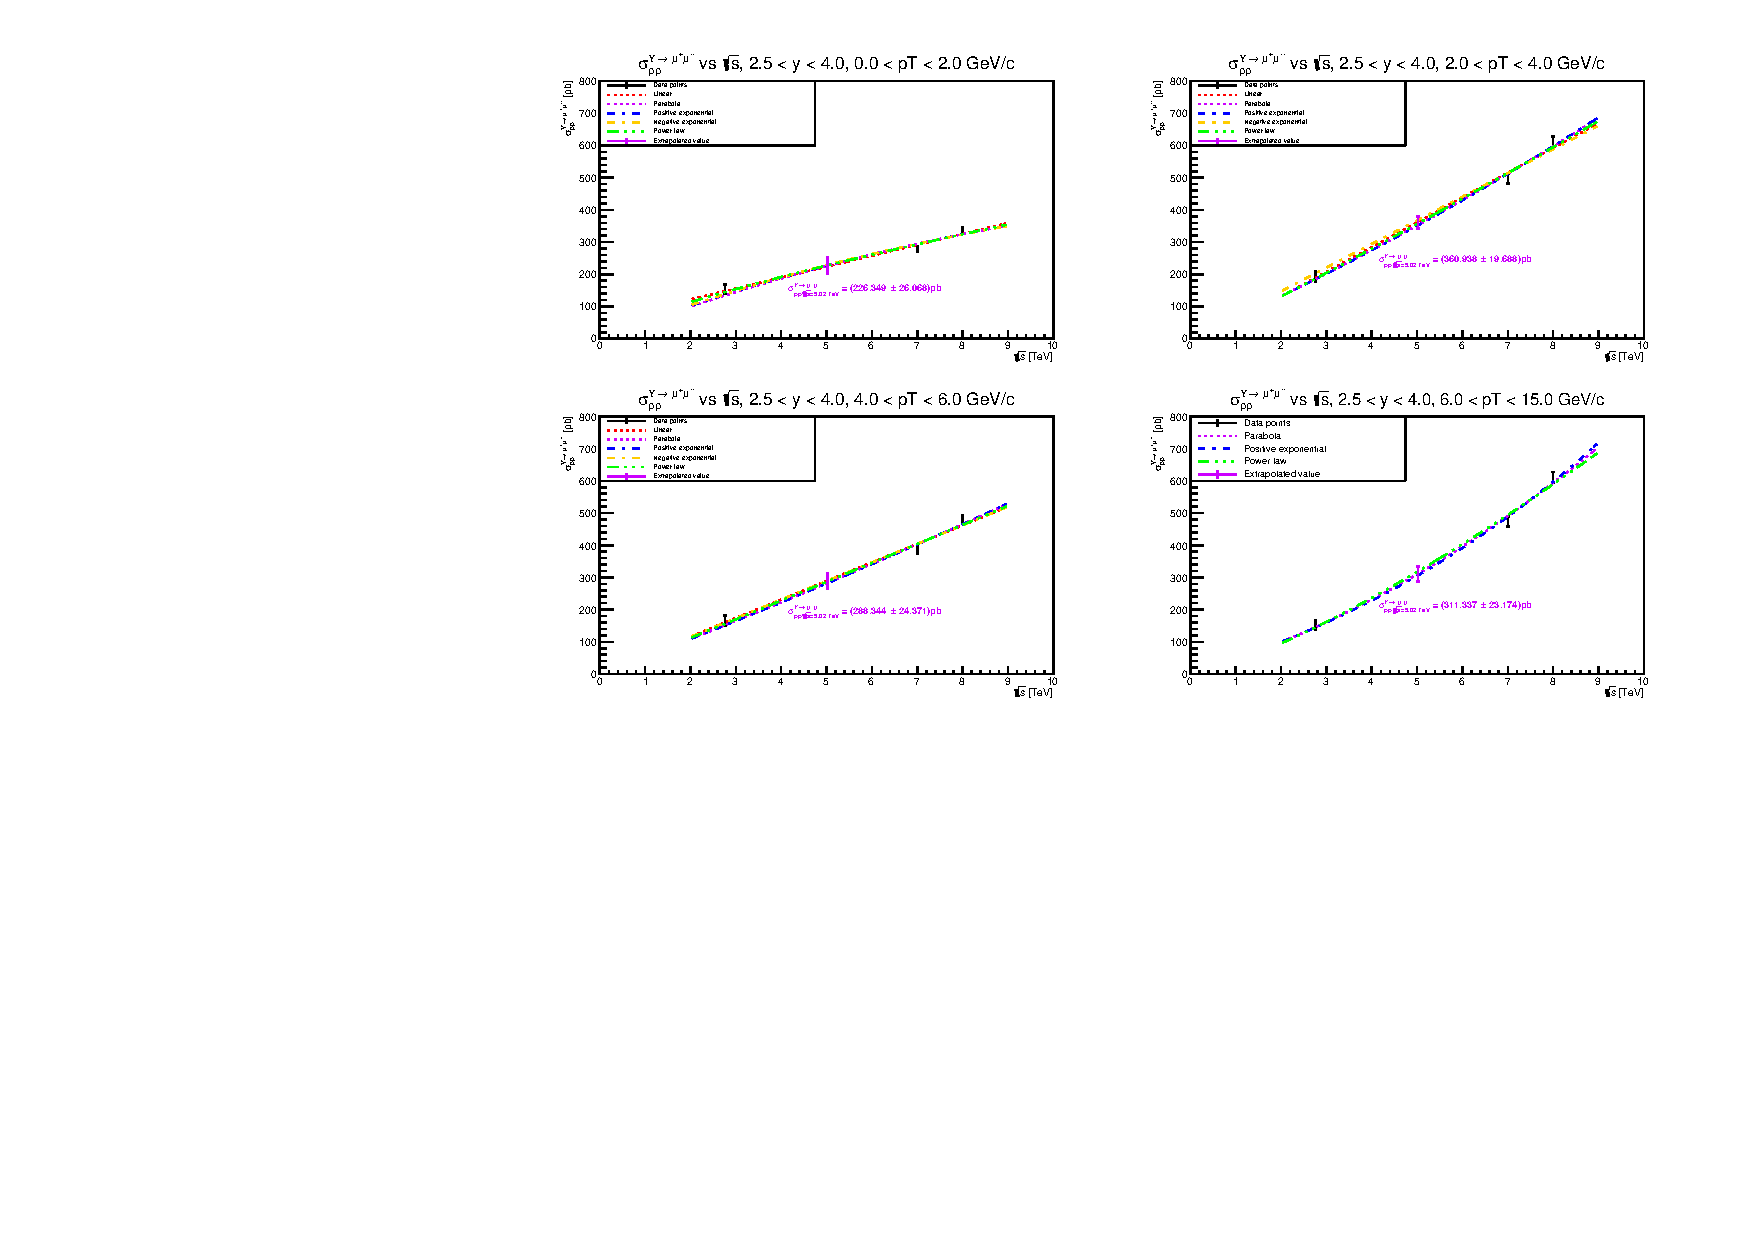
\includegraphics[width=0.95\linewidth]{Chapters/Analysis/Figs/sigmapp_vs_pt.pdf}
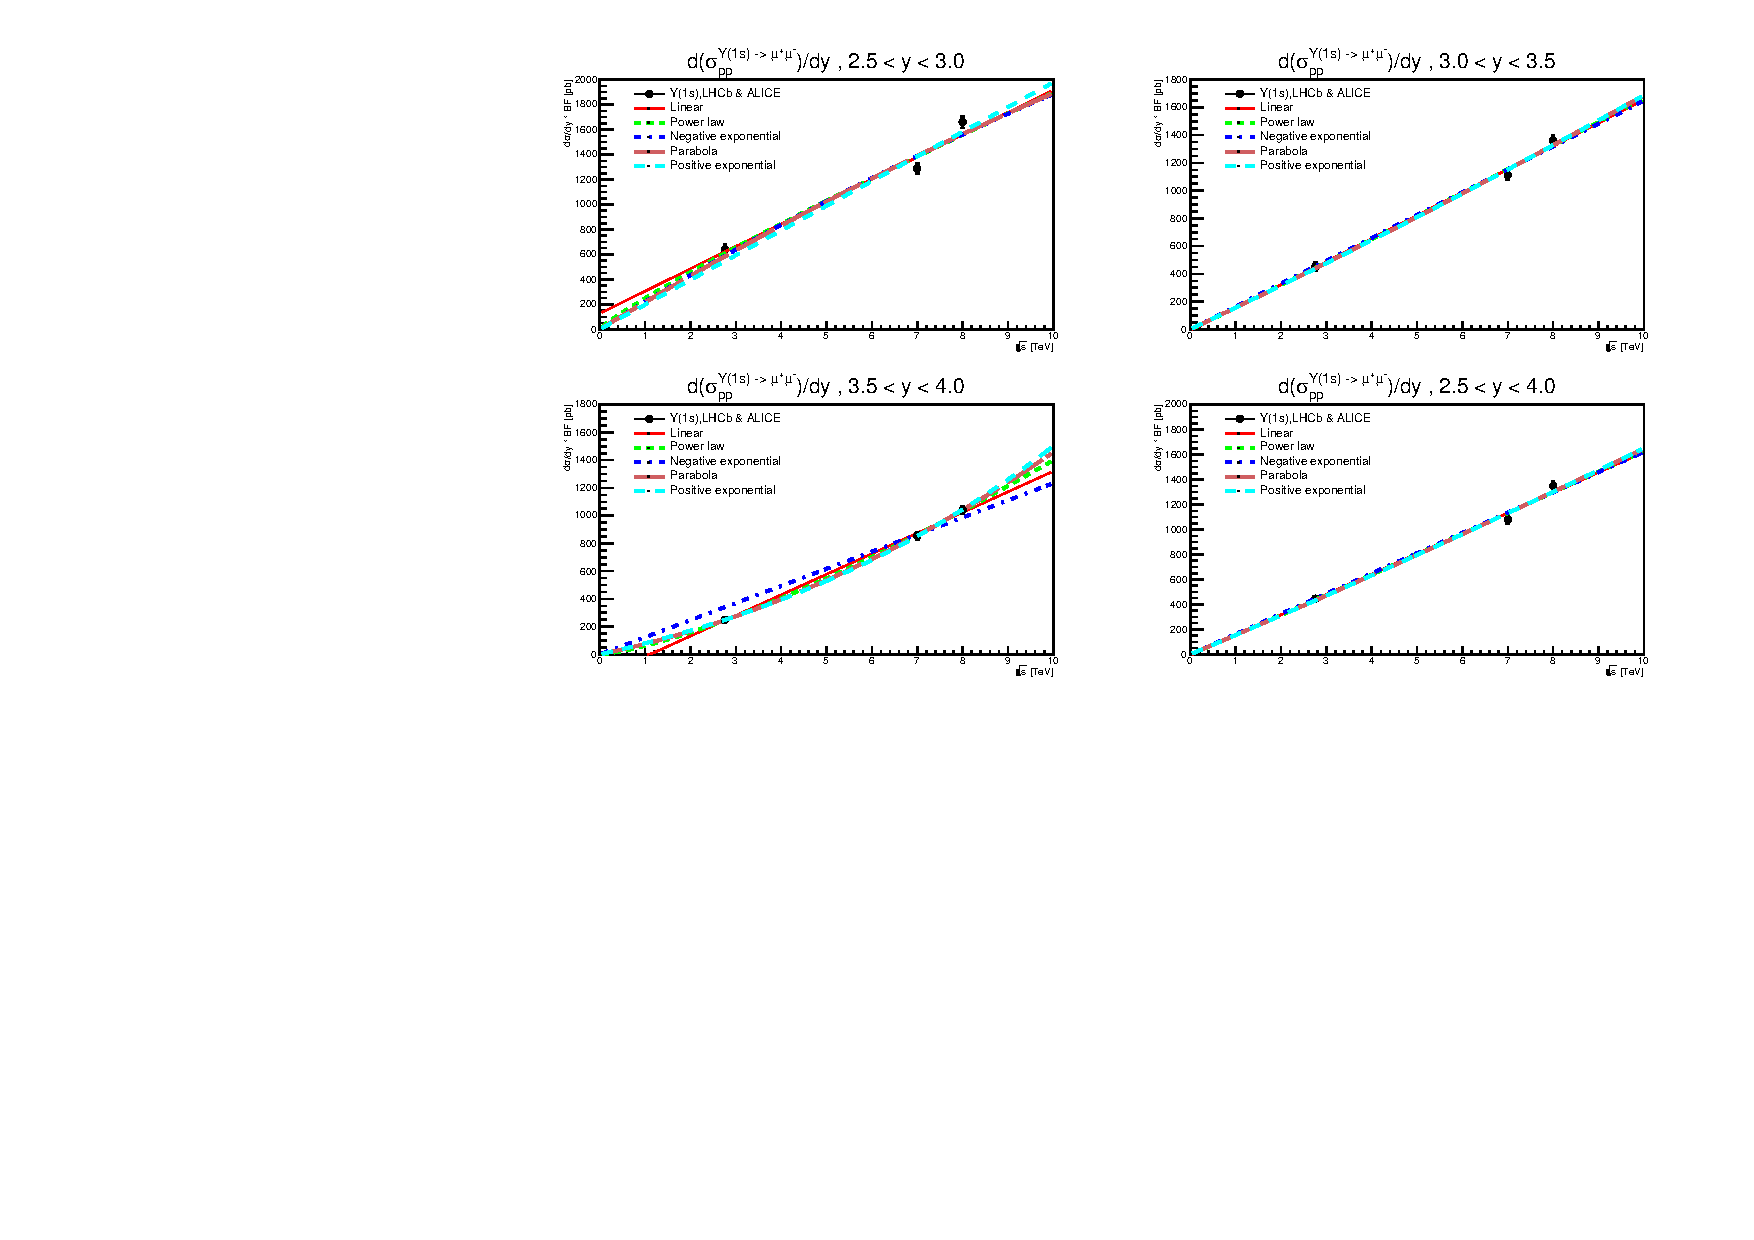
\includegraphics[width=0.95\linewidth]{Chapters/Analysis/Figs/sigmapp_vs_y.pdf}
\caption{Interpolation of reference $\sigma_{pp}$ in \pt (top 4 graphs) and $y$ (bottom 4 graphs) bins. The measured points are reported with an error bar that is the quadratic sum of the statistical and systematic uncertainties.}
\label{fig:sigmapp}
\end{center}
\end{figure}

The final cross section value is the weighted average of the whole set of interpolated values.
The total uncertainty on the interpolated $pp$ cross-section corresponds to the quadratic sum of two terms. 
One term represents the statistical uncertainty and reflects the uncertainties on the data samples used in the interpolation procedure.
% This term is the uncertainty on the average of the interpolated values using the whole set of functions and theoretical models.
The second term represents the systematic uncertainty related to the interpolation procedure itself.
It corresponds to the maximum spread between the final cross section value and each single interpolation.
The numerical values obtained from the interpolation procedure are summarized in Table~\ref{tab:ref_cs_pp} for the various kinematic ranges used in the analysis.
The result of the interpolation procedure gives ${\rm BR}_{\Upsilon\text{(1S)} \rightarrow \mu^{+} \mu^{-}} \cdot \sigma^{\rm\Upsilon({\rm 1S})}_{\rm pp}=1221\pm77\text{(tot)}$~pb and ${\rm BR}_{\Upsilon\text{(2S)} \rightarrow \mu^{+} \mu^{-}} \cdot \sigma^{\rm\Upsilon({\rm 2S})}_{\rm pp}=302\pm23\text{(tot)}$~pb assuming unpolarized quarkonia and integrating over the ranges $2.5 < y < 4$ and $p_{\rm T} < 15\ GeV/c$.
% These values differ from the sum of the differential values reported in \ref{tab:ref_cs_pp}.
% The integrated values are 

\begin{table}[!t]
\centering
\begin{tabular}{| c | c | c |}
\hline
\pt (GeV/$c$) & $y$ & ${\rm BR}_{\Upsilon\text{(1S)} \rightarrow \mu^{+} \mu^{-}} \cdot \sigma_{\rm pp}^{\Upsilon{\rm (1S)}}$ (pb) \tabularnewline
\hline 
{[}0-2{]} & \multirow{4}{*}{{[}2.5-4{]}} & $226 \pm 26$\tabularnewline
%\cline{1-1} \cline{3-3} 
{[}2-4{]} &  & $361 \pm 20$\tabularnewline
%\cline{1-1} \cline{3-3} 
{[}4-6{]} &  & $288 \pm 24$\tabularnewline
%\cline{1-1} \cline{3-3} 
{[}6-15{]} &  & $311 \pm 23$\tabularnewline
\hline 
\multirow{3}{*}{{[}0-15{]}} & {[}2.5-3{]} & $ 506 \pm 57 $\tabularnewline
%\cline{2-3} 
 & {[}3-3.5{]} & $ 415 \pm 28 $\tabularnewline
%\cline{2-3} 
 & {[}3.5-4{]} & $ 288 \pm 24$\tabularnewline
\hline 
\end{tabular}
\caption{\label{tab:ref_cs_pp} The interpolated branching ratio times cross section of \upsis for the \pt and $y$ bins under study.}
\end{table}

It should be noted that the integrals of the interpolated  $p_{\mathrm{T}}$-differential and $y$-differential  cross sections differ by at most $\approx3\%$ from the interpolated integrated cross sections. 
This indicates a good consistency of the interpolation procedure across various kinematical ranges, also considering that the uncertainties on the obtained cross sections are not completely correlated.

% % %%%%%%%%%%%%%%%%%%%%%%%%%%%%%%%%%%%%%%%%%%%%%%%%
\section{Uncertainties}\label{subsec:syst_uncert}

The systematic uncertainty on \raa has several contributions related to the various ingredients which constitute the nuclear modification definition in equation \ref{eqn:raa}.
% Several procedures have been performed to obtain such ingredients and the systematic uncertainty contribution of each of these procedures has to be evaluated and quoted alongside the final result.
The estimation of the systematic uncertainties will be detailed in the following.

The systematic uncertainty on the signal extraction is evaluated by considering the variations in the signal counts when using various functions for the description of the background for the invariant mass distribution, as well as adopting two fitting ranges, $i.e.$ $(7-14)$ GeV/$c^2$ and $(7.5-14.5)$ GeV/$c^2$.
As it has already been mentioned, the signal extraction procedure can be performed either on the raw mass spectrum or on the mass spectrum with applied event mixing subtraction.
In both cases, the resulting distribution is fitted with the sum of three extended CB and a function to account for the residual background.
The extended CB tail parameters have been varied using estimates provided by two MC transport models: GEANT4~\cite{Agostinelli:2002hh} and GEANT3~\cite{Brun:1082634}. 
Due to lack of statistics for the higher mass bottomonium resonances, the mass position and width of the \upsiss and \upsisss have been fixed to the \upsis position and width obtained from the fit, using the ratio obtained from the PDG as scaling factor.
To take in account for the statistical uncertainty on such choice, the ratio of \upsiss ($\Upsilon\text{(3S)}$) to \upsis widths is varied from 1 (1) to 1.06 (1.12).
In the centrality, \pt or $y$ differential studies, the mass position and width are also varied, by an amount which corresponds to the uncertainties on the mass position and the width returned by the fit to the integrated invariant mass spectrum. 
The central values of $N^{\Upsilon}$ and their statistical uncertainties are obtained by taking the weighted average of $N^{\Upsilon}$ and of the corresponding statistical uncertainties from the various fits.
The systematic uncertainties are estimated as the root mean square of the distribution of $N^{\Upsilon}$ obtained from the various fits.

As already reported, a cut of $p_{\rm T} > 2$ GeV/$c$ on single muons has been applied to filter out the contribution of muons from $K$ and $\pi$ decays.
The impact of such cut on signal and background can be qualitatively evaluated from the scatter plots reported in figure \ref{fig:ptcut}.

\begin{figure}[!b]
\begin{center}
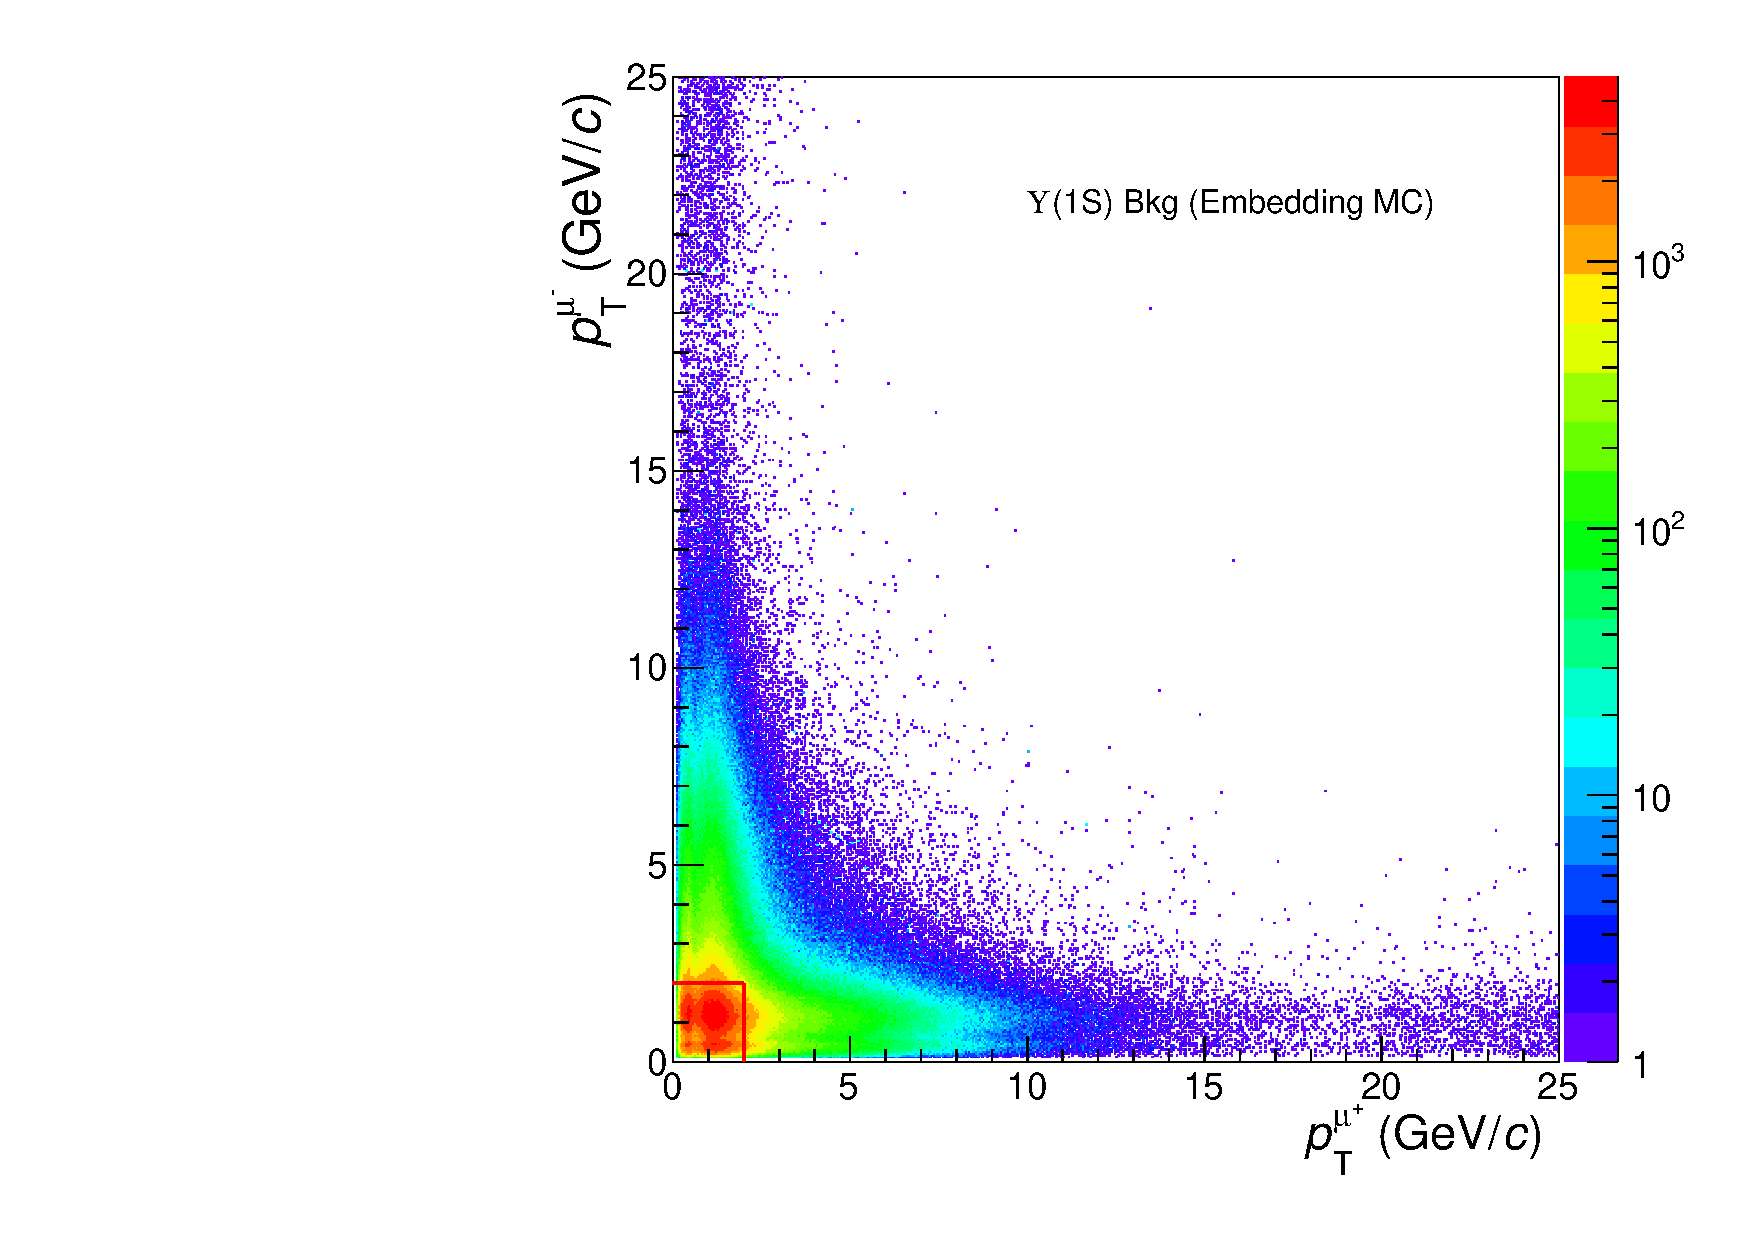
\includegraphics[width=0.45\linewidth]{Chapters/Analysis/Figs/background.pdf}
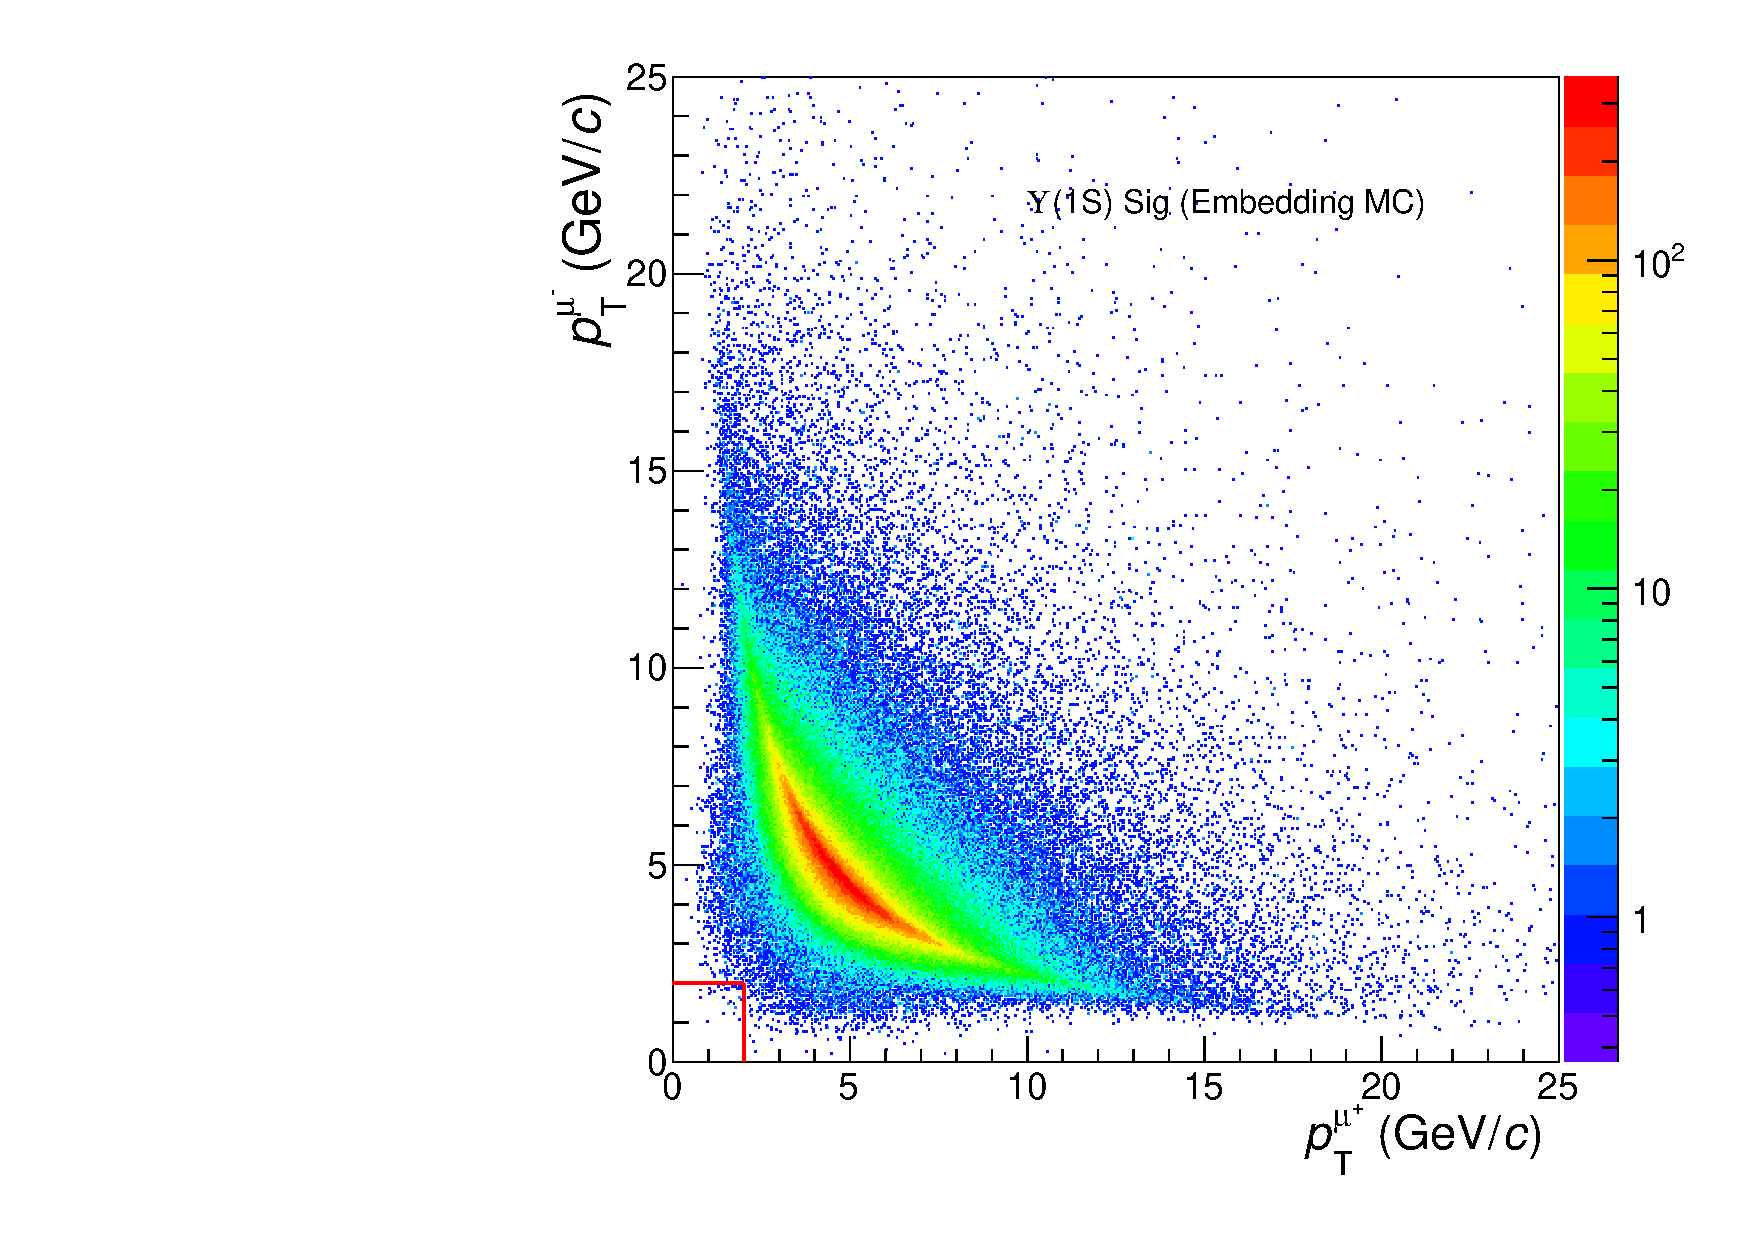
\includegraphics[width=0.45\linewidth]{Chapters/Analysis/Figs/signal.pdf}
\caption{Density plot of muon pair candidates' \pt~s for background candidates (left) and signal candidates (right). The cut at $p_{\rm{T}}=2 \rm{GeV}/c$ on both muons is represented as a red box.}
\label{fig:ptcut}
\end{center}
\end{figure}

The effect induced by that cut on \upsi yields was estimated by varying that cut by $\pm10$\%.
A $\pm2$\% maximum variation on the number of detected \upsi resonances, $N^{\Upsilon}$, was observed and included in the systematic uncertainties.

Various sources contribute to the systematic uncertainties of $A\times\epsilon$, such as input MC, the trigger efficiency, the track reconstruction efficiency and finally the matching efficiency between tracks in the muon tracking and triggering chambers. 

To evaluate the systematic uncertainty induced by the MC input shapes, various sets of simulations have been produced with different \upsi input \pt and $y$ distributions, obtained from empirical parameterizations and/or extrapolations of available data sets, such as ALICE data in \pbpb collisions at $\sqrt{s_{_{\rm NN}}}=5.02$~\rm{TeV}, $\sqrt{s_{_{\rm NN}}}=2.76$ \rm{TeV} and $pp$ collisions at $\sqrt{s}=5.02$~\rm{TeV} and CDF data in \pbpb at $\sqrt{s_{_{\rm NN}}}=4$~\rm{TeV}. 
The maximum relative difference of $A\times\epsilon$ obtained using the various input shapes is taken as the systematic uncertainty due to the MC input.
A summary of all the tests can be found in figure \ref{fig:MCsyst}.

\begin{figure}[!b]
\begin{center}
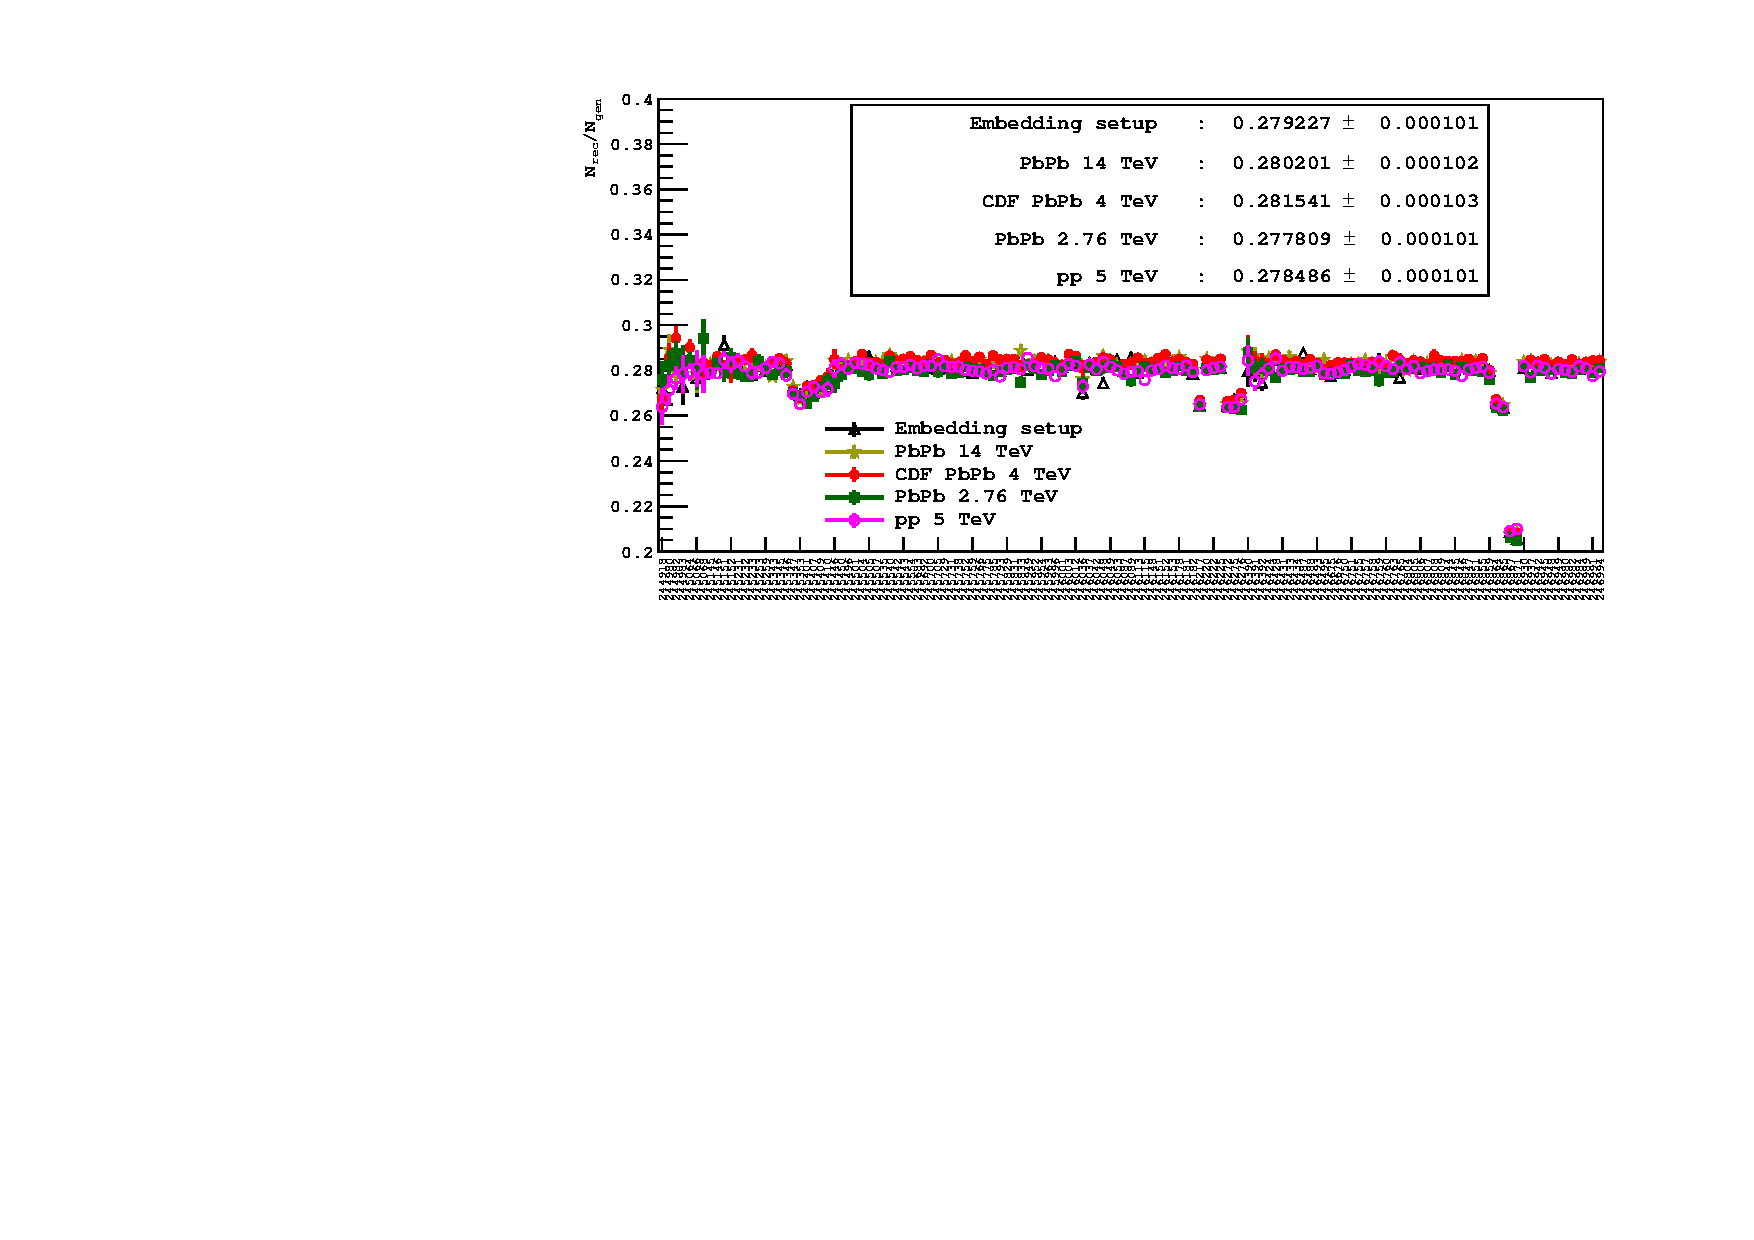
\includegraphics[width=\linewidth]{Chapters/Analysis/Figs/Axe/AxE_integrated.pdf}
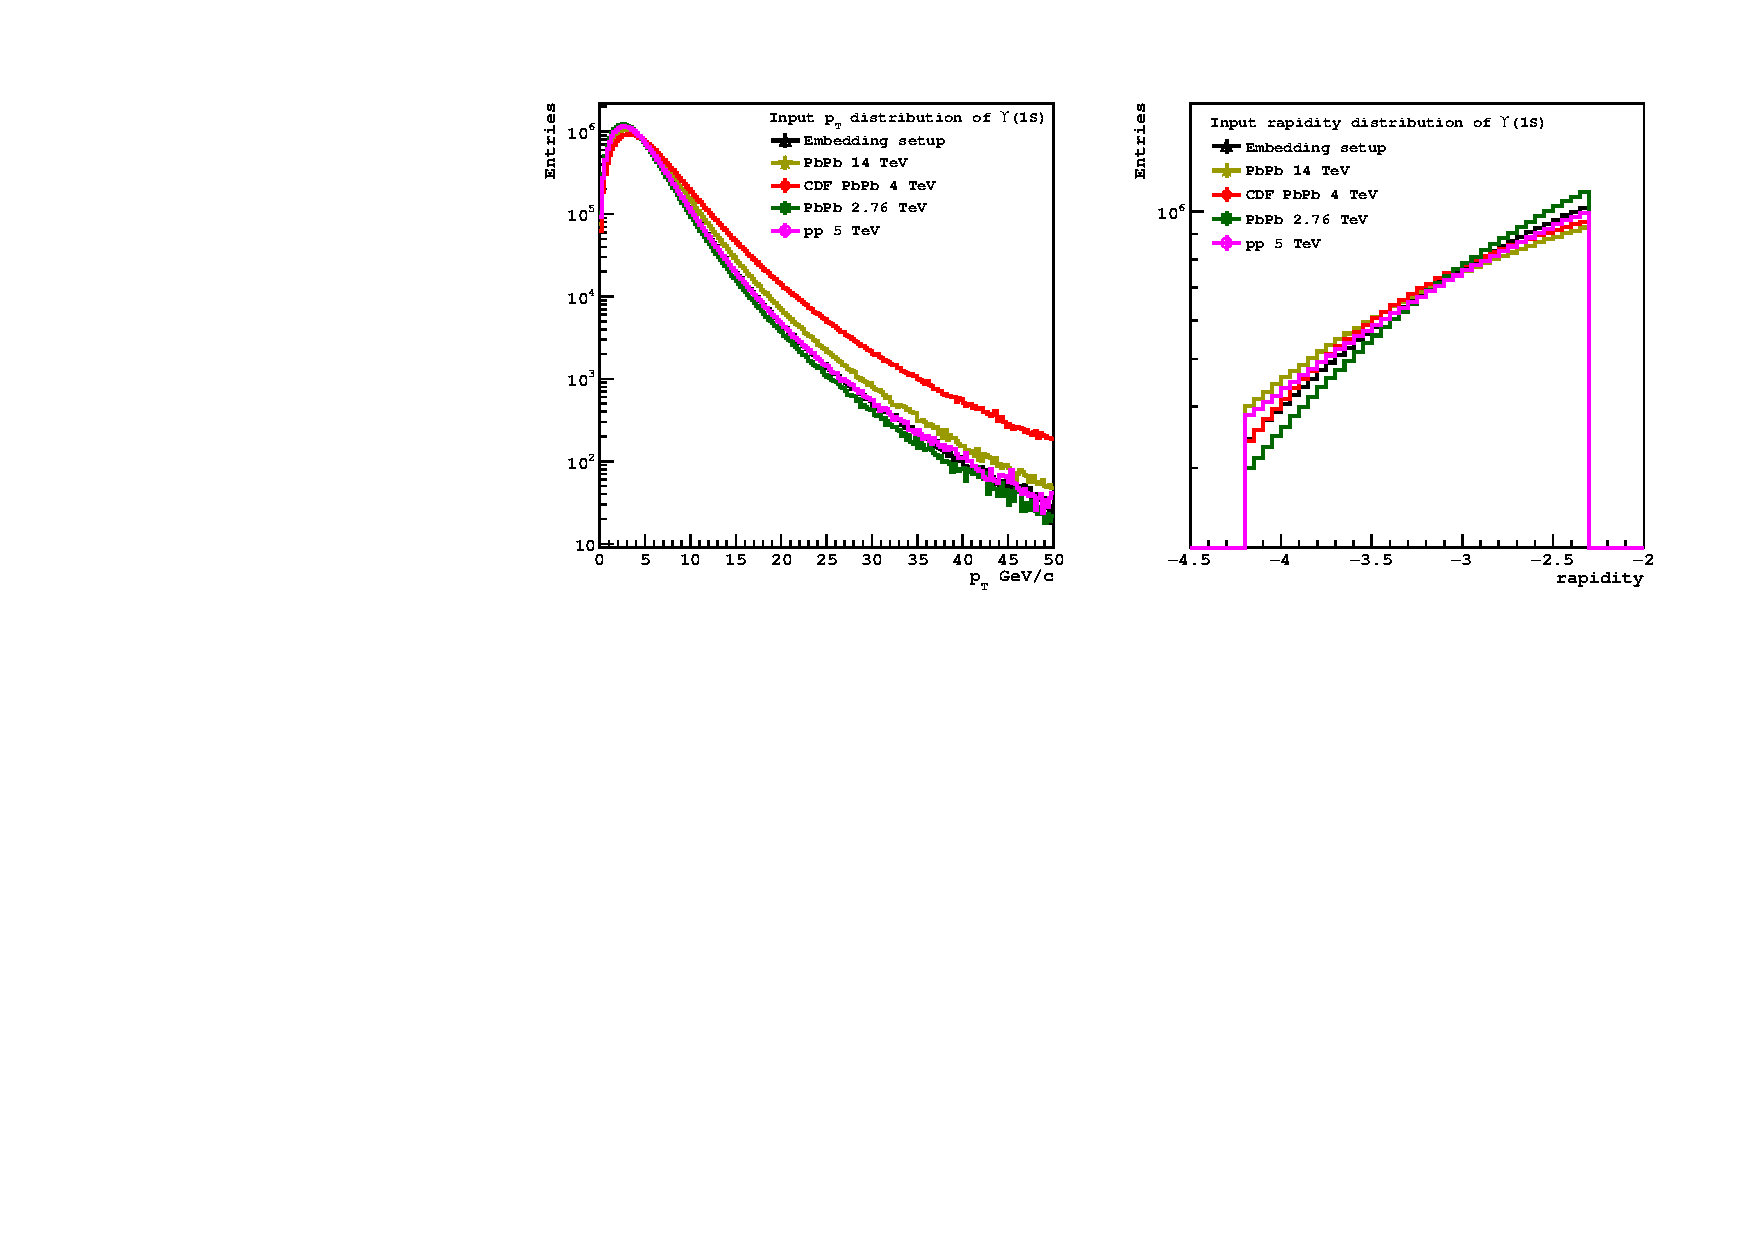
\includegraphics[width=0.9\linewidth]{Chapters/Analysis/Figs/input_pt_rap_dist.pdf}
\caption{Evolution of the $N_{rec}/N_{gen}$ ratio versus run number (top). Different colors refer to different input distributions for \upsis \pt and $y$ values, represented with the same color code in the bottom panel. Please note that the systematic study as a function of rapidity adopts an inverted convention for rapidity values, with respect to that adopted in this thesis, hence rapidity values are quoted as negative.}
\label{fig:MCsyst}
\end{center}
\end{figure}

In order to calculate the systematic uncertainty on the trigger efficiency, the trigger response function for single muons is evaluated using either MC or data.
The two response functions are then separately applied to simulations of a \upsi sample and the difference obtained for the \upsi reconstruction efficiency is taken as systematic uncertainty (see figure \ref{fig:trigsystRF}).

% In the same way as the modeled trigger response function in Monte Carlo may vary from the real situation, the muon trigger efficiency may follow the same path.
The Muon Trigger chambers efficiency is estimated from real data and gets plugged on the Monte Carlo simulations.
The uncertainty on the efficiency estimation leads to an uncertainty on the trigger efficiency.
In order to evaluate such uncertainty, two Monte Carlo productions have been performed.
The first simulation is performed using the efficiency value estimated using real data.
In the second simulation, the efficiency is artificially modified within its uncertainties.
The systematic uncertainty induced by this variation is then evaluated as the relative difference between the two.
The values obtained with the two chamber efficiency sets are reported in figure \ref{fig:trigsystAxe}.

\begin{figure}[!htb]
\begin{center}
% 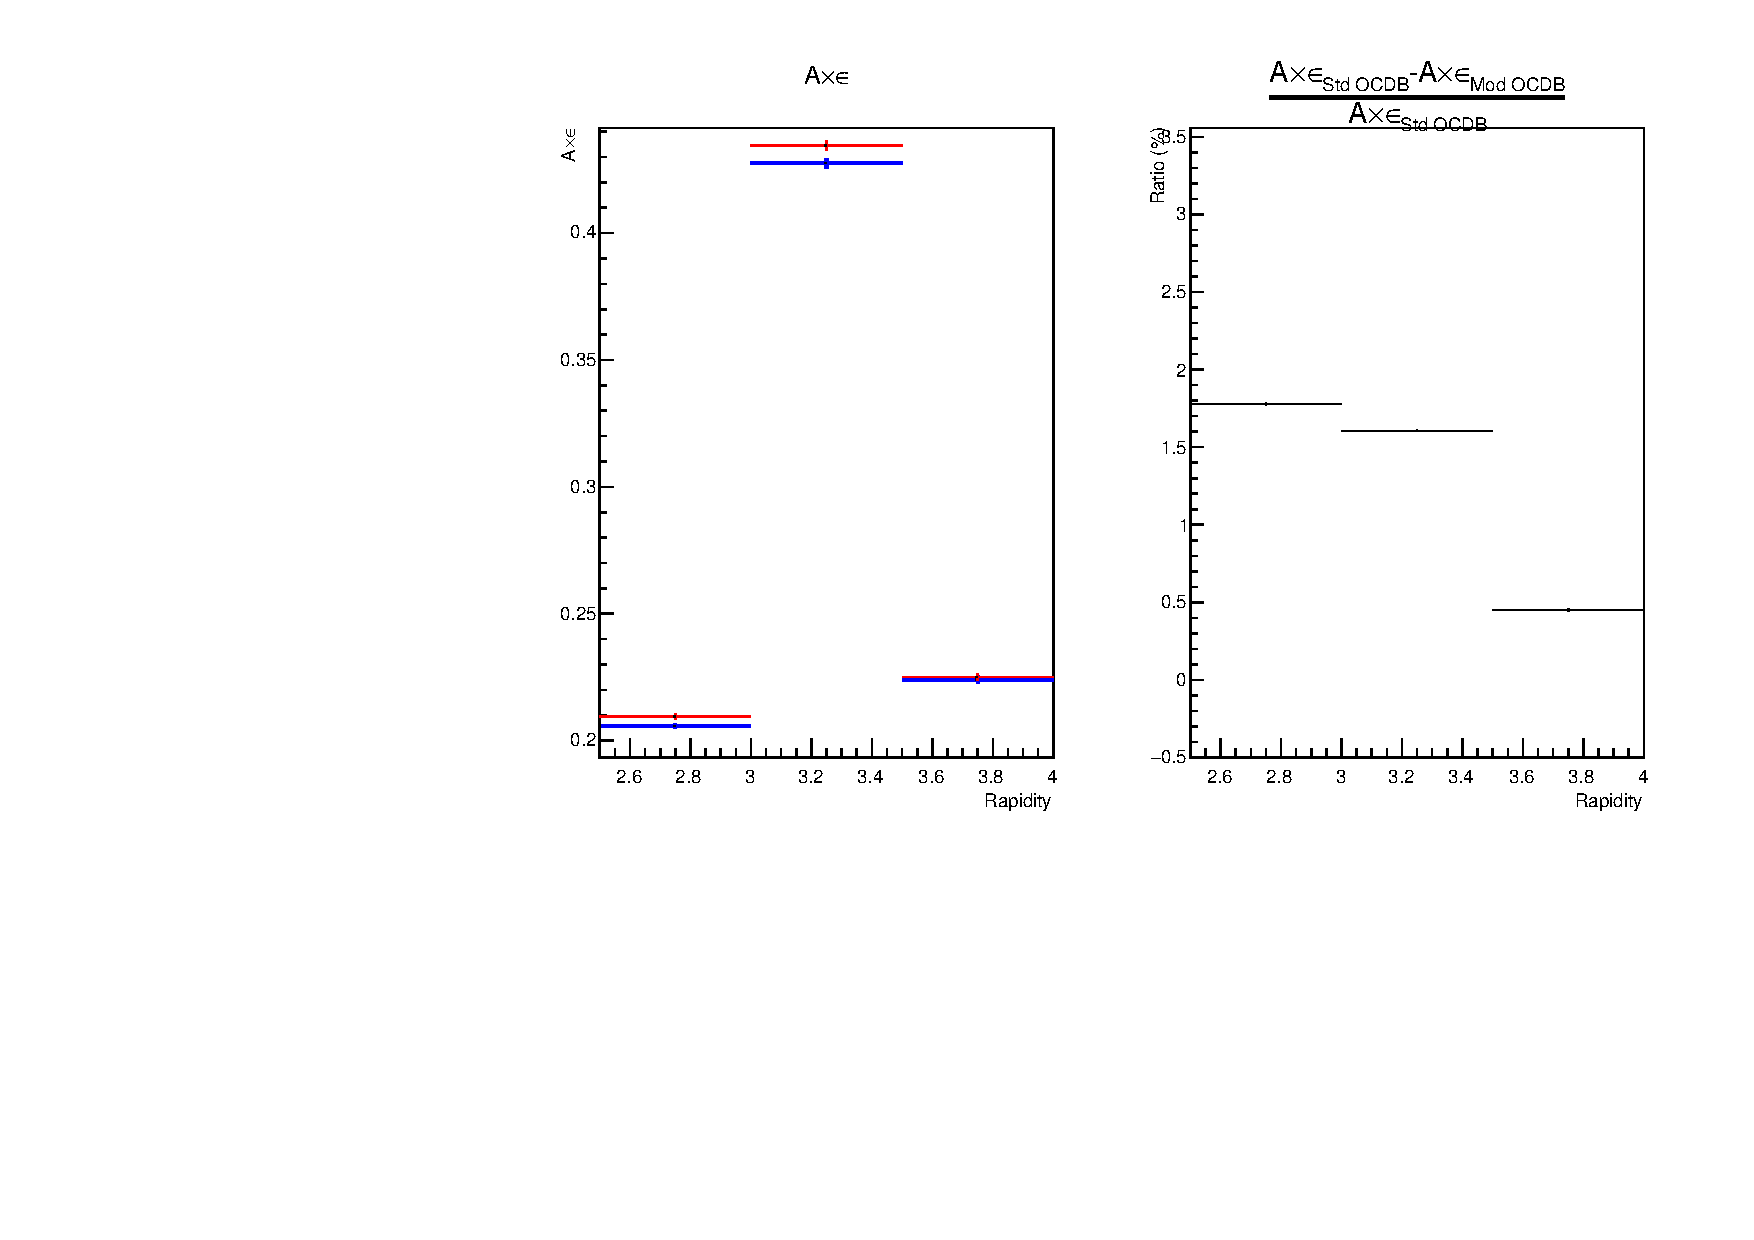
\includegraphics[width=0.45\linewidth]{Chapters/Analysis/Figs/AxEffSystError_NOCUT.pdf}
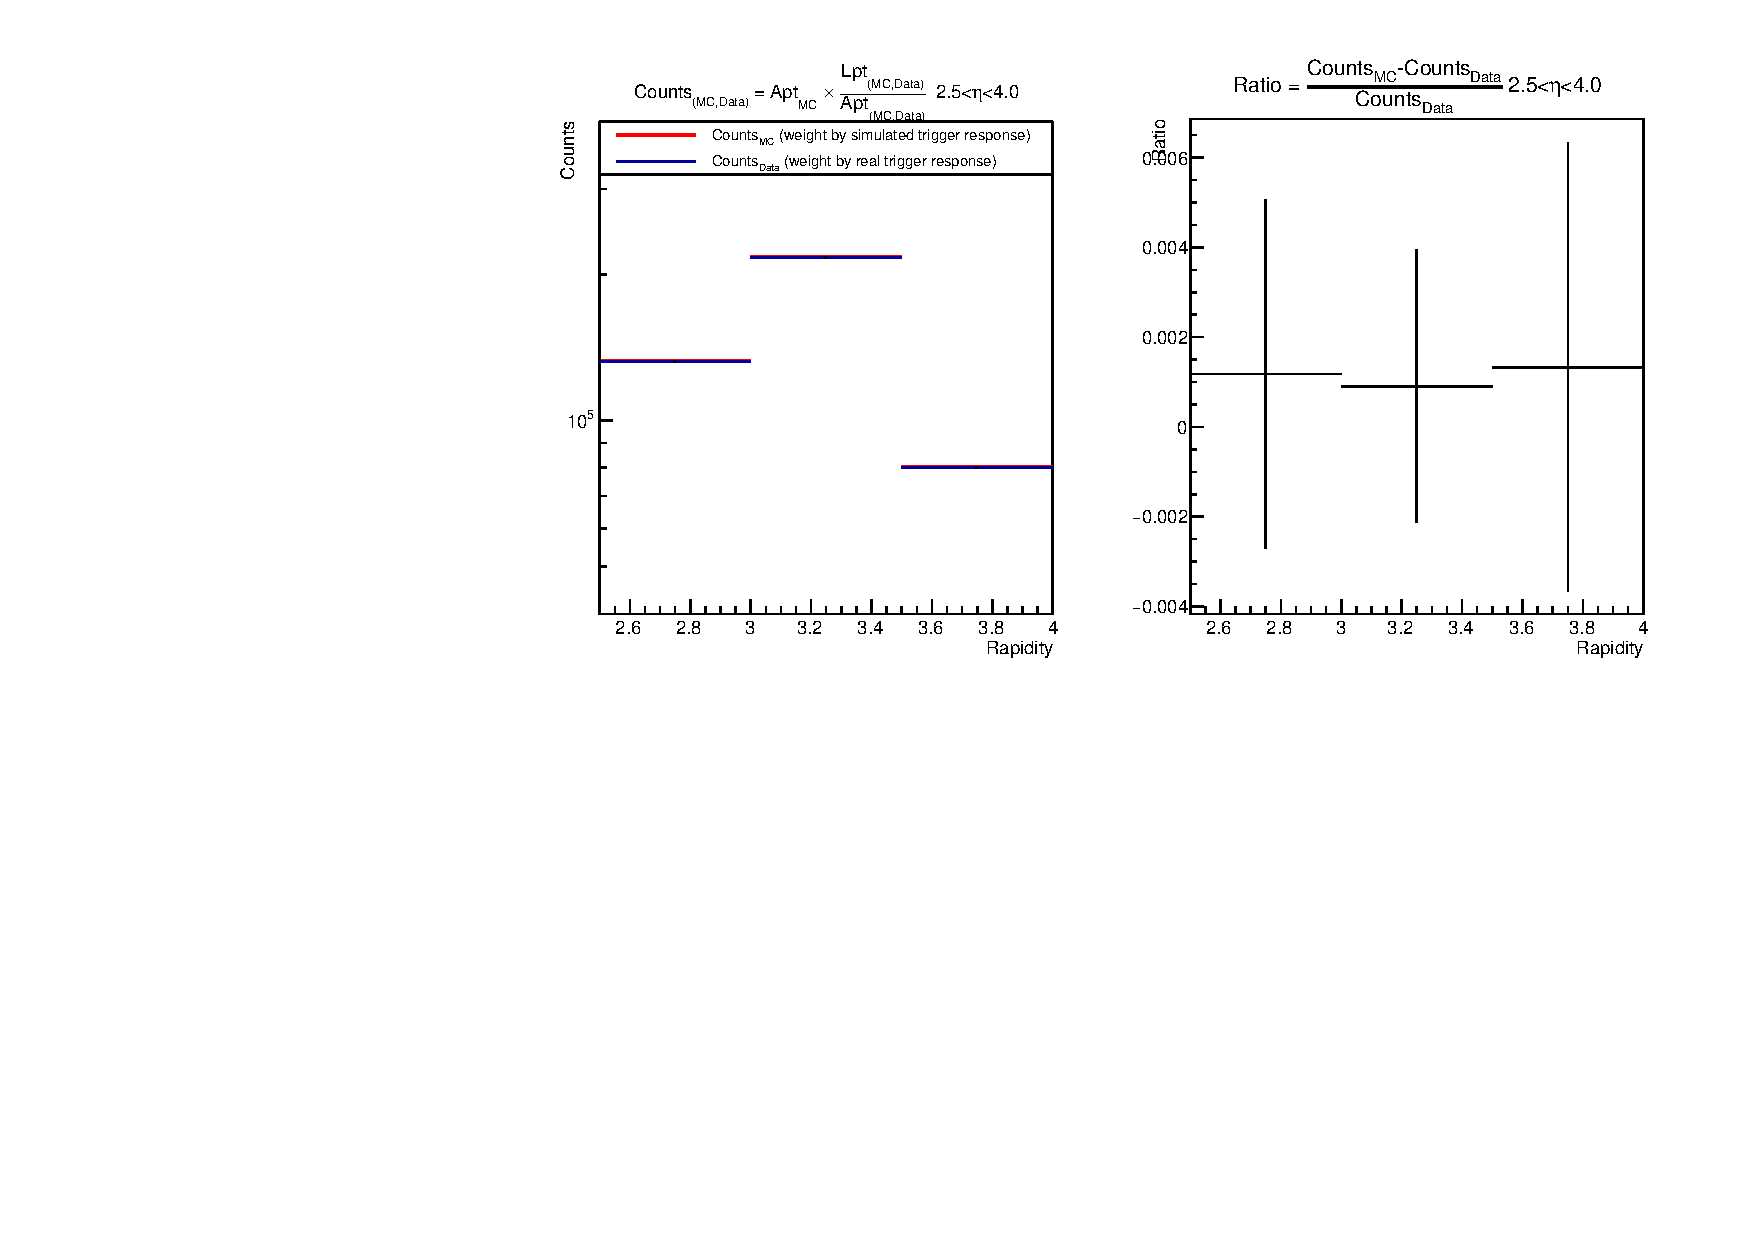
\includegraphics[width=0.9\linewidth]{Chapters/Analysis/Figs/ResponseFunctionSyst.pdf}
\caption{On left panel the muon trigger response function as a function of $y$ is shown. Trigger response is reweighted using Monte Carlo data (red) or real data (blue). Right panel shows the ratio of the two series as a function of $y$.}
\label{fig:trigsystRF}
\end{center}
\end{figure}

\begin{figure}[!htb]
\begin{center}
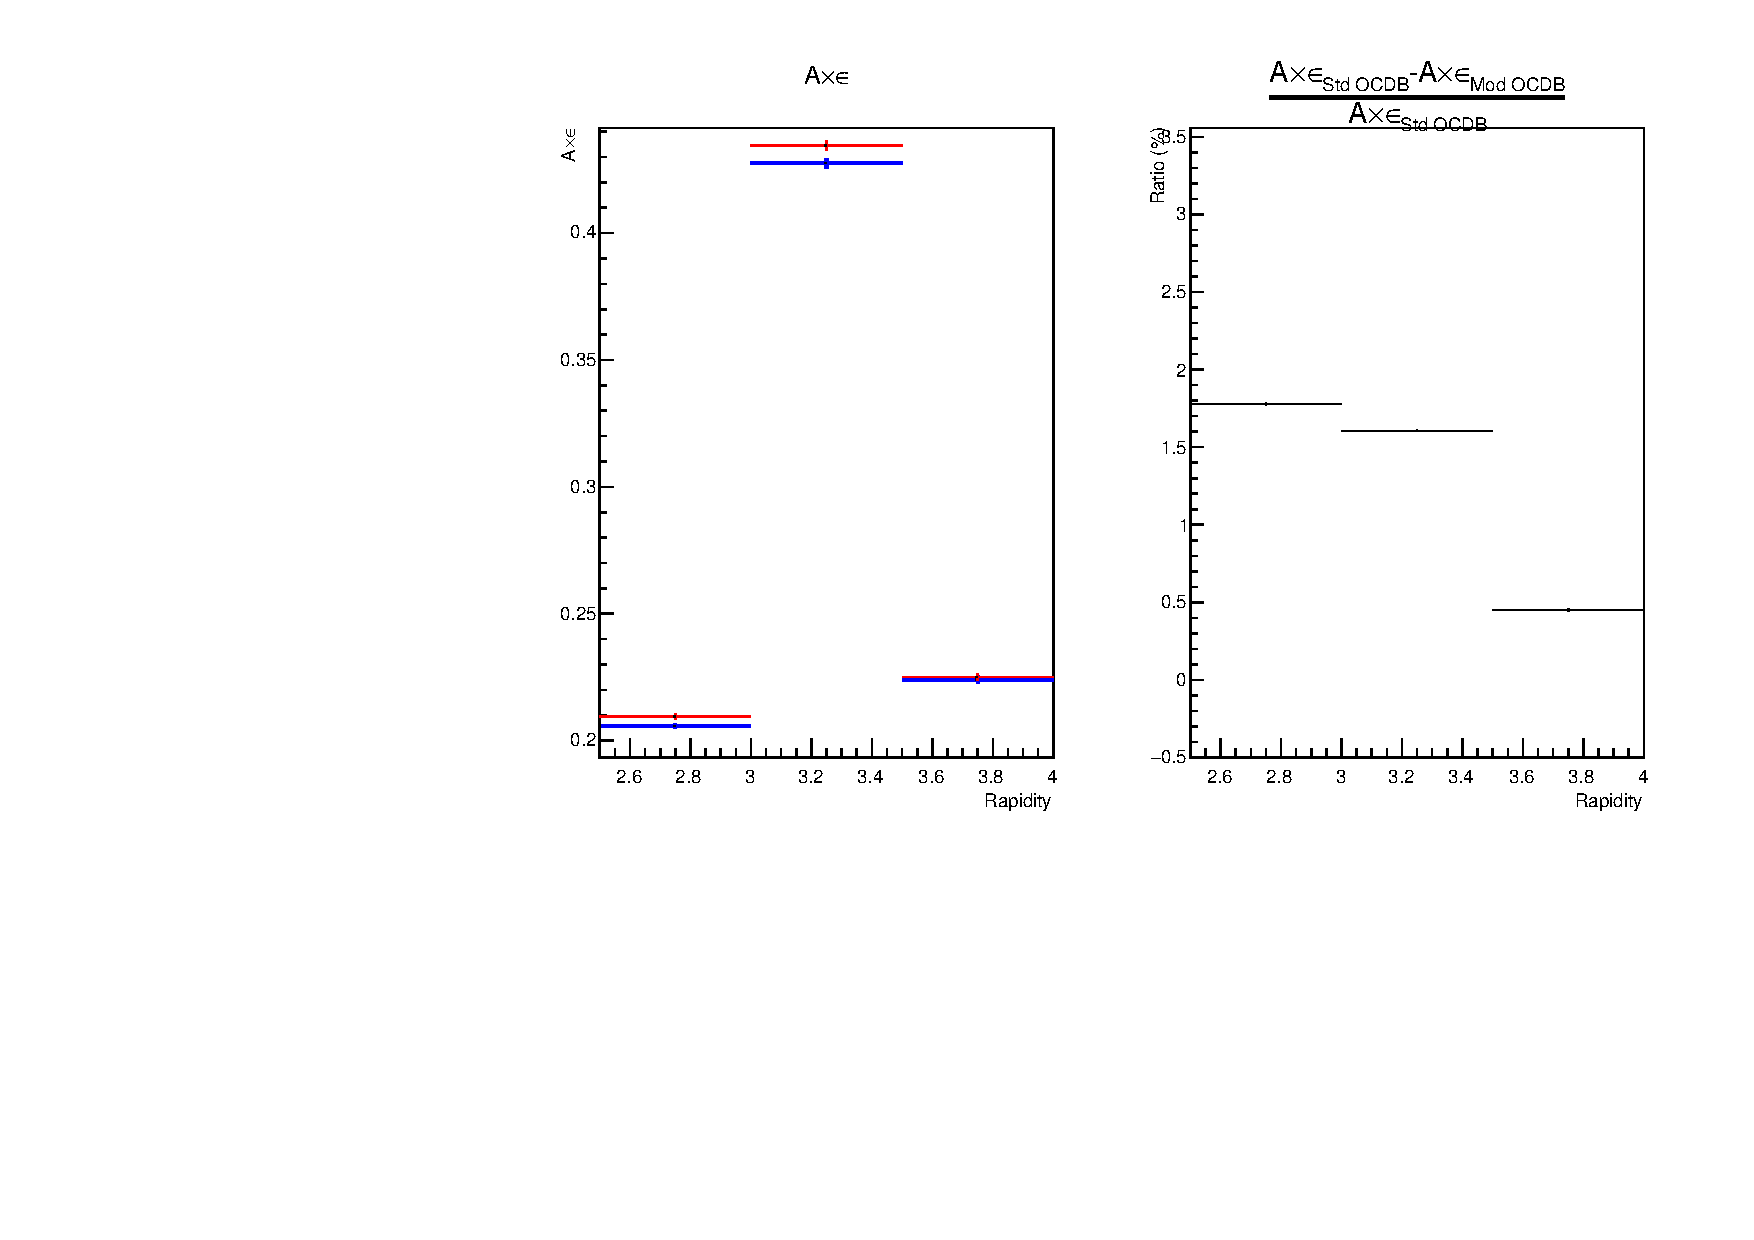
\includegraphics[width=0.9\linewidth]{Chapters/Analysis/Figs/AxEffSystError_NOCUT.pdf}
\caption{On left panel the muon trigger $A\times\epsilon$ as a function of $y$ is shown. Trigger efficiency is evaluated as the standard Monte Carlo set (red) or the real one (blue). Right panel shows the ratio of the two series as a function of $y$.}
\label{fig:trigsystAxe}
\end{center}
\end{figure}

The systematic uncertainty on the tracking efficiency is obtained starting from an evaluation of the single muon tracking efficiency in MC and data. 
This evaluation is performed via a procedure, detailed in ~\cite{Adam:2015isa}, based on the redundancy of the tracking chamber information.
The \upsi reconstruction efficiency is then obtained by combining the single muon efficiencies of the two systems, namely muon trigger and muon tracker.
The systematic uncertainty generated by the \upsi reconstruction efficiency is taken as the relative difference of the values obtained with the procedure based on MC and data.

The muon tracks for data analysis are chosen based on a selection on the $\chi^2$ of the matching between a track segment in the trigger system with the extrapolation of a track in the tracking chambers. 
The matching systematics is obtained by varying the $\chi^2$ selection cut in data and MC and comparing the effects on the track reconstruction efficiency~\cite{Adam:2016rdg}.

The systematic uncertainty on the centrality measurement is evaluated by varying by $\pm0.5\%$ the V0 signal amplitude corresponding to $90\%$ of the hadronic cross section in \pbpb collisions.
This choice is driven by the fact that the $90\%$ bin is used as anchor point to define the centrality classes.

The systematic uncertainty on the evaluation of $\sigma^{\rm pp}_{\Upsilon}$ is detailed in section \ref{sec:ppxsection}.

Finally, the systematic uncertainty evaluation of $F_{\rm{norm}}$ and $\langle T_{\rm{AA}}\rangle$ are described in~\cite{Adam:2016rdg} and~\cite{Abelev:2013qoq}, respectively.

The different systematic uncertainty sources on the $\raa$ calculation are summarized in Table~\ref{tab:syst}.
The correlated systematic uncertainties as a function of centrality, $y$ or $p_{\rm{t}}$ are indicated as type I. The uncorrelated ones as type II.
% In the table systematic uncertainties are correlated with the change of centrality, $\pt$ or $y$, are quoted as correlated (type I), otherwise they are treated as uncorrelated (type II).  

\begin{table}[!t]
\centering
\resizebox{1\textwidth}{!}{
\begin{tabular}{|c|c|c|c|c|c|}
\hline
\multirow{2}{*}{sources} & \multicolumn{4}{c|}{$\upsis$} & $\upsiss$ \\
\cline{2-5}
& Centrality & $y$ & $\pt$ & Integrated & Integrated \\
\hline
Signal extraction                               		& 4.3-6.1\%(II)                   	& 4.2-6.8\%(II)                  	& 5.2-8.7\%(II)                	& 4.1\%  	& 21.7\%\\
Muon \pt cut                               		& 0.3-2.4\%(II)                   	& 0.1-1.2\%(II)                  	& 0.1-2.4\%(II)                	& 0.7\%  	& 0.7\%\\
Input MC                                        		& 0.9\%(I)                       		& 0.6-2.6\%(II)                   & 1-1.4\%(II)                	& 0.9\%  	& 0.9\%\\
Tracker efficiency                             		& 3\%(I) and 0-1\%(II)      		& 1\%(I) and 3\%(II)		& 1\%(I) and 3\%(II)   	& 3\%  	& 3\%\\
Trigger efficiency                                       	& 3\%(I)                        		& 1.4-3.7\%(II)                   & 0.4-2.6\%(II)                 	& 3\%  	& 3\%\\
Matching efficiency                                     & 1\%(I)                        		& 1\%(II)                     	& 1\%(II)	                  	& 1\%  	& 1\%\\
%Centrality                                      		& 0.2-2.4\%(II)                     	& 0\%(I)                      	& 0\%(I)	                   	& 0\%  	& 0\%\\
Centrality                                      		& 0.2-2.4\%(II)                     	& -                      		& -	                   		& -  		& - \\
$F_{\rm{norm}}$                               		& 0.5\%(I)                        		& 0.5\%(I)                     	& 0.5\%(I)	                  	& 0.5\%  	& 0.5\%\\
$\langle T_{\rm{AA}}\rangle$                  	& 3.1-5.3\%(II)                      	& 3.2\%(I)                     	& 3.2\%(I)	                   	& 3.2\% 	& 3.2\%\\
${\rm BR}_{\Upsilon \rightarrow \mu^{+} \mu^{-}} \cdot \sigma^{\rm pp}_{\Upsilon}$                 	& 6.3\%(I)		                        	& 6.6-11.3\%(II)                 	& 5.5-11.5\%(II)		        	& 6.3\% 	& 7.5\%\\
\hline
\end{tabular}
}
\caption{\label{tab:syst}Summary of the systematic uncertainties for $\raa$ calculation. Type I (II) refers to correlated (uncorrelated) systematic uncertainties.}
\end{table}

%%%%%%%%%%%%%%%%%%
%%%%% DONE! %%%%%%
%%%%%%%%%%%%%%%%%%

%%%%%%%%%%%%%%%%%%%%%%%%%%%%%%%%%%%%%%%%%%%%%%%%
\section{Results}\label{section:results}

The nuclear modification factors for  inclusive $\upsis$ and $\upsiss$ production in \pbpb collisions at $\snn=5.02$ \rm{TeV} with $p_{\rm T} < 15$ GeV/$c$, $2.5 < y < 4$ and the 0--90\% centrality class are $R_{\rm{AA}}^{\Upsilon(\rm1S)}=0.37\pm0.02\text{(stat)}\pm0.03\text{(syst)}$  and $R_{\rm{AA}}^{\Upsilon(\rm2S)}=0.10\pm{0.04}\text{(stat)}\pm{0.02}\text{(syst)}$, respectively.
The quantities entering the \raa for the \upsiss have been determined exactly in the same ways as those for the \upsis.
The measurements show a strong suppression for both bottomonium states.

The value of the systematic uncertainties affecting the $R_{\rm{AA}}$ is comparable to those of the statistical ones.
To reduce the contribution of systematic uncertainties the ratio of the two $R_{\rm{AA}}$ can be computed.
% Since the decay kinematics of \upsis and \upsiss states are very similar, most of the systematic uncertainty sources entering the ratio cancel out.
However the dominant contributions to the systematic uncertainties, namely those related to signal extraction and the $pp$ cross section, are not simplified by the computation of the ratio.
The integrated ratio $R_{\rm{AA}}^{\Upsilon(\rm2S)}/R_{\rm{AA}}^{\Upsilon(\rm1S)}$ is $0.28\pm0.12\text{(stat)}\pm0.06\text{(syst)}$. 
An indication of a stronger suppression for \upsiss around $2.5\sigma$ is present.

A comparison between \upsis nuclear modification factor values at different energies might highlight a suppression dependence on the center of mass energy of the colliding system.
The ratio between the \upsis $\raa$ at $\snn=5.02$ \rm{TeV} and $2.76$ \rm{TeV} is $1.23\pm0.21\text{(stat)}\pm0.19\text{(syst)}$. 
The sources of systematic uncertainties entering the calculation of the ratio are considered uncorrelated, except for the \taa component, whose uncertainty cancels out. 
The ratio is compatible with unity within uncertainties, hence no energy dependence is observed within the present uncertainties.

%The centrality, $p_{\rm T}$- and $y$-dependences of the $\upsis \raa$ at forward rapidity at $\snn=5.02$ \rm{TeV} are shown in Fig.\ref{fig:raa_data} together with the published results by CMS at mid-rapidity at the same center-of-mass energy \cite{CMS:2017ucd}. 
The centrality, $p_{\rm T}$ and $y$-dependences of the $\upsis$ $\raa$ at forward rapidity at $\snn=5.02$ \rm{TeV} are shown in figure \ref{fig:raa_data}. 
A decrease of $\raa$ with increasing centrality is observed down to $R_{\rm{AA}}^{\Upsilon(\rm1S)}=0.33\pm0.03\text{(stat)}\pm0.03\text{(syst)}$  for the 0--10\% most central collisions.
The $p_{\rm T}$-dependence is observed to be compatible within uncertainties with a flat behaviour up to $p_{\rm T}=15$ GeV/$c$.
The $y$-dependence shows a $\raa$ compatible within uncertainties with a flat distribution, as already observed in the measurements at $\snn=2.76$ \rm{TeV} \cite{Abelev:2014nua}.
Since the uncertainties size further data is needed in order to have a stronger conclusion on the rapidity dependence of the $\raa$.

\begin{figure}[!t]
\begin{center}
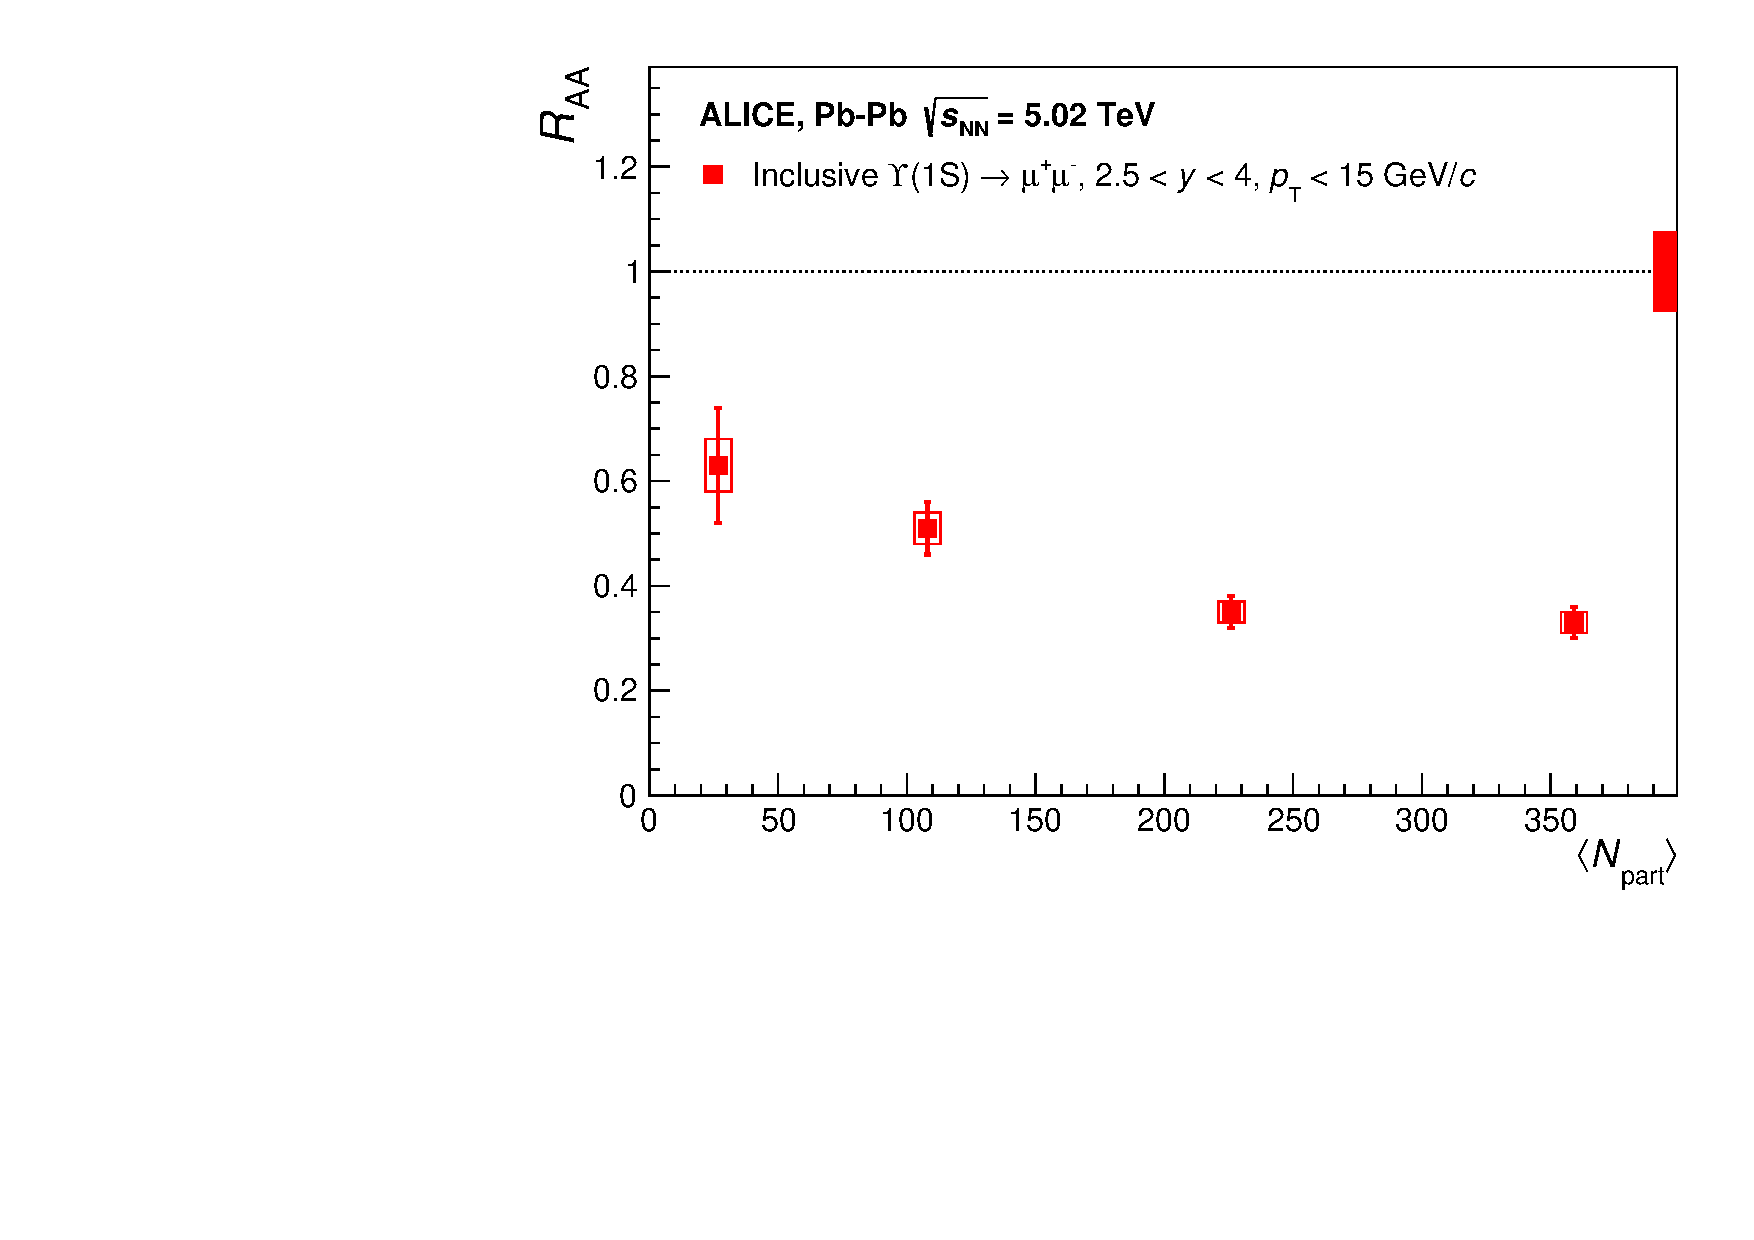
\includegraphics[width=0.9\linewidth]{Chapters/Analysis/Figs/RAA_Cent_ALICE2015.pdf} \\ 
%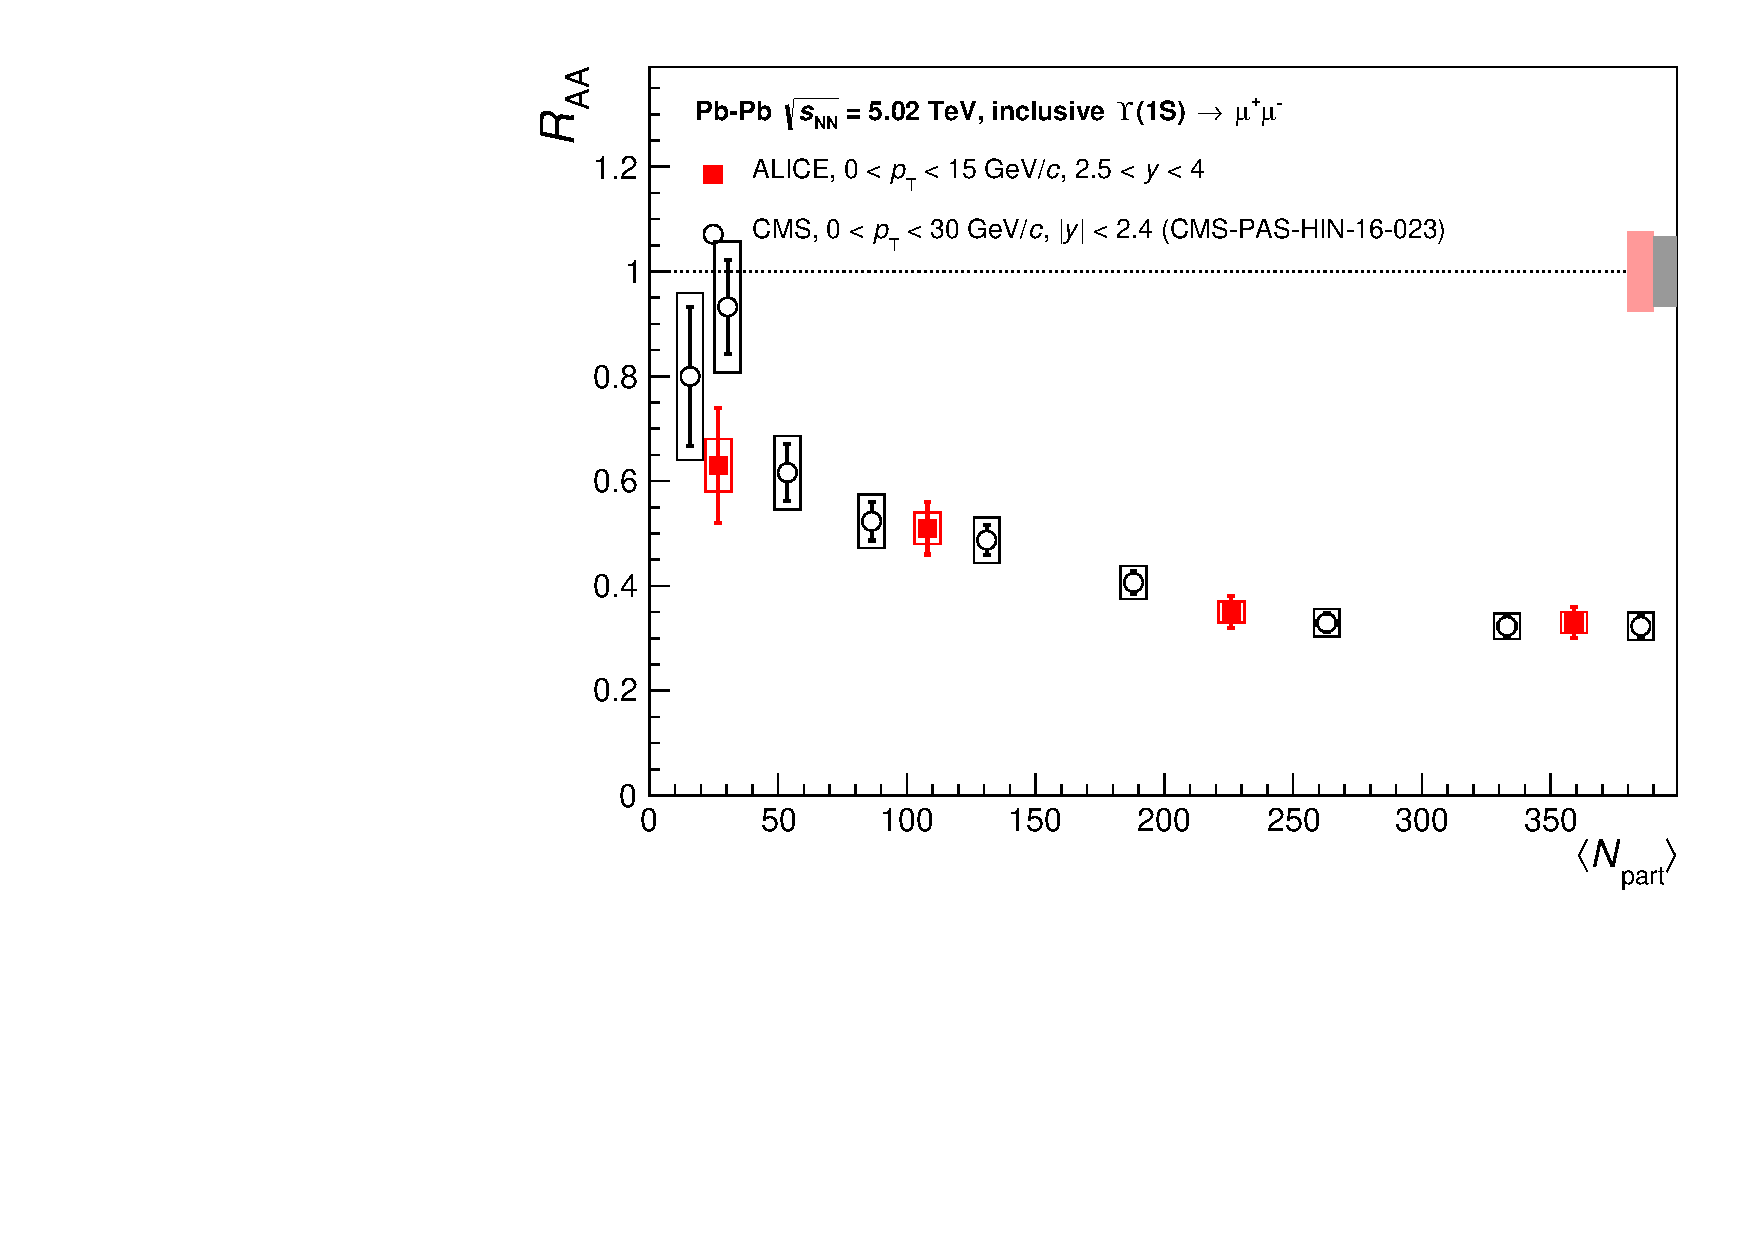
\includegraphics[width=0.5\linewidth]{RAA_Cent_ALICE2015vsCMS2015.pdf} \\ 
\end{center}
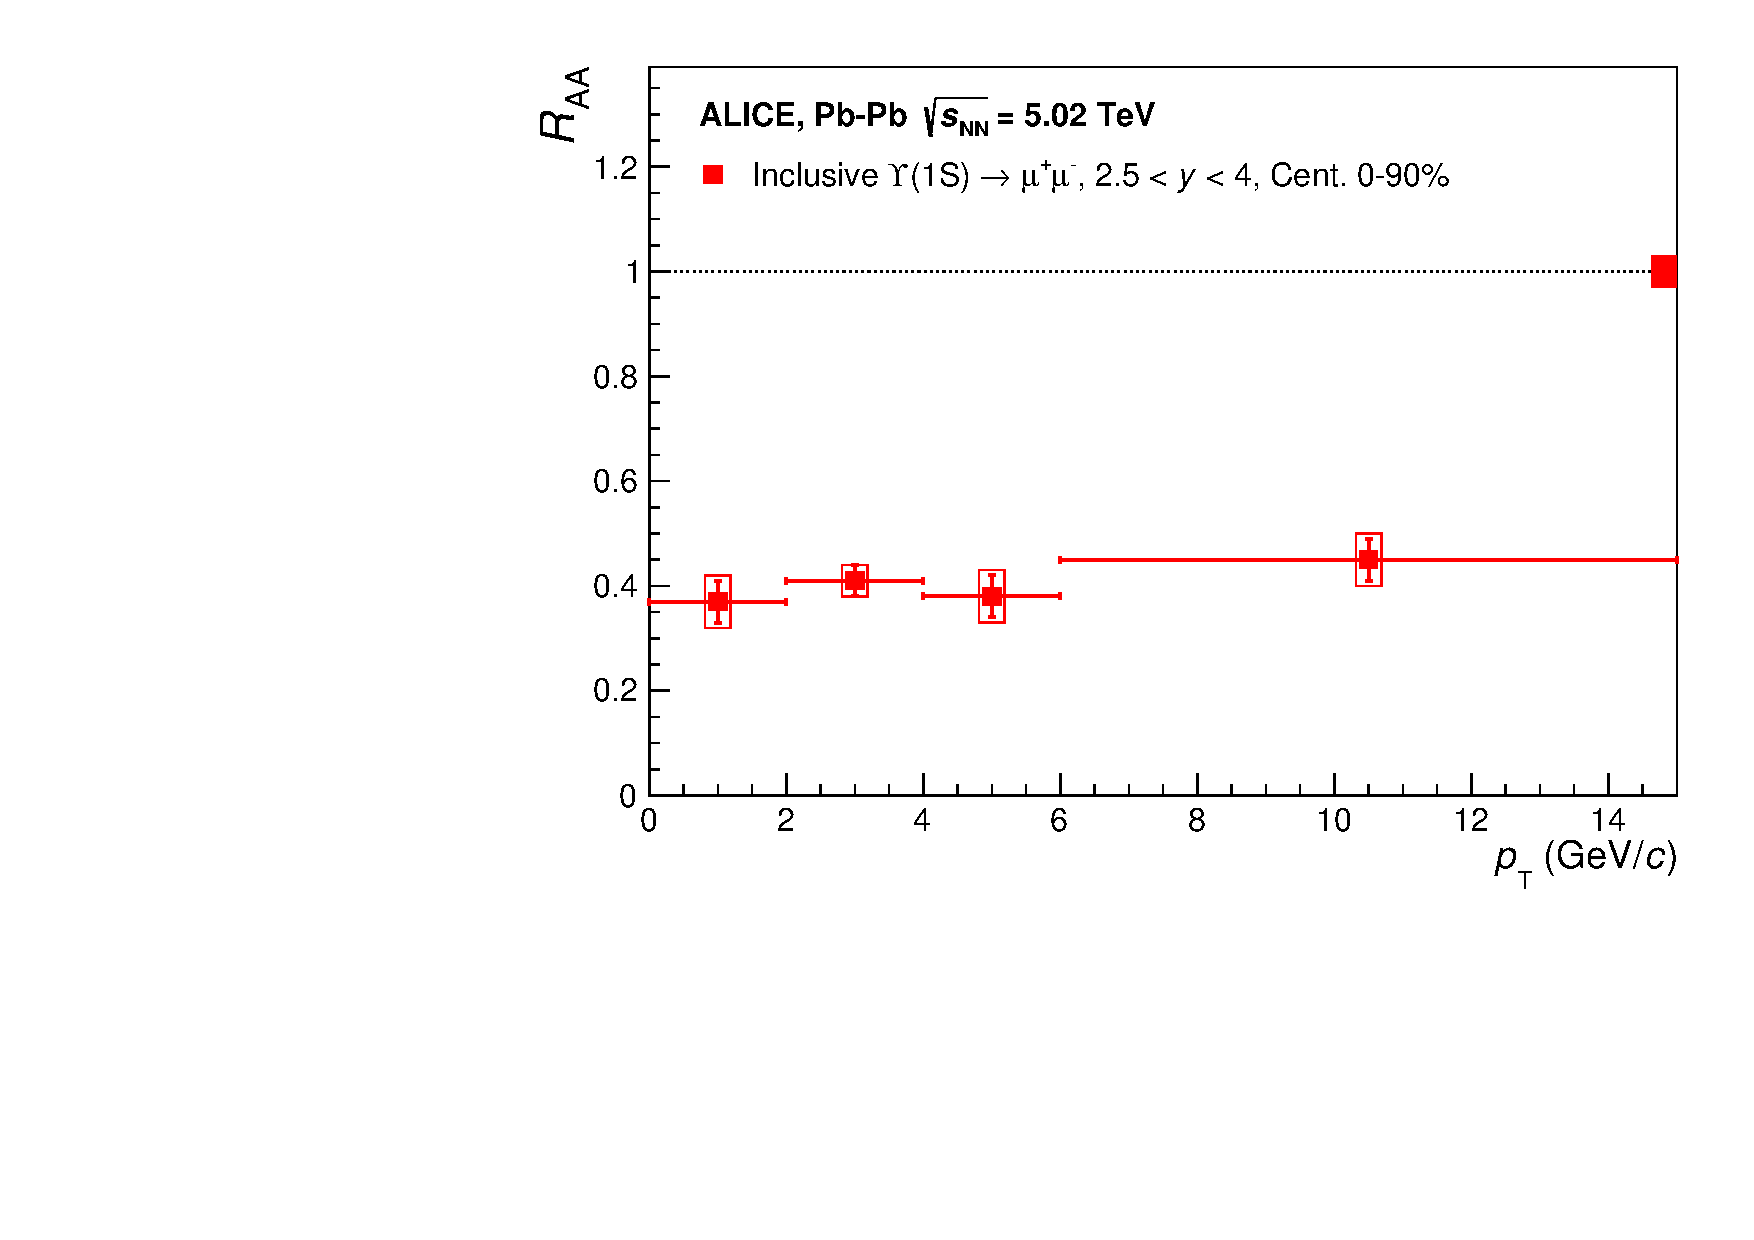
\includegraphics[width=0.5\linewidth]{Chapters/Analysis/Figs/RAA_Pt_ALICE2015.pdf}
\includegraphics[width=0.5\linewidth]{Chapters/Analysis/Figs/RAA_Y_ALICE2015.pdf}
%\includegraphics[width=0.5\linewidth]{RAA_Pt_ALICE2015vsCMS2015.pdf}
%\includegraphics[width=0.5\linewidth]{RAA_Y_ALICE2015vsCMS2015.pdf}
\caption{Inclusive $\upsis$ $\raa$ as a function of centrality (top), $\pt$ (left) and $y$ (right) at forward rapidity at $\snn=5.02$ \rm{TeV}. The vertical error bars and the boxes represent the statistical and uncorrelated systematic uncertainties, respectively. The relative correlated uncertainty is shown as boxes at unity.}
%\caption{Inclusive $\upsis$ $\raa$ as a function of centrality (top), $\pt$ (left) and $y$ (right) at forward rapidity (full red squares) at $\snn=5.02$ \rm{TeV} together with the CMS results at mid-rapidity (open black circles). The vertical error bars and the boxes represent the statistical and uncorrelated systematic uncertainties, respectively. The relative correlated uncertainties are shown as a box at unity.}
\label{fig:raa_data}
\end{figure}

The inclusive $\upsis$ $\raa$ measurements are compared to several theoretical predictions in Fig. \ref{fig:raa_models}.
The set of models used for comparison is composed by two transport models (TM1 and TM2)\cite{Du:2017qkv,Zhou:2014hwa} and one hydro-dynamical model \cite{Krouppa:2017jlg}.
While transport models follow the propagation of the free quarks in the medium, the hydro-dynamical models approach the QGP as a macro state.
Transport models use a rate-equation approach which accounts for both suppression and (re)generatio mechanisms in the QGP.
In hydro-dynamical models, the macro state "decays" in micro states ($e.g$ quarkonium states, open heavy flavor hadrons) at the freeze-out.

In the model quoted as TM1 \cite{Du:2017qkv}, the evolution of the thermal medium is based on a thermal-fireball expansion.
The feed-down contribution is taken into account based on measurements from ALICE and LHCb \cite{Abelev:2014qha,Aaij:2014caa,Aaij:2014hla}.
TM1 predictions are shown as bands, obtained varying the magnitude of nuclear shadowing effects, as described in ~\cite{Tuchin:2010pv}. 
The upper limit shown in Fig.~\ref{fig:raa_models} corresponds to the extreme case of the absence of shadowing while the lower limit reflects a reduction of $30\%$ due to shadowing.

TM2 \cite{Zhou:2014hwa} uses a 2+1 dimensional version of ideal hydrodynamic equations.
The uncertainties on these predictions are given by the spread caused by two sets of feed-down fractions to \upsis ground state:
\begin{itemize}
\item $27\%$ from $\chi_{\rm b}$; $11\%$ from $\Upsilon({\rm 2S}+{\rm 3S})$
\item $37\%$ from $\chi_{\rm b}$; $12\%$ from $\Upsilon({\rm 2S}+{\rm 3S})$
\end{itemize}
In TM2, the shadowing parameterization is based on EKS98 \cite{Eskola:1998df}.

Finally, the \upsis production cross section in $pp$ collisions at $\sqrt{s}=5.02$ \rm{TeV} in the rapidity range $2.5 < y < 4$ is taken as $\text{d}\sigma^{\rm\Upsilon({\rm 1S})}_{\rm pp}/\text{d}y=28.8$~nb in TM1 and $\text{d}\sigma^{\rm\Upsilon({\rm 1S})}_{\rm pp}/\text{d}y=30$~nb in TM2.
Those values deviate by about $2 \sigma$ (TM1) and $1.4 \sigma$ (TM2) from the result obtained using the $pp$ interpolation method reported in the previous section.

In the hydro-dynamical model \cite{Krouppa:2017jlg}, a thermal suppression of the bottomonium states is calculated using a lattice QCD-vetted complex-potential approach through a description of the medium evolution based on the 3+1d anisotropic hydro-dynamical model.
 In this recent study, no significant variation of the $\raa$ has been observed with respect to the plasma shear viscosity-to-entropy density ratio ($4\pi\eta/s$) parameter of the hydro evolution. 
Therefore, it is set to $4\pi\eta/s$ = 2, which is consistent with particle spectra fits.
The uncertainties of the model come from the heavy-quark potential uncertainty that was estimated by including a $\pm 15\%$ variation of the Debye mass of the QCD medium.
The latter is tuned by a fit to the real-part of the lattice in-medium heavy-quark potential.
The uncertainty of the Debye mass of the heavy-quark potential implies $\sim15\%$ uncertainty on the expected bottomonium \raa. 
Furthermore, the predictions shown in figure \ref{fig:raa_models} are referring to the initial momentum-space anisotropy parameter $\xi_0=0$, which corresponds to a perfectly isotropic QGP at the starting point of the hydrodynamic evolution at $\tau_0=0.3$ fm/$c$.
Finally, this model accounts for feed-down contributions but it includes neither a regeneration mechanism nor CNM effects. 

The centrality dependence of the $\upsis$ $\raa$ is fairly reproduced by the model calculations, as shown in the top panel of Fig.~\ref{fig:raa_models}.
The data is best described by TM1 when regeneration is included and by TM2 when regeneration is not taken into account.
The uncertainties on the measured point do not allow for a discrimination between the two models, hence a firm conclusion on whether the regeneration is present or not is not possible. 
The hydro-dynamical model describes the trend of the data, even if the measurements systematically lie on the upper edge of the uncertainty band for $\npart>70$.
This can be interpreted as a hint of a weaker Debye mass and thus a larger heavy-quark potential.

As a function of \pt (bottom left panel of Fig.~\ref{fig:raa_models}), the data favor the regeneration scenario of the TM1 model.
As for the centrality dependence, the hydro-dynamical model is in agreement with measurements even if the data points are systematically at the top edge of the uncertainty band.

For what concerns the $y$-dependence of the $\upsis$ $\raa$ only the hydro-dynamical model provides an estimation of the expected trend.
Even if the data points are compatible within uncertainties with the model estimation and with a flat distribution, some tension can be observed between the model-suggested trend and the trend shown by measurements (bottom right panel of Fig.~\ref{fig:raa_models}).

\begin{figure}[!t]
\begin{center}
\includegraphics[width=0.5\linewidth]{Chapters/Analysis/Figs/RAA_Cent_ALICE2015_Rapp_Zhou_Strickland_style3.pdf} \\
\end{center}
\includegraphics[width=0.5\linewidth]{Chapters/Analysis/Figs/RAA_Pt_ALICE2015_Rapp_Strickland_style3.pdf}
\includegraphics[width=0.5\linewidth]{Chapters/Analysis/Figs/RAA_Y_ALICE2015_Strickland_style3.pdf}
\caption{Inclusive $\upsis$ $\raa$ compared to predictions from two transport models \cite{Du:2017qkv,Zhou:2014hwa} and one hydro-dynamical model \cite{Krouppa:2017jlg} as a function of centrality (top), $\pt$ (left) and $y$ (right). See text for details on the models. While all models provide centrality dependence predictions, some of them do not provide $p_{\mathrm{T}}$ and/or $y$ estimations. The plots report all the available information at the moment of writing.}
\label{fig:raa_models}
\end{figure}

%%%%%%%%%%%%%%%%%%%%%%%%%%%%%%%%%%%%%%%%%%%%%%%%
\section{Summary}

The nuclear modification factors of inclusive \upsis and \upsiss production was measured with the ALICE detector at forward rapidity ($2.5<y<4.0$) and for $p_{\rm T}<15$ GeV/$c$ in \pbpb collisions at $\sqrt{s_{_{\rm NN}}}=5.02$~\rm{TeV}.

% The computation of double ratios between \upsis and \upsiss $\raa$ at $\sqrt{s_{_{\rm NN}}}=5.02$~\rm{TeV} and between \upsis $\raa$ at $\sqrt{s_{_{\rm NN}}}=2.76$~\rm{TeV} and $\sqrt{s_{_{\rm NN}}}=5.02$~\rm{TeV}.
The double ratio of the \upsis and \upsiss \raa was computed as well. 
The observed value of $ 0.28 \pm 0.12(stat.) \pm 0.06(syst.)$ is compatible with the hypothesis of a larger suppression for the higher-energy (more weakly bound) states.

Finally, the double ratio of the \upsi \raa measured in Pb-Pb collisions at $\sqrt{s_{_{\rm NN}}}=5.02$ and $2.76$~\rm{TeV} was computed as well. 
The result shows no significant energy dependence at the LHC.

% The ratio between \upsis and \upsiss productions is aligned  with the hypothesis of a binding-energy dependent sequential suppression, given the higher energy state is clearly more suppressed than the fundamental one.
% The ratio computed for \upsis at different energies, however, showed no significant energy hierarchy at the LHC energies.
% Even if no clear hint on an energy dependence of the suppression/recombination mechanisms at the LHC energies is present, from the comparison between ALICE results at the LHC and previous results at RHIC a symmetry between $J/\psi$ at RHIC and \upsis at the LHC can be noticed.
% This observation can suggest that a recombination mechanism similar to the one observed for $J/\psi$ at RHIC can be present for \upsis at the LHC.
% That can eventually be in agreement with the estimation of the average number of produced $c-\bar{c}$ and $b-\bar{b}$ pairs at the two accelerators energies.

The results have been compared with transport and hydrodynamic models.
The transport models are able to provide prediction with and without including recombination effects.
Comparing the measurements with the different predictions lead to no clear conclusion on whether recombination effects play a role has been possible yet.
Further measurements with larger statistics will be needed to improve the precision and to better constrain the models.
\chapter{Measurement and monitoring of Muon Trigger System performances}

\section{The RPC ancestors}
Before the invention of the RPCs, the typical ionization gaseous detectors were spark and streamer chambers.

\begin{figure}[!t]
\begin{center}
\includegraphics[width=0.95\linewidth]{Chapters/Performance/Figs/spark-chambers.pdf}
\caption{Spark chamber schematic with some details on the external trigger system and coincidence electronics.Extracted from \cite{wenzel:1966}}
\label{fig:SparkChamber}
\end{center}
\end{figure}

Spark chambers (fig \ref{fig:SparkChamber}) are detectors composed of a stack of metal plates put in a sealed box filled with an opportune gaseous mixture \cite{wenzel:1966}.
The metal plates are kept at high voltage, with an electrical field of at least $70 kV/cm$.
An ionizing particle which travels through the detector causes the ionization of the gas, which happens accordingly to a streamer development in which the primary electrons avalanche develops in $(10^{-8}÷10^{-7})s$ and then the secondary ionization and the streamer development happens in $(10^{-10}÷10^{-9})s$ \cite{wenzel:1966}.
This ionization is typically invisible, but, if enough voltage is applied to the plates, it can cause the drift of the ionized gas which can cause a trail of sparks revealing the ionizing particle path.
The application of the high voltage cannot be permanent, because in this case the creation of a electric arcs would lead to discharge of the whole system.
For this reason an additional detector is needed in order to trigger the application of the high voltage to the plates right during the passing of the ionizing particle.
Typically the high voltage trigger detectors are scintillators or photo tubes. 
In addition whenever a ionizing event happens, the whole interested plates get discharged due to the local conductivity change of the gaseous mixture.
After a full discharge the recovery time is macroscopic, around $10ms$, due the capacitor-like behavior of the plates stack.
In addition another disadvantage was clear: only particles crossing two electrodes caused a spark.

The high dead time due to electrical recovery and the need of an external HV trigger of the spark chambers caused the development of another kind of gaseous detector.
In the past the model for spark growth has prompted several groups \cite{chicovani:1964} to investigate the possibilities of arresting the discharge before the streamers have developed into a spark channel.
The most important consequence of this work is that the isotropic streamer chamber has been invented, in which particle trajectories at all angles to the applied electric field may be recorded.
In addition the streamer chamber allowed for the recording of more than $30$ tracks at a time.
In this case the electric field is not strong enough to cause an electric arc between the electrodes, but the gradient of the electric field stays strong enough to cause visible streamers around the particle path.
While the HV was still externally triggered by fast detectors, the much lower energy required to develop streamers allowed to reduce the pulse width to down to $60÷100ns$.
The typical way of recording a streamer chamber event was by a visible light photo of the streamer cavity.
For this reason the cavity walls required to be transparent.
The streamer mode helped in this task: while the sparks need to reach the electrodes to form, the streamer can be operated with electrodes which are either integrated in the chamber glass walls or external to the glass box.

\begin{figure}[!t]
\begin{center}
\includegraphics[width=\linewidth]{Chapters/Performance/Figs/streamer.pdf}
\caption{Stages in the growth of a streamer: (a) creation of initial seed electron and positive ion; (b) rapid acceleration of the electrons results in the formation of an avalanche; (c) growth of the avalanche until the internal field negates the applied field, and recombination causes photons to be emitted which produce more ion pairs; (d) the electrons released at head and tail of the initial avalanche grow into avalanches; (e) continuation of process with merger of avalanches and growth of streamer. From \cite{evans:1969}}
\label{fig:Streamer}
\end{center}
\end{figure}

For the first time the electric field was induced on the gas gap externally, making the gaseous mixture able to generate streamers upon ionization.
Further development of this technology, aimed at reducing the HV pulse length and height, eventually incurred in the avalanche operational mode.
While the streamer is a structure of avalanches which come to saturation and cause a subsequent set of new avalanches, a simple avalanche is a single drop of ionized gas which develops following the electric field gradient.
At CERN by applying a $300kV$ pulse of $5ns$ length to a gap of $lOcm$, they have been able to arrest the avalanches before growth into streamers.
By the way it was obvious that the discharge is reduced from spark mode to streamer mode to avalanche mode.
For this reason the light output diminishes and hence the optical problems become more severe.
At that point the limits of the optical readout (e.g. with a camera) started appearing and caused a further development of such detectors.

\begin{figure}[!t]
\begin{center}
\includegraphics[width=0.8\linewidth]{Chapters/Performance/Figs/RPCside.png}
\caption{Schematic representation of an RPC structure from the side.}
\label{fig:RPCside}
\end{center}
\end{figure}

The Resistive Plates Chamber (RPC) detectors were developed taking and improving the best know how achieved for both spark and streamer chambers.
The RPCs are composed of a thin gas gap of some millimeters of thickness and some planar resistive electrodes which serve as providers of the required electric field.
While the previous detectors were optically read, the RPCs were since the beginning intended to be read using external readout electrodes.
In the form of pads or crossing strips these metallic electrodes were intended to read the streamer or avalanche drift via the current induced on them by the ions and electron drift inside the gas gap.
The revolutionary idea behind RPCs consists in the use of resistive electrodes to provide the electric field.
By doing so, in fact, the discharge due to the local conductivity change of the gaseous mixture cause an equally local reduction of the electric potential between the electrodes, without causing a complete discharge of the whole system.
This aspect of the RPCs working mode allowed to drop the requirements for an external array of detectors which served as a trigger for the HV pulse, since the HV could be provided constantly and dynamically re-established in the case of a local discharge.
This development of the gaseous detectors technology brought back this approach on providing big coverage and cheap detectors capable of sustaining high particle rates providing fast response time ($ns$) with good spatial resolution (millimeter) and high efficiency.
RPCs are currently adopted, mainly as muon detectors, by ALICE, CMS and ATLAS at the LHC and many other particle physics experiments around the world.

\section{RPC's morphology and physiology}
RPC detectors are made of several layers of different materials.
First of all the gas gap is the innermost part of the detector and contains a gas mixture which will be discussed later.
The gas gap is surrounded by the high resistivity electrodes which are the HV providers and thanks to the high resistivity are able to spatially limit the discharge.
The roughness of the electrodes must be as low as possible to limit the peak discharge around surface anisotropies.


\begin{figure}[!t]
\begin{center}
\includegraphics[width=0.47\linewidth]{Chapters/Performance/Figs/oil_irradiation.png}
\includegraphics[width=0.47\linewidth]{Chapters/Performance/Figs/oil_no_irradiation.png}
\caption{Current trend over time for single side oil coated and double oil coated RPCs. From \cite{aliceRPC:2004}.}
\label{fig:RPCoil}
\end{center}
\end{figure}

For this reason the resistive electrodes are frequently coated with oils in order to improve the smoothness of the inner surface and to preserve the resistivity \ref{fig:RPCoil}.
Right outside the resistive electrodes an insulation layer made of plastic material is provided, in order to electrically decouple the internal electrodes and the readout ones.
The readout pads or strips are installed outside the insulation layer.
The edge of the chamber is sealed by means of plastic material walls and pipes for the flow of the gaseous mixture are installed along the edge.

The gaseous mixture of an avalanche RPC is not standard and each implementation can differ from any other one.
Even if differences are possible, several roles can be highlighted for the gases included in any specific formula:
\begin{itemize}
\item Donor gas: is the gas which should be ionized by the ionizing particle and whose constituents take part in the charge drift;
\item X-ray quencher: is a gas which has an high cross section for x-rays and high energy photons. This is needed in order to absorb recombination photons which can cause a degeneration in streamer;
\item Charge quencher: is a gas which provides high electro-negativity in order to limit the transversal development of the avalanche and reduce the probability of a streamer degeneration.
\end{itemize}

Several aspects of an RPC electric behavior enter the definition of an RPC working point.
First of all the working point is defined as the high voltage at which the chamber can provide enough detection efficiency for a specific application.
Typically this voltage is detected by performing an efficiency versus voltage scan of a specific RPC, and might differ from one RPC to another.
Apart the detection efficiency, other aspects are important and should be considered when selecting the working point of an RPC.
A dependence between the supplied HV and the distribution of the cluster sizes (namely the number of adjacent strips fired by a single particle) has been observed, hence while the efficiency arises when raising the HV, the spatial resolution might be affected.
Another aspect related to the HV value is the signal amplitude and the total charge deposed in the gas gap by a ionizing particle.

The readout of the chamber is performed via a front end electronics which is connected to the readout electrodes.
The readout sensitivity has to be tuned based on the signal amplitude of the chamber.
At this point two roads are possible.
A signal multiplication has to be performed in order to make detectable the ionizing particle.
The multiplication can be either performed by saturating the avalanche inside the gas gap, using the ionization process, or by keeping a low avalanche saturation in the gas gap, using an amplified electronics as readout.
In the second case the high voltage can be lowered with respect to the first case, in which the amplification in the gas gap in fed by the HV supply.

\section{The ALICE muon trigger RPCs}
The ALICE muon trigger system is made of four layers (MT11, MT12, MT21 and MT22) arranged in two stations spaced of $1.2m$, as shown in figure \ref{fig:ALICEmuon}.
Each layer is logically divided in two sides, inside LHC ring and outside LHC ring, or, in brief, inside and outside.
Each of the four layers is composed of 18 RPCs.
The chambers of the first two stations are slightly smaller than the ones of the third and fourth in order to cover the same rapidity range.
Three shapes of RPC are installed and correspond to long, short and cut shapes.
The short and cut shapes are intended to leave the necessary clearance for the beam line crossing.
The muon trigger RPCs are made of $6mm$ wide gas gaps with bakelite resistive electrodes and polyammide insulation layers.
The readout strips are copper made and their pitch can vary between three values: $1cm$, $2cm$ or $4cm$.
All the RPCs are equipped with one set of readout strips per side.
The strips of each side of the RPCs are reciprocally orthogonal.
The vertical (horizontal) strips, providing $x$ ($y$) hits, are called non-bending (bending) in relation to the dipole action on charged particles paths.
The currently installed front-end electronics is called ADULT and is not amplified.
71 RPCs are equipped with this electronics, while one RPC is equipped with a prototype of the FEERIC electronics which provides an integrated amplification stage.
The working point of the ADULT ALICE RPCs is $10200V$, while the FEERIC equipped RPC requires as much as $10000V$ to operate correctly.

\begin{figure}[!t]
\begin{center}
\includegraphics[width=\linewidth]{Chapters/Performance/Figs/ALICEmuon.png}
\caption{Grayed out ALICE with highlighted muon chambers and muon trigger chambers.}
\label{fig:ALICEmuon}
\end{center}
\end{figure}

Muon trigger RPCs have been deeply characterized in 2003 and 2004 at the CERN Gamma Irradiation Facility (GIF) installed at SPS.
A deep report on the outcome of such tests can be found in \cite{arnaldi:2004}.
Since the first GIF tests the results showed that while the streamer operation mode was satisfying for the $Pb--Pb$ collision rates, providing good spatial resolution and fast enough recovery, it wasn't the best option for proton-proton operation mode.
In fact in this case, considering a foreseen irradiation rate of $50 Hz\cdot~cm^2$ the integrated irradiation over the detectors lifetime would easily pass the limit of $100 Mhits\cdot~cm^2$.
The R\&D carried out by CMS and ATLAS have shown that operation in avalanche mode results in a higher detector lifetime compared to the streamer mode.
Even if the ADULT front end has been developed specifically for streamer operation mode, not providing an amplification stage and a dual threshold ($10mV$ and $80mV$ in streamer), the modification of the electronic thresholds allowed for the operation of the chambers and the electronics in an "highly saturated avalanche mode" or maxi avalanche (both threshold to $10mV$).
Following this tests the ALICE muon trigger RPCs operated in this mode since the beginning of the ALICE operations.
The working point, selected following those studies, was set at $10200V$ in standard atmospheric conditions ($T_0=293K$ at $P_0=1013.25mbar$).
During the operation of the chambers in the cavern, the provided voltage is dynamically adjusted taking into account the temperature and pressure values.
The HV tuning formula is reported in \ref{eq:HVcorrection}, where $HV_{nom}$ is the working point quoted above.

\begin{equation}
\label{eq:HVcorrection}
HV_{eff} = HV_{nom}\cdot \frac{T}{T_0} \cdot \frac{P_0}{P}
\end{equation}

This correction formula is able to keep at a constant level the effective voltage inside the gas gap.
In fact pressure and temperature variations might modify the chambers efficiency.
The studies reported in \cite{arnaldi:2004} evaluated the efficiency plateau position and width.
The operating voltage of $10200V$ in standard conditions was chosen as a voltage value setting the efficiency level above $90\%$ and higher than the plateau knee value, in order to allow the voltage to oscillate a bit without causing a massive modification of the efficiency.

The gaseous mixture used in the muon trigger RPCs has been tuned to avoid the formation of streamers and to improve the avalanche formation capabilities.
The mixture composition is as follows:
\begin{itemize}
\item 89.7\% Tetrafluoroethane ($C_2H_2F_4$)
\item 10.0\% iso-Buthane ($iC_4H_{10}$)
\item 0.3\% Sulfum esafluoride ($SF_6$)
\end{itemize}

\section{RPCs aging symptoms}
Likewise other gaseous detectors, the gas gap of the RPCs can degrade over time due to reversible and irreversible modifications of the performances.

Some causes of degradation, which can be mitigated by special measures, are related to the gaseous mixture.
For example the ALICE RPCs, and in general any other implementation of such detectors in modern experiments, are fed with a constant flux of gas in order to clean the gas from unwanted chemical compounds
I addition to the filtering of the gaseous mixture and the constant replacement of part of that, the gaseous mixture is humidified.
One of the risks for bakelite-made RPCs is the bending caused by the drying of bakelite layers.
The humidification of the gaseous mixture allows to constantly hydrate the inner surface of the bakelite electrodes, keeping the original gas gaps shape and avoiding changes of the bakelite resistivity \ref{fig:drywet}.

\begin{figure}[!t]
\begin{center}
\includegraphics[width=0.95\linewidth]{Chapters/Performance/Figs/dry_vs_wet.png}
\caption{Resistivity trend over time for prototype ALICE RPCs. In the top panel a chamber provided with dry gas mixture is shown, while in the bottom panel the gas mixture is humidified. Several marker styles correspond to several testing positions. From \cite{aliceRPC:2004}.}
\label{fig:drywet}
\end{center}
\end{figure}


The most important source of performance degradation is the amount of charge generated in the gas gap during irradiation at nominal voltage.
In fact the charge generated in the gas gap is deposed either on the resistive electrodes or can induce the generation of chemical compounds out of the gas mixture components.
These compounds might depose on the inner surfaces of the gas gap, creating peaks which can affect the chamber noisiness, as well as they can chemically attack the surfaces.
Both these situations can cause an increase of the noise rate of the chambers.
An high noise rate causes a local inefficiency of the detector due to the recovery time after a discharge.
Even if one would like to avoid as much as possible these irreversible alterations, they are physiological of the RPC detectors used in such high irradiation situations.
For this reason the monitoring of the chambers has to be performed in order to detect as soon as possible the most altered chambers and to proceed with their replacement with spare ones.
As found at the GIF tests the ALICE muon trigger RPCs are performing well enough at least up to a total deposed ionization charge of $50mC/cm^2$.
For the following studies this limit will be the theoretical limit at which any RPC should be replaced.

\section{MTR monitoring data sources}
The ALICE experiment is equipped with a complex safety and hardware monitoring system called Detector Control System (DCS).
This system is the interface which is usually used by the central operators and the detector's experts to perform action which modify the power supply, gas flow, cooling and electronics statuses of the detectors.
In addition to the interface role, the DCS is connected to a database which records the readings of all the sensors related to devices handled by the DCS.
For what concerns the MTR, the DCS is able to record each chamber current, voltage, gas flow , humidity and composition as well as other control parameters such as the external LV used to set the electronics threshold and the VME infrastructure working parameters.
The read out values are stored in a DCS database which can be accessed using custom Siemens WinCC applications in order to produce plots and trends for several variables over time.
The data points are saved in the DCS database following two guidelines.
First of all the lectures are stored in the database whenever a given threshold on percent variation, with respect to previously stored value, is passed.
Additionally a slow clock ($5$ minutes) triggers the storage of the current lecture, in order to keep track of smaller variations as well as of the stability of a given system.

\begin{figure}[!t]
\begin{center}
\includegraphics[width=0.7\linewidth]{Chapters/Performance/Figs/OCDB.png}
\caption{Cartoon representing the data flow of collision data, DCS data and software infrastructure informations. At the end of the run the Experiment Control System (ECS) sends the DIM trigger to the Shuttle, which is responsible of the migration of data in the GRID storage. The shuttle receives from the Data Acquisition System (DAQ), the Detector Control System (DCS) and the High Level Trigger (HLT) the information relative to the involved detectors. The data is packed together and moved to the GRID. From \cite{Zampolli:2010zz}.}
\label{fig:shuttle}
\end{center}
\end{figure}

The ALICE experiment status can be either data taking (when collecting physics data) or not.
In the first case a database, the Offline Conditions Data Base (OCDB), stores all the calibration and alignment data is stored.
A connection channel between the DCS infrastructure and the OCDB allows for the storage of the DCS readings during data taking.
This allows to keep a track of the working conditions of the detectors, of the LHC status, the beam condition, the magnets activity and any other important information.
The OCDB is not a database in the usual sense.
All the data collected by ALICE is stored on the storage elements of the computing GRID.
The files, in ROOT format, containing the stored data are not all stored in a single place.
The OCDB provides a layer of access to those files, despite their geographical distribution.
In order to provide this access flexibility, the OCDB uses some parameters stored as file meta-data.
One of these meta-data is a validity interval defined using run numbers.
It appears clear, at this point, that the OCDB structure strongly depends on the run numbers and that measurements performed outside of a data taking run cannot be stored in the OCDB.
Due to this peculiarity and design choice the OCDB allows for the storage of DCS reading only during data taking runs, in which at least some of the ALICE's detectors are being read out.


\section{MTR integrated charge measurements}
As already stated the ALICE muon trigger detectors aging strongly depends on the alteration caused by irradiation.
In particular the biggest part of the damages is not caused by the ionizing potential of the radiations and particles, but by the ionized gas particles inside the gas gap and their chemical action of the RPC surfaces.
Given the limit of $50mC/cm^2$, the maximum irradiation level at which the RPCs are guaranteed to work nominally, the evaluation of the total integrated charge is of crucial importance.
In particular the junction of an RPC sees a current flow which has three components \ref{eq:itot}:
\begin{itemize}
\item Ohmic component: the ohmic component of the current is due to the low conductivity of the gas gap and of the structure of the chamber. This part of the current depends linearly with the applied voltage, hence its name;
\item Environmental irradiation-caused: natural or activated radiation sources and cosmic rays might emit ionizing radiation and particles towards the chambers, causing an avalanche, hence a discharge;
\item Produce particle-caused: this current component originates by the crossing of ionizing particles produced during the LHC collision.
\end{itemize}

\begin{equation}
\label{eq:itot}
i_{tot}=i_{net}+i_{cosmic}+i_{env}+i_{ohm}
\end{equation}

The first two components of the total current are always present if the detector is kept at the nominal working voltage.
The third component of the current depends on the operations of the LHC and the collision luminosity.
From an aging point of view the ohmic current won't cause any permanent modification of the RPC, then it should not be taken into account in the computation.

A detector might be switched on and fully operational when no data taking is being performed, for example between one run and the following one or when no beam is provided by LHC and ALICE is taking cosmic data.
In this kind of situations the amount of current flowing trough the system corresponds to the sum of the ohmic contribution and the environmental one.
Measuring the amount of current flowing in a chamber in these conditions would provide a measurement of $i_{dark}$, defined in equation \ref{eq:idark}.

\begin{equation}
\label{eq:idark}
i_{dark}=i_{cosmic}+i_{env}+i_{ohm}
\end{equation}

The current that one should integrate in order to evaluate the aging of a chamber is the net current ($i_{net}$) corresponding to the current due to the formation of avalanches caused by particles produced during collisions.
Once $i_{dark}$ is measured, the evaluation of $i_{net}$ can be done subtracting it to $i_{tot}$ measurements.
The integration of $i_{net}$ over time will provide the aging index that can be compared to the limit value obtained in the tests.

This measurements are not possible using the OCDB as data source.
In fact the OCDB polls DCS readings and stores them permanently only when data taking is being performed.
Even if this condition can happen both with beam collisions and during cosmic runs, the coverage of the dark periods of the MTR is partial.

The work presented in this chapter was originated from the idea of combining OCDB and DCS measurements using the well established OCDB data retrieving interface and the AMANDA/DARMA DCS database (Archive DB in figure \ref{fig:shuttle}) access tool, in order to increase the working conditions coverage with respect of the OCDB-only approach.
In addition the granularity provided by the DCS is much better with respect to the on of the data propagated to the OCDB, but the DCS readings have no run number, beam condition or LHC status information.
By combining the two data sources a better understanding of the MTR performances would arise, giving the possibility to perform trend and distribution studies, as well as correlation studies between MTR parameters and external conditions such as collisions luminosity.

\section{MTR performance analysis framework}
As a subject of this thesis a brand new analysis framework for MTR performance analysis has been developed.
This framework's main task is to combine the data coming from OCDB and AMANDA/DARMA in order to create a complete set of data which can be used for specific studies of trends and correlations regarding the MTR system.
As an additional value to this project, the framework aims at providing a reliable tool which is accessible and open source.
Having a centralized repository, with the possibility of participating to the development of the framework and to the fixing of eventual software bugs, can improve both the user experience and the user base hence the bug detection capability.

The framework stands on a base class which is intended as a container of all the data relative to a particular run.
This class is called \code{RunObject} and contains the following information:
\begin{itemize}
\item Run number: identifies the current run;
\item Start and End of Run: or SOR and EOR. Are the timestamps defining the data taking inside a run;
\item Average HV: average value (weighted over time) of supplied HV. One value per each of the 72 RPCs;
\item Average $i_{tot}$: average value (weighted over time) of supplied current.  One value per each of the 72 RPCs;
\item Average $i_{dark}$: average value (weighted over time) of dark current, extrapolated via the algorithm.  One value per each of the 72 RPCs;
\item Integrated charge: integral of the $i_{net}$ over the run.  One value per each of the 72 RPCs;
\item Bending scalers: total number of hits on the bending side of the chamber.  One value per each of the 72 RPCs;
\item Not bending scalers: total number of hits on the bending side of the chamber.  One value per each of the 72 RPCs;
\end{itemize}

The framework is composed by two acting classes.
The first, \code{MTRShuttle}, is the one which performs the data retrieving, parsing and manipulation.
It is responsible of merging the data coming from the two sources and of creating a vector of \code{RunObject}s to store the data.
The second class is \code{MTRBooster} which elaborates the \code{RunObject}s vector created by \code{MTRShuttle} and presents to the user the possibility to generate trend and correlation plots using a friendly interface for the specification of the plot options.

The \code{RunObject} arrays are filled by a \code{MTRShuttle} instance using data coming from OCDB and DCS database.
Their filling is performed using a either a local or a remote copy of the OCDB and a local copy of the DCS database.
Several steps are performed by the filling algorithm.
They are listed right after:
\begin{enumerate}
\item DCS data points are parsed from two files containing $i_{tot}$ and $HV$ readings;
\item OCDB data regarding runs identified through a provided list of run numbers is parsed either from the GRID OCDB or a local copy. Beam conditions, HV readings and scalers values are stored;
\item Additional dummy runs are created, filling the periods between runs whose information is found on the OCDB;
\item Current readings are defined "dark" switching a \code{bool} flag using the OCDB information about beam presence. See schema in figure \ref{fig:iDarkFlag};
\item A linear interpolation of all the $i_{dark}$ values is performed. Each current reading has two floating point values corresponding to $i_{tot}$ and $i_{dark}$. For values flagged as dark the two values are equal. For all the others the value of $i_{dark}$ is set using the interpolation of dark current values. See schema in figure \ref{};
\item For each \code{RunObject} the average $i_{tot}$ and $i_{dark}$ values are computed via the weighted average of all the $i_{tot}$ and $i_{dark}$ falling between the SOR and the EOR;
\item For each run the integral over time of the $i_{net}$ values is performed and stored in the relative \code{RunObject}.
\end{enumerate}

\begin{figure}[!t]
\begin{center}
\includegraphics[width=0.7\linewidth]{Chapters/Performance/Figs/darkCurrentFlagging.pdf}
\caption{Cartoon representing the process of dark current readings flagging by combining OCDB and DCS data. The lines are represented on an arbitrary horizontal time axis. 
The first line represents the current readings stored in the DCS database. 
The frequency of those measurements is not fixed. 
The second line represents with boxes the duration of several runs. 
Gray boxes show physics runs, while the black box represents a run in nominal conditions without beam (cosmic run). 
The first line currents can be flagged either as $i_{tot}$ if within a non-cosmic run or as $i_{dark}$ otherwise. 
They are represented in the last two lines accordingly. }
\label{fig:iDarkFlag}
\end{center}
\end{figure}

\begin{figure}[!t]
\begin{center}
\includegraphics[width=0.7\linewidth]{Chapters/Performance/Figs/interpolation.pdf}
\caption{Cartoon representing the interpolation process.
The green and blue points represent $i_{tot}$ and $i_{dark}$ readings, according to figure \ref{fig:iDarkFlag}.
The dashed vertical lines represent the projection on the time-axis of $i_{tot}$ readings.
The solid line connecting $i_{dark}$ measurements represents the linear interpolation.
The crossings between the $i_{dark}$ interpolation curve and the vertical dashed lines, are the $i_{dark}$ values attributed to $i_{tot}$ measurements.
Such values are highlighted with red crosses.}
\label{fig:interpolation}
\end{center}
\end{figure}

Once the data parsing has been accomplished the plots can be created via an instance of \code{MTRBooster}.
Several methods are presented to the user in order to specify the plot one wants to create.
These methods are described in details here after:
\begin{itemize}
\item \code{SetPlane},\code{SetSide} and \code{SetRPC}: optional methods to request a plot specific for a given RPC. The default value causes all the RPCs to be plotted in different colors. For example calling \code{SetPlane} and not the other two methods causes the plot to show all the RPCs belonging to the selected MTR plane. Same goes for calling only \code{SetSide};
\item \code{SetX} and \code{SetY} are the mandatory methods which allow the user to select what \code{RunObject} data to use as $x$ and $y$ coordinate in the plot. Selecting one of the available timestamps as $x$ value produces a trend plotRange setters: methods to set the time frame in which the data have to be plotted are provided. A set of three methods (\code{SetRange(min,max)},\code{SetMin(min)} and \code{SetMax(max)} is provided for setting the range using timestamps, run numbers or human readable dates;
\item Run selections: methods to select standard types of runs are provided. One can easily plot only runs with nominal HV value, runs with beam presence, runs without beam, runs with nominal HV and no beam and runs adequate for the integrated charge computation;
\item \code{AccumulateY}: this method makes the plotter integrate the $y$ values while plotting. Since each run has the value of integrated charge within the run, this option is needed to provide the amount of integrated charge over the whole analyzed period;
\item \code{NormalizeToArea}: the $y$ values (and the $x$ ones if not a trend plot) are divided by the RPC area to provide a value over $cm^2$;
\item \code{PlotAverage}: superimposes to the generated plot the average behavior of the plotted RPCs;
\item \code{PlotMinMax}: superimposes to the generated plot the two plots of the RPCs whose last point is the highest and lowest of the plotted set of RPCs.
\end{itemize}

The framework has been extensively tested and the plots presented in the following sections of this thesis have been produced by means of the new framework, merging the two available data sources for the first time.

\section{Definition of dark current and dark rate and dark current interpolation procedure}
One crucial point is how to determine if a rate or a current reading are indeed "dark" readings.
First of all lets recap the definition of dark current and give the definition of dark rate.

The dark current is the measurement of current which physiologically flows trough the detector when it is supplied with working point HV and no collision-induced irradiation is present (e.g. when no beam is present in the LHC).
This current has an ohmic component and an irradiation one, the second caused by environmental radioactivity and cosmic rays reaching the detector.
The dark rate is the rate observed and measured in the same conditions, i.e. at nominal HV and when no collision in being performed.
This rate should be correlated with the natural radioactivity and cosmic rays incidence, but may contain a contribution related to unmasked noisy read-out channels.
In addition, since the dark rate is read-out by the electronics, dead channels might cause blind spot which in turn makes the rate to be lower than expected.

The dark runs can be defined in various ways.
Selecting runs taken with physics setup without beam presence (flagged as "COSMIC") are the safest choice, but this kind of runs is less frequent and provides less coverage of the operation period.
Selecting calibration runs allows to better cover the operation period, since at least two calibration runs are performed at the beginning and at the end of any physics run.
Measurements of dark current trends using cosmic or calibration runs only are displayed in figures \ref{fig::iDarkCOSMIC} and \ref{fig::iDarkCALIB}.
Assuming that the dark current should e constant without beam presence, one can observe a strange behavior for dark current computed using calibration runs only.
Some dark current variations which aren't completely understood are present.
For this reason this work uses only cosmic runs to estimate the dark current and dark rate values.

\begin{figure}[!t]
\begin{center}
\includegraphics[width=0.7\linewidth]{Chapters/Performance/Figs/iDarkCOSMIC.pdf}
\caption{Average dark current trend computed with the described procedure using cosmic runs only. Each point corresponds to a run. The $x$ value is obtained via the average of all the RPCs dark currents, while the $y$ value is the timestamp which corresponds to the end of run.
\label{fig:iDarkCOSMIC}
\end{center}
\end{figure}

\begin{figure}[!t]
\begin{center}
\includegraphics[width=0.7\linewidth]{Chapters/Performance/Figs/iDarkCALIB.pdf}
\caption{Average dark current trend computed with the described procedure using calibration runs only. Each point corresponds to a run. The $x$ value is obtained via the average of all the RPCs dark currents, while the $y$ value is the timestamp which corresponds to the end of run.
\label{fig:iDarkCALIB}
\end{center}
\end{figure}

At the moment of deciding which procedure to adopt to perform the dark current interpolation, in order to assign dark current values to non-dark current readings, two possibilities were spotted:
\begin{enumerate}
\item The interpolation is a moving linear fit performed on a group of $N$ dark current readings;
\item The interpolation is a linear interpolation of the two immediately surrounding dark current readings.
\end{enumerate}

While the first option is less sensible to overestimation caused by localized spikes, extending the set of currents to a fixed number $N$ of readings might make the algorithm take in account readings which are far in time with respect to the measurements for which the dark current value has to be set.
By doing so the risk of taking dark current readings extending over a time range in which non-recorded modifications of the detector state happened is high.
If, for example, the detector has been switched off for a while and switched on between the set of $N$ readings, some dark current readings will correctly represent the latest detector status, while the ones preceding the switch off will induce an overestimation of the dark current on the algorithm.
For these reasons, in order to limit the injection of artifacts by the algorithm, the second approach has been selected.
For the sake of completeness one should point out that the second option is equivalent to the first one in which $N=2$.
From an operative point of view this grant the additional advantage of avoiding a time consuming set of linear fits, replacing the minimization procedure with the analytic solution for a line segment crossing two points.

\section{Aging indicators}
As already stated previously, the CERN GIF tests of our RPCs have highlighted that a safe and satisfying performance level in granted up to an integrated charge of $50 mC/cm^2$.
The integrated charge is for this reason the main aging indicator for our RPCs.
If the integrated charge crosses the limit the chamber behavior might become unstable.
For this reason RPCs getting closer to the tests limit have to be replaced at the first possible occasion.

In addition to the evaluation of the integrated charge some others aging indicators can be spotted.
Even if the RPCs discharge is spatially limited by their resistivity, a localized discharge causes a temporary inefficiency due to the fact that the voltage should be reestablished.
The dark current is an interesting parameter, since it is usually related to the smoothness of the inner surfaces.
In fact having a coarse and spiked inner surface is not ideal: the irregularities might enhance the spikes effect, hence the frequency of dielectric breakdown.
This situation can lead to a local efficiency drop, more or less important depending on the ratio between the breakdown frequency and the HV recovery time.
In case of a worsening of the inner surfaces smoothness one might expect an increase over time of the dark current.

Another parameter, related to similar considerations, is the dark rate.
All the considerations performed for the dark current are valid also for the dark rate.

The three observables presented up to this point are studied trough the analysis of their values plotted over time.
Additional studies and observations may be performed using meaningful correlation plots.
Such plots, which are provided out of the box by the new MTR analysis framework, allow for the correlation of two of the stored variables.
For example the correlation plot between the net current and the rate observed at nominal HV during collisions can be fitted with a sloped line.
The angular parameter of the fit is an evaluation of the deposed charge per crossing ionizing particle.
A distribution of such parameter for the whole set of 72 RPCs might help spotting the outliers, namely the RPCs for which the charge deposed for a given ionizing particle is higher.
The detectors showing an higher charge per ionizing particle have to be strictly monitored, since their integrated charge will increase much stronger with respect to the normal ones.

The framework allows to produce distributions of the recorded values with respect to the beam conditions, hence relationships between the colliding systems and their energy and the RPCs behavior may be studied.

\section{Data selection}
The objective of this analysis was to perform a performance study of the ALICE muon trigger's RPCs throughout the whole operative life of the detectors, namely from 2010 to current days.
While the retrieval of DCS data for the whole period is trivial since the only possible selection is timestamp-based, the data downloaded from the OCDB can be selected using several flags.

In order to opportunely flag the DCS current readings either as dark or not it was needed to select runs with no beam and nominal HV supply.
After some tests the choice converged on the selection of the runs which on the ALICE electronic logbook are flagged as COSMICS.
In fact these runs are the only ones which guarantee the data taking was performed without collisions or beam presence and that the muon trigger was set at the nominal working HV.
Another run-kind candidate was the CALIBRATION type, which characterizes runs which are performed normally at the end of a data taking run in order to check the status of the front-end electronics.
Even if normally these runs are performed with the detector at nominal HV they are often repeated with the detector moved in safe position (i.e. around $8500V$) and/or some beam movements and modifications in the LHC.
The comparison of the new framework with and independent algorithm tested as right provided some checks: the selection of CALIBRATION runs was leading to a wrong estimation of the dark current, while using the COSMIC runs the two algorithms converged at the same results.
A total of around $5200$ cosmic runs have been used for this analysis.

The scalers values are not stored in the DCS database, hence it is necessary to download OCDB information for all the runs performed with beam presence and collisions in the LHC.
More than $12000$ runs have been selected, covering $pp$, $p-Pb$ and $Pb-p$, $Pb-Pb$ and $Xe-Xe$ colliding systems at all the center of mass energies provided by the LHC since the beginning of the operations.

\section{Performance analysis}
Several aging indicators for the 72 RPCs of the ALICE muon trigger will be presented and commented, trying to highlight eventual problematic RPCs which should be replaced.
A particular focus on the FEERIC-equipped RPC will address the main differences between the old and new read-out electronics from the chambers operations point of view.

\subsection{Dark current trend}
The evaluation of the dark current trend is fundamental to understand the health of the inner surfaces of the detectors.
This working parameter strongly depends on the presence of spikes on the boundary surfaces of the RPCs, hence can be used as a diagnosis tool.
In figure \ref{fig:iDark4Planes} a view of the trends of the dark current measurements as a function of time (date) is presented, each panel corresponds to the trends of the RPCs installed in MT11, MT12, MT22 and MT21 from top to bottom.
The dark current measurements are reported in $\mu~A/cm^2$, since dark current values have been divided by the corresponding RPC area.
Given the RPCs' areas are not all the same, this procedure helps to produce results which can be compared.

\begin{figure}[!t]
\begin{center}
\includegraphics[width=0.7\linewidth]{Chapters/Performance/Figs/iDark4Planes.pdf}
\caption{Dark current trends for each RPC over the whole operation period. The 72 trends are divided by plane (clockwise from top left MT11, MT12, MT22, MT21). For each plane the average plot is shown. Each point corresponds to a run. The $x$ value is obtained via the average over time of the dark current measurements, while the $y$ value is the timestamp which corresponds to the end of run.
\label{fig:iDark4Planes}
\end{center}
\end{figure}

A general view of the situation can be read from the trend of the black series of points, which corresponds to the average of all the RPCs reported in each panel.
The overall average trend presents a slight increase over 8 years of operation for all the four planes of the MTR.
This effect is imputable to two effects.
The first is the aging of the RPCs, as described in previous sections.
The second is the increase of the LHC luminosity over the years of operation, which causes the activation of materials which is reflected by the increase of dark current while no beam is present.

Sometimes a reduction of the dark current value can be observed.
This effect is more important and clearly noticeable at the beginning of each year.
It is commonly accepted that such a reduction of the dark current flow is caused by the yearly winter shutdown which undergoes for all the CERN LHC facilities.
In fact every year the beam operations are stopped for a winter period which typically lasts from late November to the first 3/4 months of the following year.
During this period the irradiation caused by the beam operations is absent.
At the same time the gas flow trough the chambers extracts impurities and eventually improves the inner surfaces smoothness.
This recovery time causes a reduction of the dark current and can systematically be observed for all the RPCs.

The overall status of the MTR RPCs appears to be good.
Comparing the specific trends of each RPC with the average trend one can easily observe than the increase of the average trend is mostly caused by some outliers.
In fact around 4/5 RPCs per plane, over a total of 18, present a dark current value strongly superior to the average trend.
This behavior indicates that most of the RPCs present a much more stable behavior.
The outliers of this trend can be considered the worst case scenario and should be monitored with attention in order to promptly notice eventual worsening of performances.

\subsection{Net current and integrated current trend}
This work presents for the first time a method to combine data from OCDB and DCS databases capable of subtracting the contribution of dark current from the evaluation of the integrated current.
In order to do so the net current should be evaluated starting from the total current and the dark current readings, through the procedure presented in the previous sections.

The net current measurements are reported in figure \ref{fig:iNet4Planes} as a function of time (date).
Each panel corresponds to the trends of the RPCs installed in MT11, MT12, MT22 and MT21 from top to bottom.
The net current measurement represents the current related merely to the irradiation of the detectors, hence it is expected to have a baseline at $0 \mu~C/cm^2$ and increases related to the beam presence and type.
The expected behavior is observed through the whole time range.

\begin{figure}[!t]
\begin{center}
\includegraphics[width=0.7\linewidth]{Chapters/Performance/Figs/iNet4Planes.pdf}
\caption{Net current trends for each RPC over the whole operation period. The 72 trends are divided by plane (clockwise from top left MT11, MT12, MT22, MT21). For each plane the average plot is shown. Each point corresponds to a run. The $x$ value is the difference between the average total and dark currents, while the $y$ value is the timestamp which corresponds to the end of run.
\label{fig:iNet4Planes}
\end{center}
\end{figure}

The net current plot has been integrated over time in order to obtain the integrated charge growth over time.
The results, sampled during the whole time range, are shown in figure \ref{fig:ICharge4Planes} where MT11, MT12, MT22 and MT21 are plotted (clockwise, from the top left panel).
The integrated charge trend shows various slopes, spanning from constant behavior during shutdowns of LHC to steep growth during the highest luminosity periods.
The already noticed recovery effect, observed after the shutdowns while studying the dark current trends, can be observed in the integrated charge trend as well.
After flat periods (i.e. periods with no irradiation of the chambers) the integrated charge growth starts slowly, increasing continuously.
The detectors response to various levels of irradiation is not linear and depends on their previous status.
This effect seems to suggest that the RPCs' behavior depends on how much time they have at disposal to recover after a high irradiation period, as if the net current had some sort of inertia.
Further monitoring and future specific tests might confirm such phenomenon.

\begin{figure}[!t]
\begin{center}
\includegraphics[width=0.7\linewidth]{Chapters/Performance/Figs/ICharge4Planes.pdf}
\caption{Integrated charge trends for each RPC over the whole operation period. The 72 trends are divided by plane (clockwise from top left MT11, MT12, MT22, MT21). For each plane the average plot is shown. Each point corresponds to a run. The $x$ value is the integral of net current since the beginning of the operations, while the $y$ value is the timestamp which corresponds to the end of run.
\label{fig:ICharge4Planes}
\end{center}
\end{figure}

The comparison between different RPCs within the same plane highlights that their response to irradiation is neither constant in time nor constant between different detectors.
Some detectors integrated charge overtakes on the one of other RPCs which present a much more stable behavior.
While some RPCs present an integrated charge which is systematically higher than that of the rest of the RPCs of the plane, but the trend of the plot seems aligned with that of others, other RPCs present sudden variations of the trend slope.
The RPCs which present sudden variations of the trend have to be monitored with attention as they might become the best candidates for a replacement.

It is worth mentioning that the new analysis framework allows to specify which RPCs have been replaced and when.
For this reason MT12 outside 6 presents an integrated charge reset to $0\mu~C/cm^2$ after the time-stamp at which it's been replaced. 

\subsection{Dark rate trend}
The dark rate trend is shown in figure \ref{fig:DarkRate4Planes}.
The informations which can be obtained from this set of graphs is complementary to that of dark current one.
Observing an increase of the dark rate is a clear symptom of aging.
In fact the dark rate is defined as the rate measured when no beam is present in the LHC.
The dark rate is then induced merely by environmental radioactive background or by spontaneous discharges in the gas gap.
For this reason, assuming the environmental background to be constant, any modification of the dark rate is induced by physical modifications of the inner surfaces or, in general, of the RPC health.

\begin{figure}[!t]
\begin{center}
\includegraphics[width=0.7\linewidth]{Chapters/Performance/Figs/DarkRate4Planes.pdf}
\caption{Dark rates trends for each RPC over the whole operation period. The 72 trends are divided by plane (clockwise from top left MT11, MT12, MT22, MT21). For each plane the average plot is shown. Each point corresponds to a run. The $x$ value is the average rate during a given cosmic run, while the $y$ value is the timestamp which corresponds to the end of run.
\label{fig:DarkRate4Planes}
\end{center}
\end{figure}

In reality a variation of the environmental background should be taken into account.
In fact right after the beam operations a radioactive activation of equipment close to the MTR and of the detector itself has been observed.
For this reason a temporary increase of the dark rate if foreseen, even if the beam is not present anymore.
The signature one should look for is not a temporary increase of the dark rate, but a not complete recovery of the dark rate back to the level measured before a period with beam presence.

Analyzing the trends one can observe that some RPCs show a growth of the dark rate over the whole period of operation.
An average of $4/5$ RPCs per plane show such trend and stand clearly over the average trend shown in black.
The chambers which show such behavior are the same which present and higher dark current with respect to the bulk of the RPCs.
Is worth mentioning that even if some outliers are detected most of the RPCs are still operating at the original level of dark rate after around 8 years of continuous operation.
In that sense the dark rate trend is a good cross-check of the symptoms already detected with the dark current studies and the integrated charge ones.
The affected RPCs have to be monitored to check their efficiency and to constantly ensure that their effectiveness as detectors is not being affected by the increase of the dark rate.

\subsection{Rate-net current correlations}
The possibility to study correlations of different parameters was introduced with the new analysis framework.
Using this new feature allows one to understand deeper the behavior of the RPCs.
The correlation plot which allows to better understand the health of a detector is the one representing net current values correlated with measured rate.

Looking to the correlation plot, the slope shown by the bulk of points relative to a given RPC is correlated to the charge deposed in the detector per each hit.
Fitting the correlation plot with a line can extract that value.
This derived measurement is interesting, since can easily highlight RPCs with abnormal discharge per hit.
Worth pointing out that this procedure won't highlight the presence of noisy channels which discharge easier, since such events would modify both terms of the ratio defining the slope of the graph.
One can observe that the bulk of measurements has a transversal size which is neither negligible nor compatible with a straight line.
Deviations leading to this spread are related to different energies of the crossing particle and various crossing angles of the particle.
A stronger (weaker) ionizing power and longer (shorter) path inside the gas gap work together to create deviations from the average behavior.

The correlation plot of net current and rate with beam presence is shown in figure \ref{fig:iNetvsRate4Planes}.
The behavior of the RPCs revealed by this correlation plot is aligned with previous measurements of other working parameters: while most of the chambers show a similar correlation between the two measurements, some of them clearly deviate from the bulk of points.
In order to have a smaller dead time after a hit (the time required to recover the local HV drop) the charge released per hit should be kept as low as possible.
A displacement the points to a zone representing lower charge deposed per hit is rarely (if not) expected, since the RPC health and status should worsen over time.
Points showing a displacement in this direction are rare and not grouped in clusters.
The absence of measurements clustering allows to suppose that the same causes of the bulk transversal spreading are responsible for these displacements.
Displacements towards the zone of the plot representing a higher charge per hit are instead typical, since the conductivity of the gas gap can increase over time.
In this case one can immediately note that such displaced points are grouped in clusters.
Since each point represents one of the analyzed runs, the fact that in various runs a given RPC has shown a recurring higher charge per hit gives more significance to the measurement.

\begin{figure}[!t]
\begin{center}
\includegraphics[width=0.7\linewidth]{Chapters/Performance/Figs/iNetvsRate4Planes.pdf}
\caption{Dark rates trends for each RPC over the whole operation period. The 72 trends are divided by plane (clockwise from top left MT11, MT12, MT22, MT21). For each plane the average plot is shown. Each point corresponds to a run. The $x$ value is the average rate during a given cosmic run, while the $y$ value is the timestamp which corresponds to the end of run.
\label{fig:iNetvsRate4Planes}
\end{center}
\end{figure}

As a side note, if we imagine to look at the correlation plot for a single RPC and to compute the distance between the extreme left and right points, we can take such value as an estimator of the variability of the rate hitting that RPC.
An RPC which receives constantly a given rate will have a correlation plot with low span over rate axis, while an RPC with a rate which changes a lot (for example depending on the type of colliding system) will have a large span on the rates axis.
Following this argument it is interesting how most part of the RPCs which show a derive to higher charge per hit are also the ones with the largest rate spans.
This observation suggests that RPCs are affected by rates variations, more than from the integrated rate.
More measurements could help better addressing this argument.

One RPC in the MT22 shows a systematically smaller charge per hit.
This RPC is equipped with a different kind of electronic readout board and will be discussed in the next section.

\subsection{The FEERIC RPC}
In order to improve the performances and the rate capability of the current detectors a new amplified electronic read-out board has been developed.

The current read-out board is called ADULT and was developed to allow for a switch between streamer and avalanche operation modes through a dual threshold discriminator with modifiable thresholds.
Even if ADULT performed well, the streamer mode was never used in the muon trigger RPCs.
The signal dynamics of an avalanche is much smaller than that of a streamer, since only in the latter in gas multiplication is possible.

Based on these two arguments, a new single threshold electronically amplified electronic read-out board has been developed.
This new board is called FEERIC and is specialized in reading signals coming from avalanche operation mode and adopts a mosfet amplification stage.
The effects of an amplified electronics are various.
First of all the required charge dynamics in the gas gap is much lower with respect to that required by an non-amplified read-out.
The free charge of the signal is in fact collected by the electrodes and amplified out of the gap.
Lowering of the charge per hit allows to have smaller dead times since restoring the original HV requires less energy.
Requiring a lower charge has the side effect of allowing a reduction of the operating HV, which leads to a even faster recovery time.
The drawback of the adoption of an amplified electronics is that small noise signals, which a non-amplified electronics does not detect, might become observable and detected.

One RPC currently part of the ALICE muon trigger is equipped with the new read-out electronics since 2014.
While this test sample wasn't the finalized electronics, which will be instead installed on all the RPCs by the beginning of RUN3, an insight of the improved performances is already possible.

After several tests the HV for the FEERIC equipped RPC has been set to $9800V$ gaining around $500V$ with respect to ADULT-equipped RPCs without modifying the detection efficiency of the detector.

The dark current measurements are reported in figure \ref{fig:FEERICiDark} and compared with the average of the RPCs installed in the same plane.
The dark current of the FEERIC RPC is negligible and in average a factor $\times20$ lower with respect to the average.
It is important to notice that while all the other RPCs show an increase of the dark current over the years of operation, the measurements of dark current performed on the RPC equipped with the amplified electronics are compatible with a constant behavior.

The net current measurements shown in figure \ref{fig:FEERICiNet} present the same reduction factor already observed for the dark current measurements.

The integrated charge shown in figure \ref{fig:FEERICIntCharge}, obtained from the numerical integration of the net current plot, reflects the lowering of the net current shown before.
An integrated charge about $6$ times lower than the average for the plane has been collected by the RPC since the installation of the FEERIC electronics.

The dark rate trend shown in figure \ref{fig:FEERICDarkRate} shows how most of the ADULT-equipped RPCs trends are lower than the trend of the FEERIC-equipped one.
The dark rate trend is however compatible with the average trend for the plane.

The correlation plot between net current and rate, already shown in figure \ref{fig:iNetvsRate4Planes}, highlight a great advantage of the FEERIC RPC.
The slope of the correlation plot is much lower, representing a lower deposed charge per hit.
The transversal size of the distribution is smaller than that of ADULT RPCs.
It is important to notice that the range of rates the measurements cover is compatible with the largest ones for the ADULT RPCs, hence the resilience of the FEERIC-equipped one to rate changes appears to be much stronger.







\include{Chapters/upgrade}
\chapter{Conclusions}

The present work allowed for a deep understanding of all the systems and methodologies involved in the study of quarkonium production with ALICE at the LHC.

In order to ensure the correct behaviour of the ALICE muon trigger system, a detailed study of the MTR performances has been performed.
From such measurements the good shape of the muon trigger system has been verified, with the exception of some outliers which by the way are not yet affected by performances issues.
The measurements that have been performed allowed for a verification of the expected performances of the new electronics, FEERIC, whose installation is planned for the next long shutdown of the LHC.

The study of the performances of the MTR lead to the development of a framework able to combine several sources of data regarding the detector functionality and the LHC status.
Such tool, called \code{MTRShuttle} might be extended to other systems in the future and constitutes a valuable help for the study of the variations and distributions of the main working parameters of the systems installed in the ALICE apparatus.


After ensuring the expected performances of the MTR were satisfied during the data taking period, the study of the Upsilon production at forward rapidity in Pb-Pb collisions at $\sqrt{S_{\mathrm{NN}}}=5.02TeV$ has been performed.

The measured abundance of $\Upsilon(1S)$ and $(2S)$ allowed for the computation of double ratios which values are aligned with the hypothesis of a binding-energy dependent sequential suppression in the QGP.
In addition the ratios computed at several colliding energies didn't show an energy hierarchy.
From the comparison of $J/\psi$ measured at RHIC and $\Upsilon(1S)$ obtained at the LHC a symmetry can be noticed.

This observation corroborates the hypotesis that the production cross section mainly and strongly depends on the average number of produced $c-\bar{c}$ and $b-\bar{b}$ pairs, since the number of charm and bottom quarks pairs is expected to be equivalent at RHIC and at the LHC respectively.

The comparison of the experimental results with theoretical models didn't allow for a clear conclusion on the presence of recombination mechanisms for bottomonia.
The theoretical uncertainty bands and the statistical uncertainties on the measurements both have to be further reduced in order to get to a conclusive result.


In order to satisfy such requirement the ALICE collaboration is pursuing a complex hardware and software upgrade program called $O^2$.
With this upgrade the data rate will pass from $1kHz$ to $50 kHz$ of minimum bias events.
Thanks to online processing of all the $50 kHz$ of events, the limit bandwidth of $8kHz$ will be filled only of interesting events, discarding online the trivial ones.

The ALICE MTR will undergo a big upgrade process, involving the read out electronics and the whole software and hardware apparatus.
In order to comply with the interaction rate expected in 2020 ($50 kHz$) the MTR will become a MID (Muon Identifier) losing its triggering purposes.
Such evolution requires a change of paradigm necessary to use the detector as a complete tracking system.
In the context of this work a big effort has been put to develop a fast, precise and resilient software capable of coping with the run specifications.
As a result the ALICE MTR/MID will be able to retain most of its features and performances along with an highly improved rate capability.

The development of the upgrade path is not yet completely developed, but the boost given by this work is an important fraction of the planned tasks.


Thanks to this work a better and deeper knowledge of the RPCs of the MTR/MID has been achieved, highlighting behaviour patterns and interesting correlations between working parameters.
This task was of crucial importance for the study of Bottomonium production in order to correctly understand the detectors performances, hence to spot and quote all the possible sources of systematic uncertainty.

The results of the Bottomonium study highlighted the need for more data to improve the results and obtain decisive measurements to better understand the QGP dynamics.

Taking part to the MTR/MID $O^2$ upgrade program was critical to put the right basis for the performance update which will help tackling the nowadays statistical limits in Bottomonium studies with ALICE.





% ********************************** Back Matter *******************************
% Backmatter should be commented out, if you are using appendices after References
%\backmatter

% ********************************** Bibliography ******************************
\begin{spacing}{0.9}

% To use the conventional natbib style referencing
% Bibliography style previews: http://nodonn.tipido.net/bibstyle.php
% Reference styles: http://sites.stat.psu.edu/~surajit/present/bib.htm

%% automagically reorder references
% \setcitestyle{numbers,sort&compress}
\bibliographystyle{ieeetr}
%\bibliographystyle{unsrt} % Use for unsorted references  
%\bibliographystyle{plainnat} % use this to have URLs listed in References
\cleardoublepage
\bibliography{References/references} % Path to your References.bib file

% If you would like to use BibLaTeX for your references, pass `custombib' as
% an option in the document class. The location of 'reference.bib' should be
% specified in the preamble.tex file in the custombib section.
% Comment out the lines related to natbib above and uncomment the following line.

%\printbibliography[heading=bibintoc, title={References}]


\end{spacing}

% ********************************** Appendices ********************************

\begin{appendices} % Using appendices environment for more functunality

% %!TEX root = ../thesis.tex
% ******************************* Thesis Appendix A ****************************
\chapter{How to install \LaTeX} 

\section*{Windows OS}

\subsection*{TeXLive package - full version}
\begin{enumerate}
\item	Download the TeXLive ISO (2.2GB) from\\
\href{https://www.tug.org/texlive/}{https://www.tug.org/texlive/}
\item	Download WinCDEmu (if you don't have a virtual drive) from \\
\href{http://wincdemu.sysprogs.org/download/}
{http://wincdemu.sysprogs.org/download/}
\item	To install Windows CD Emulator follow the instructions at\\
\href{http://wincdemu.sysprogs.org/tutorials/install/}
{http://wincdemu.sysprogs.org/tutorials/install/}
\item	Right click the iso and mount it using the WinCDEmu as shown in \\
\href{http://wincdemu.sysprogs.org/tutorials/mount/}{
http://wincdemu.sysprogs.org/tutorials/mount/}
\item	Open your virtual drive and run setup.pl
\end{enumerate}

or

\subsection*{Basic MikTeX - \TeX~ distribution}
\begin{enumerate}
\item	Download Basic-MiK\TeX (32bit or 64bit) from\\
\href{http://miktex.org/download}{http://miktex.org/download}
\item	Run the installer 
\item	To add a new package go to Start >> All Programs >> MikTex >> Maintenance (Admin) and choose Package Manager
\item	Select or search for packages to install
\end{enumerate}

\subsection*{TexStudio - \TeX~ editor}
\begin{enumerate}
\item	Download TexStudio from\\
\href{http://texstudio.sourceforge.net/\#downloads}
{http://texstudio.sourceforge.net/\#downloads} 
\item	Run the installer
\end{enumerate}

\section*{Mac OS X}
\subsection*{MacTeX - \TeX~ distribution}
\begin{enumerate}
\item	Download the file from\\
\href{https://www.tug.org/mactex/}{https://www.tug.org/mactex/}
\item	Extract and double click to run the installer. It does the entire configuration, sit back and relax.
\end{enumerate}

\subsection*{TexStudio - \TeX~ editor}
\begin{enumerate}
\item	Download TexStudio from\\
\href{http://texstudio.sourceforge.net/\#downloads}
{http://texstudio.sourceforge.net/\#downloads} 
\item	Extract and Start
\end{enumerate}


\section*{Unix/Linux}
\subsection*{TeXLive - \TeX~ distribution}
\subsubsection*{Getting the distribution:}
\begin{enumerate}
\item	TexLive can be downloaded from\\
\href{http://www.tug.org/texlive/acquire-netinstall.html}
{http://www.tug.org/texlive/acquire-netinstall.html}.
\item	TexLive is provided by most operating system you can use (rpm,apt-get or yum) to get TexLive distributions
\end{enumerate}

\subsubsection*{Installation}
\begin{enumerate}
\item	Mount the ISO file in the mnt directory
\begin{verbatim}
mount -t iso9660 -o ro,loop,noauto /your/texlive####.iso /mnt
\end{verbatim}

\item	Install wget on your OS (use rpm, apt-get or yum install)
\item	Run the installer script install-tl.
\begin{verbatim}
	cd /your/download/directory
	./install-tl
\end{verbatim}
\item	Enter command `i' for installation

\item	Post-Installation configuration:\\
\href{http://www.tug.org/texlive/doc/texlive-en/texlive-en.html\#x1-320003.4.1}
{http://www.tug.org/texlive/doc/texlive-en/texlive-en.html\#x1-320003.4.1} 
\item	Set the path for the directory of TexLive binaries in your .bashrc file
\end{enumerate}

\subsubsection*{For 32bit OS}
For Bourne-compatible shells such as bash, and using Intel x86 GNU/Linux and a default directory setup as an example, the file to edit might be \begin{verbatim}
edit $~/.bashrc file and add following lines
PATH=/usr/local/texlive/2011/bin/i386-linux:$PATH; 
export PATH 
MANPATH=/usr/local/texlive/2011/texmf/doc/man:$MANPATH;
export MANPATH 
INFOPATH=/usr/local/texlive/2011/texmf/doc/info:$INFOPATH;
export INFOPATH
\end{verbatim}
\subsubsection*{For 64bit OS}
\begin{verbatim}
edit $~/.bashrc file and add following lines
PATH=/usr/local/texlive/2011/bin/x86_64-linux:$PATH;
export PATH 
MANPATH=/usr/local/texlive/2011/texmf/doc/man:$MANPATH;
export MANPATH 
INFOPATH=/usr/local/texlive/2011/texmf/doc/info:$INFOPATH;
export INFOPATH

\end{verbatim}



%\subsection{Installing directly using Linux packages} 
\subsubsection*{Fedora/RedHat/CentOS:}
\begin{verbatim} 
sudo yum install texlive 
sudo yum install psutils 
\end{verbatim}


\subsubsection*{SUSE:}
\begin{verbatim}
sudo zypper install texlive
\end{verbatim}


\subsubsection*{Debian/Ubuntu:}
\begin{verbatim} 
sudo apt-get install texlive texlive-latex-extra 
sudo apt-get install psutils
\end{verbatim}

% %!TEX root = ../thesis.tex
% ******************************* Thesis Appendix B ********************************

\chapter{Installing the CUED class file}

\LaTeX.cls files can be accessed system-wide when they are placed in the
<texmf>/tex/latex directory, where <texmf> is the root directory of the user’s \TeX installation. On systems that have a local texmf tree (<texmflocal>), which
may be named ``texmf-local'' or ``localtexmf'', it may be advisable to install packages in <texmflocal>, rather than <texmf> as the contents of the former, unlike that of the latter, are preserved after the \LaTeX system is reinstalled and/or upgraded.

It is recommended that the user create a subdirectory <texmf>/tex/latex/CUED for all CUED related \LaTeX class and package files. On some \LaTeX systems, the directory look-up tables will need to be refreshed after making additions or deletions to the system files. For \TeX Live systems this is accomplished via executing ``texhash'' as root. MIK\TeX users can run ``initexmf -u'' to accomplish the same thing.

Users not willing or able to install the files system-wide can install them in their personal directories, but will then have to provide the path (full or relative) in addition to the filename when referring to them in \LaTeX.

\end{appendices}

% ************************** Thesis Acknowledgements **************************

\begin{acknowledgements}      


Questo lavoro è frutto di tre anni di grande crescita professionale e personale, ma sarebbe stato impossibile senza il supporto di tante persone.

Voglio ringraziare i miei genitori, per avermi ascoltato per ore, per avermi consigliato per altrettanto tempo e per avermi spronato quando le energie scarseggiavano. Li ringrazio per tutto quello che hanno sempre fatto.

Voglio ringraziare i miei amici e colleghi Ennio, Luca, Antonio, Mohammad, Guillaume, Stefano, Alessandro e Carlo per esserlo, e per tutto il resto.
Ringrazio profondamente chi da molto più di tre anni ha ricambiato il mio profondo rispetto con altrettanta umanità e attenzione. Grazie a Ermanno e Mauro.

Je tiens à remercier de tout cœur le group du Subatech, qui m'a permis de faire face à la distance et aux défis continus avec la sérénité nécessaire.
Vous m'avez appris ce que signifie faire équipe et j'essaierai d'apporter une partie de votre esprit dans toutes les équipes où je travaillerai.

Un ringraziamento particolare va a Giorgio(ne) perchè è stato capace di regalarmi un po' della sua forza, dandomi i migliori consigli che abbia mai ricevuto, permettendomi di misurarmi riguadagnando qualcosa che da anni non avevo più.

Diego e Martino sono le due persone più responsabili per i risultati che questo percorso ha portato. 
Li voglio ringraziare per l'enorme quantità di informazioni, spiegazioni, traning, dati, riferimenti e confronti che mi hanno offerto in questi tre anni.
Grazie a Diego e Sara e Gines e Inma per tutte le cose che mi hanno offerto, cose senza nome di cui puoi percepire l'assenza stando lontano da casa.

Der letzte Wort meiner Doktorarbeit muss einer Person werder.
Diese Person hatte die Kraft mich zu ertragen und zu unterstützen.
Jetzt ist unsere Zeit gekommen und Ich kann's kaum erwarten es zusammen zu verbringen, Enrica!


\end{acknowledgements}


% *************************************** Index ********************************
\printthesisindex % If index is present

\end{document}
